\documentclass{article} % For LaTeX2e
\usepackage{iclr2027_conference,times}

% NOTE: iclr2027_conference.sty already \RequirePackage{natbib} and {fancyhdr}.
% Do not load natbib again here.

% Shared by main.tex and supplement.tex.
% ---- Core packages ----
\usepackage[utf8]{inputenc}
\usepackage[T1]{fontenc}
\usepackage{url}
\usepackage{booktabs}         % professional tables
\usepackage{amsmath, amssymb}
\usepackage{mathtools}          % provides \coloneqq and extends amsmath
\usepackage{graphicx}
\usepackage{subcaption}       % subfigures
\usepackage{algorithm}
\usepackage{algpseudocode}
\usepackage{xcolor}
\usepackage{multirow}
\usepackage{makecell}          % stacked header cells in the wide appendix tables
\usepackage{microtype}
\usepackage{tikz}
\usetikzlibrary{arrows.meta, positioning, shapes.geometric, fit, backgrounds}
\usepackage{pgfplots}
\pgfplotsset{compat=1.18}

% hyperref must load after most other packages
\usepackage{xr-hyper}           % cross-references between main.tex and supplement.tex
\usepackage[hidelinks]{hyperref}

% ---- Macros ----
\newcommand{\R}{\mathbb{R}}
% The paper's estimand, named once in S3 and used everywhere after. A macro rather than a literal so
% that the manipulated contrast (B minus D) and the symbol can never drift apart across 30-odd sites.
\newcommand{\denc}{\Delta_\text{enc}}
% The value score, for the same reason, and with the baseline IN the symbol. It was written
% R^2_\text{task}(PT) at 24 prose sites through 20 Sep 2026, which invited exactly the misreading a
% reviewer made: that it measures an absolute property of the checkpoint. It does not -- it is a
% comparison against one baseline b, and every count the screen produces is a count against that b.
% \Vb takes the baseline as an argument so no site can quote the score without naming it.
\newcommand{\Vb}[1]{V_{#1}}
\newcommand{\Vbest}{\Vb{\text{best}}}
% Draft-only marker for a number or sentence that waits on a run still in progress. It renders as a
% red box so it cannot be missed on the page, and scripts/check_paper_numbers.py fails while any
% \pending{} remains in a rendered source file.
\newcommand{\pending}[1]{\fcolorbox{red}{white}{\textcolor{red}{\scriptsize PENDING: #1}}}

% The supplement's labels resolve here, and main's resolve there; the two label sets are disjoint.
\externaldocument{supplement}

% Fourth title, and it REVERSES the decision the previous comment here recorded, so the reason is
% written down rather than the comment being quietly replaced. Round 6 moved off "Does Not Reliably
% Predict the Value of Encoder Adaptation" on the argument that a title asserting a general negative
% invites "six datasets cannot support that", and that "is not a substitute" is what the design tests.
% Round 7 asks to come back, and its version supplies the two words the round-6 objection was actually
% about: the subject is CKA (not "representation drift" in general) and the verb is qualified
% ("reliably"), so the claim is scoped to a named statistic and to reliability rather than to
% existence. That is narrower than either predecessor, not broader, which is why it is adopted. The
% methodological lesson the old title carried is not lost: it is the conclusion's closing sentence,
% and \S\ref{sec:exp3}'s opening now names the empirical claim the title makes instead.
%
% Round 8 shortens it by two words, keeping everything above: "Fine-Tuning" is dropped, so the trailing
% phrase is the model family rather than the model family plus a procedure. It is redundant twice over --
% "Encoder Adaptation" already names the procedure, and the sentence read as though the claim were about
% fine-tuning in general when it is about the encoder-adaptation contrast specifically. A reviewer read
% the long form as four concepts competing in one line. Nothing is conceded: subject, verb and scope are
% the round-7 ones, unchanged.
% THE BREAKS ARE SET BY HAND BECAUSE THIS TITLE CANNOT FIT IN TWO LINES, and both alternatives look
% wrong. At \LARGE small-caps the first line fills at "... the Value of", so leaving it to wrap gives
% three lines with "M ODELS" alone on the last; keeping the old single break after "Adaptation" gives
% three with a nearly empty middle. Broken in three deliberately instead, at roughly 29/31/33
% characters. check_paper_numbers.py's title pattern was widened to tolerate a \\ at either break, so
% this stays checked -- verify the RENDERED page, not the source, if it is ever reworded again.
%
% ROUND 9, FIFTH TITLE, AND IT REVERSES THE ROUND-7 DECISION A SECOND TIME -- so read the whole block
% above first, because the argument here is not that round 7 was wrong about the words but that it was
% wrong about the job. Round 6 dropped "Does Not Reliably Predict ..." because a title asserting a
% general negative invites "six datasets cannot support that"; round 7 brought it back on the argument
% that naming the statistic (CKA) and qualifying the verb (reliably) made it NARROWER than "Representation
% Drift Is Not a Substitute for Intervention". Two independent reviewers of the round-8 build have now
% made the round-6 objection again, in the same words, against the round-7 wording: one calls the title
% "slightly too strong" and says it "creates a larger burden of proof than necessary"; the other says the
% title "currently sits somewhere between" a claim about our evaluated cells and a claim about TSFMs in
% general. Round 7's fix was to narrow the assertion. Round 9 rejects the premise instead: the title does
% not have to assert anything. It names the phenomenon and the object of study, and every claim is made
% in the body where it is scoped to the cells we ran.
% NOTHING IS WITHDRAWN AND NOTHING MOVES. The empirical claim is the spine sentence at four registered
% sites (abstract, \S1's lead, \S\ref{sec:exp3}'s opening, the conclusion), narrowed this round to
% "is not an actionable substitute for", which is the wording both reviewers asked for. The methodological
% claim is the conclusion's closing sentence, still checked. C1 in Appendix~\ref{app:claims} tabulates
% both with their strength and their scope.
% The breaks are again BY HAND, 36/32/29 characters. That is wider than round 8's 29/31/33 and it fits:
% before round 8 broke it, free wrap put "CKA Does Not Reliably Predict the Value of" -- 42 characters --
% on one \LARGE small-caps line, so ~42 is the capacity and 36 is inside it. Verify the RENDERED page.
\title{When Representation Change Misleads:\\
       Evaluating Encoder Adaptation in\\
       Time-Series Foundation Models}

% ICLR submissions are DOUBLE-BLIND. Authors must not appear in the submitted
% version; non-anonymous submissions are rejected without review. Uncomment
% \iclrfinalcopy below (and restore the real author block) only for camera-ready.
\author{Anonymous authors\\
Paper under double-blind review}

%\iclrfinalcopy % Uncomment for camera-ready version, but NOT for submission.

\begin{document}

\maketitle

% ============================================================
% Rewritten 20 Sep 2026, and the deletions are the point. The previous abstract carried TP/FP/precision
% 0.00, the [0.10,0.60] threshold sweep, the eight-rung ladder counts, the per-dataset gate values, the
% Moirai-Base two-least-drifted anecdote and the probe retraction. Every one of those is true and every
% one of them is still in the paper; none of them is the sentence a reader should leave with, and a
% reviewer reported having to work out which one that was. What survives here is the spine sentence, the
% screen, the null, the two measurement choices, and one clause each for the two blockers of earlier
% rounds: that the screen is scored on windows disjoint from every outcome, and that the matrix spans
% three backbones. Nothing was dropped for space alone -- see sections/01_introduction.tex for the
% counts and S4-S7 for all of it.
\begin{abstract}
Fine-tuning a time-series foundation model changes its internal representations,
and that change is often read as forgetting: drops in representation similarity
are used to locate and predict it, and freezing, weight anchoring and low-rank
adapters are motivated partly by preserving the pre-trained representation.  We
test that reading against the intervention it stands in for, fine-tuning with and
without the encoder frozen on the same data and scored on held-out windows.
Across \textbf{32 screened cells} (Moirai-S/B/L, Chronos-T5, TimesFM-2.5; six
datasets; two horizons), centered kernel alignment (CKA) does not track the
intervention.  Within one backbone the least drifted cells are the only ones that
degrade; a pre-registered positive control drives CKA to $0.063$ while the
targeted capability improves by $23.3\%$; on datasets it was not tuned on,
full fine-tuning forgets in 11 of 28 pre-registered pairs while CKA orders that
loss with the wrong sign ($\rho{=}{-}0.229$, CI $[-0.390,{+}0.137]$); and out of sample, adding CKA to backbone and protocol lowers
predictive $R^2$ from $+0.201$ to $+0.176$.  Two measurement choices decide such
comparisons: scoring on the windows used for selection reverses the
intervention's sign in 4 of 31 cells, and an unfitted linear baseline puts 17 of
21 Moirai cells on the wrong side of a capability screen that only 7 of 31 pass
against a fitted one.  No cell meets a prespecified definition of harmful encoder
adaptation.  The intervention costs one extra training run, and we recommend
running it rather than reading drift.
\end{abstract}

% ============================================================
% The body is four experiments in the order the design runs them: is there value
% to preserve, does encoder adaptation help or harm, does measured drift predict
% that, and does the reading survive prospectively. Correction and retraction
% material lives in the appendix, not here.
% ============================================================
\section{Introduction}
\label{sec:intro}
% ============================================================

Fine-tuning a time-series foundation model reshapes its internal
representations, and that reshaping is often read as forgetting: layer-wise CKA
drops are used to locate where forgetting happens~\citep{ramasesh2021anatomy},
representation similarity to predict how much a foundation model will
forget~\citep{mian2026frozen}, and feature distortion to explain why fine-tuning
underperforms out of distribution~\citep{kumar2022finetuning}.  The same reading
motivates freezing the encoder, regularising toward the pre-trained
weights~\citep{li2018l2sp, kirkpatrick2017ewc}, and low-rank adapters, which
time-series work adopts partly to retain the pre-trained
representation~\citep{gupta2024lowrank, laglil2026foundation} (and partly for
efficiency or against overfitting).  Insofar as they protect the representation,
those prescriptions presuppose that it was worth preserving \emph{on the target
task}.

Whether a change was harmful is an interventional question: fine-tune the whole
model, fine-tune it again with the encoder frozen on the same data and budget, and
compare the two on windows neither run selected on.  That costs one extra training
run, so we do not offer CKA as a cheaper stand-in for it.  We ask the converse:
when an analysis reads a CKA drop as evidence of forgetting, is that reading
warranted for time-series foundation models?  Tested against the intervention, it
is not.

\textbf{One checkpoint, two datasets, opposite lessons.}  Fine-tune Moirai-Base
on ETTh1 and its encoder barely moves (CKA $0.755$ against the pre-trained
encoder), and the model ends $22.8\%$ \emph{worse} than not fine-tuning at all.
Fine-tune the same checkpoint on ETTh2 and the encoder restructures far more, to
CKA $0.460$, and the model ends $31.4\%$ \emph{better}.  Read drift as damage and
you would have protected the run that needed no protection and left alone the one
that did.

\begin{figure}[t]
\centering
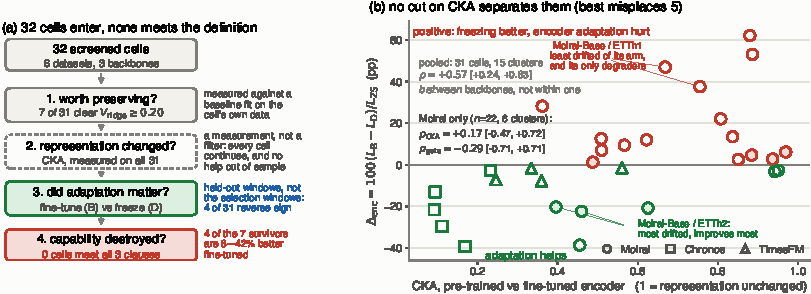
\includegraphics[width=\linewidth]{fig1_diagnostic_flow.pdf}
\caption{\textbf{(a)}~The screen of \S\ref{sec:method} over the 31 cells that
carry a selection-split gate: CKA filters none of them, and no cell meets the
degradation definition.  \textbf{(b)}~The same cells as CKA against held-out
$\denc$ (positive ${=}$ freezing better): no cut on CKA separates the cells
adaptation helped from the cells it hurt.  The labelled pairs are the running
example: Moirai-Base's two \emph{least} drifted cells are its only two that
degrade, and its two most drifted improve the most (\S\ref{sec:exp3}).  Filled
markers clear the gate; both $\rho$ are clustered by backbone${\times}$dataset,
and only Moirai has enough cells to estimate one within a backbone
(Appendix~\ref{app:clustered}).}
\label{fig:screen}
\end{figure}

\textbf{What we test, and on what.}  We screen \textbf{32 cells}: three backbones
(Moirai Small 13.8M, Base 91M, Large 311M; Chronos-T5~\citep{ansari2024chronos};
TimesFM-2.5~\citep{das2024timeseries}, with MOMENT~\citep{goswami2024moment}
screened and excluded), six datasets and two forecast horizons.  Each cell pairs
a full fine-tune with a frozen-encoder run, and on the Moirai cells with a strict
freeze under which nothing upstream of the forecasting head can move, at 3--10
seeds.  We then ask four questions in order (Figure~\ref{fig:screen}a).  Is
there a pre-trained capability worth preserving (\S\ref{sec:forecasting})?  Does
letting the encoder adapt help or hurt (\S\ref{sec:exp2})?  Does CKA order the
answer (\S\ref{sec:exp3})?  And where damage is forced, or looked for on other
datasets, does CKA see it (\S\ref{sec:exp4})?  Every claim is about the
checkpoints, datasets and protocols we evaluated; the readings we decline are
listed under \emph{Scope of the claims} in the Ethics Statement.

\textbf{Contributions.}
\begin{enumerate}\itemsep1pt
  \item \textbf{Drift does not track the intervention.}  Within Moirai-Base the
    least drifted cells are the only ones that degrade; a pre-registered positive
    control drives CKA on the original task's inputs to $0.063$ while that task
    \emph{improves} by $23.3\%$; and \pending{out-of-domain retention result}.
    Across cells, within Moirai, the only backbone with enough cells to ask,
    $\rho{=}{+}0.168$ (clustered CI $[-0.469,{+}0.717]$): an interval that rules out
    a strong positive association but not a moderate one, so we claim no ordering
    rather than the absence of one.  Out of sample, adding CKA to backbone and
    protocol lowers leave-one-cluster-out $R^2$ from $+0.201$ to $+0.176$
    (\S\ref{sec:exp3}).
  \item \textbf{Two measurement prerequisites for any such comparison.}  Scoring
    the frozen-encoder comparison on the windows it was selected on reverses its
    sign on 4 of 31 cells, all toward flattering the frozen encoder; and an unfitted
    linear baseline would move 17 of Moirai's 21 cells across the capability screen.
    With both in place, \textbf{only 7 of the 31 scored cells} show a pre-trained
    advantage over a linear regression fit on the target data, all of them Moirai
    on ETTh2 and ETTm2 (\S\S\ref{sec:method},~\ref{sec:forecasting}).
  \item \textbf{No harmful encoder adaptation under a prespecified definition.}
    On multiplicity-adjusted paired intervals the 31 cells split 2 freezing-better,
    4 adaptation-better and 25 inconclusive, and both freezing-better cells are
    ones the screen rejects; on five of the seven that pass it, full fine-tuning
    improves on zero-shot (\S\ref{sec:exp2}).
\end{enumerate}

% ============================================================
\section{Background and Related Work}
\label{sec:background}
% ============================================================

\textbf{Related work: three lines, and the gap between them.}
\emph{(i)~Forgetting} is studied in continual learning, NLP and fine-tuning
dynamics~\citep{kirkpatrick2017ewc, li2017lwf, luo2023forgetting,
kumar2022finetuning, andreassen2023evolution}, including sequential fine-tuning
of TSFMs~\citep{karaouli2025foundation}, and supplies the prescriptions
we test.  \textbf{This is not a continual-learning study}: no task sequence, no
loss on a prior task, one adaptation step, so ``forgetting'' here is degradation
relative to the same checkpoint's zero-shot on the same data, and a
catastrophic-forgetting result and ours can hold at once.
\emph{(ii)~TSFM adaptation} recipes span probabilistic
fine-tuning, generative pre-training, LLM reprogramming and cross-task
transfer~\citep{rasul2024lagllama, liu2024timer, jin2024timellm,
zhou2023onefitsall}, and are evaluated on target-task accuracy.
\emph{(iii)~Representation analysis} supplies the measurement (representation
similarity and probing~\citep{kornblith2019cka, hewitt2019structural,
pimentel2020information}), including work probing frozen TSFM internals
directly~\citep{wilinski2025representations}, where we instead track how
representations \emph{change under fine-tuning}.  CKA has been used to localise
forgetting~\citep{ramasesh2021anatomy}, and in vision classification a linear
probe shows that a large CKA drop can coexist with little loss of
knowledge~\citep{davari2022probing}; we ask the same question of TSFMs, against an
intervention rather than a probe.  \textbf{None of the three
establishes that the pre-trained representation was worth preserving on the
target task}, which is the premise (i)'s prescriptions rest on and what this
paper measures.

\textbf{Pre-training value gate.}
The gate is deliberately cheap and \emph{downstream-only}: the practitioner
runs the frozen model zero-shot on the target set and compares against a
lookback-96 linear regression \emph{fit on that same dataset}
(\S\ref{sec:method}), so neither pre-training data nor pre-training compute is
required.  We report $\Vb{b}$ as a continuous quantity for every cell
(Table~\ref{tab:r2task}) rather than only its verdict, and the $0.20$ operating
point is calibrated to ETT short-horizon benchmarks, where linear
baselines are famously competitive with deep
forecasters~\citep{zeng2023transformers}.  That competitiveness is the whole
reason the gate has teeth: \textbf{7 of the 31 scored cells clear it}, all on
Moirai and confined to two series, and in the other 24 the pre-trained model
has no measured advantage for fine-tuning to destroy.

\textbf{Task-level consequence: forgetting.}
We define forgetting as signed relative change in zero-shot-canonical
task metric on held-out test:
$\text{forg.\%} = 100 \cdot (M_{\text{FT}} - M_{\text{ZS}}) /
|M_{\text{ZS}}|$ (MSE for forecasting, so forg.${>}0$ means the fine-tuned model is
worse than the zero-shot one: \emph{task-level forgetting}).

\textbf{Decoupling harmful forgetting from benign specialisation.}
Representational change that redirects features toward the target
(\emph{benign specialisation}) must be separated from change that discards
generally useful structure (\emph{harmful forgetting}).  We separate them by
\emph{value-gate conditioning}:
change can be harmful only where the structure it discards was valuable, i.e.\ in
a gate-pass cell; in a gate-fail cell the same change is benign by construction,
because no demonstrated advantage existed to lose.  Gate-passing plus
forgetting${>}0$ is therefore necessary for harm but not sufficient, and whether
the encoder's \emph{change} carried the loss is settled by intervention (full
fine-tuning against a frozen encoder on the same data for the same epochs), and
not by observing the representation.

% ============================================================
\section{Protocol and Definitions}
\label{sec:method}
% ============================================================

\textbf{Models and training.}
Moirai~\citep{woo2024moirai} predicts a probabilistic distribution over the
horizon; we report MSE on the median of 20 forecast samples at $h{=}96$ and
$h{=}192$ (Appendix~\ref{app:moirai_median}).  Moirai is trained with AdamW
($\eta{=}10^{-4}$, weight decay $10^{-4}$), batch size 16 and gradient clipping
at 1.0, for 20 epochs with no early stopping: the 21 Moirai cells on ETT, Weather and
Electricity are read at their final epoch.  The other trainers select an epoch on
the selection windows (never the held-out ones): Moirai/ILI and TimesFM restore
their best epoch under patience 3 and 7, and Chronos keeps its best of 30 epochs
under full fine-tuning and trains its frozen-feature head to convergence
(Table~\ref{tab:trainers}).  \textbf{22 of the 31} cells train on $1{\text{k}}$
windows, and every table prints each cell's own $n$.  Reproducing a Moirai
fine-tune requires the \texttt{uni2ts} scaler patch of
Appendix~\ref{app:scaler_patch}.

\textbf{Three splits.}  The \emph{training} split fits the fine-tuning updates
and every baseline; the \emph{selection} split is where any checkpoint is chosen
and where the capability screen is scored; the \emph{held-out} split is disjoint
from both and is where every outcome is scored.  A cell's admission therefore
never uses the windows that later judge it.

\textbf{Capability screen.}  A checkpoint can only have a capability worth
preserving relative to something a practitioner could deploy instead, so the
baseline is part of the quantity: for a baseline $b$,
$\Vb{b} = 1-\text{MSE}_\text{ZS}/\text{MSE}_b$, positive when the zero-shot (ZS)
model beats $b$.  We threshold it at $0.20$, a prespecified operating point and
not an established boundary, and call the result the \emph{gate}.  Our primary
$b$ is one ridge map $\R^{96 \times F} \to \R^{h \times F}$ ($\lambda{=}10^{-4}$)
fit by least squares on the training windows and applied unchanged to the
selection windows.  It sees $96$ steps of context against the pre-trained
model's $96{+}h$, which if anything favours the pre-trained model;
\S\ref{sec:forecasting} also scores a ladder of eight baselines.

\textbf{Conditions.}  Full fine-tuning (B) updates every parameter.  The frozen
encoder (D) freezes the encoder stack but leaves the input projection and mask
encoding trainable, so its CKA is near but not exactly $1$ on Moirai
($0.889$--$0.9999$).  The strict freeze (H) also freezes those two modules,
so only the output head trains and the encoder's output is fixed by construction
(CKA exactly $1.000$).  LoRA ($r{=}8$), L2-SP and EWC are reported as a
mitigation spectrum in Appendix~\ref{app:full_tables}.
Figure~\ref{fig:freezeboundary} shows which modules move under each.

\textbf{The estimand.}  For a cell with $S$ paired seeds and a frozen arm F,
\begin{equation}
\label{eq:denc}
\denc \;=\; \frac{1}{S}\sum_{s=1}^{S} 100 \cdot
\frac{\mathcal{L}_\text{test}(\text{B}_s) - \mathcal{L}_\text{test}(\text{F}_s)}
     {\mathcal{L}_\text{test}(\text{ZS})},
\end{equation}
positive when freezing does better.  The shared zero-shot denominator only
rescales each cell so that different loss scales are comparable.  On Moirai, where
every cell has both controls, we lead with F${=}$H, the cleaner contrast, and
report F${=}$D beside it; across backbones we use F${=}$D, the one control all
three share.  The two disagree in sign on \pending{N of 22} Moirai cells
(\S\ref{sec:exp2}).  $\denc$ is the contrast the design \emph{manipulates}.
CKA is a \emph{post-treatment} measurement, taken on the object the treatment
changed, so it can only be a candidate predictor of $\denc$, and that is the
role we test.

\textbf{Representation diagnostics.}  Linear CKA~\citep{kornblith2019cka}
between pre-trained and fine-tuned representations, and weight drift ($\ell_2$
distance from the pre-trained parameters).  Every CKA in the body is of the final
encoder output, mean-pooled over tokens, on a fixed prefix of the selection split:
the comparison a practitioner holding two checkpoints can make without choosing a
layer or token position.  Token-flattened and per-layer variants and a
random-initialisation floor are in
Appendices~\ref{app:layerunfreeze} and~\ref{app:cka_calibration}.

\textbf{Definition (degradation of a demonstrated capability).}  A cell is a
degradation when (i)~$\Vb{b} \ge 0.20$ on selection windows, (ii)~full fine-tuning
ends worse than zero-shot, and (iii)~the frozen arm ends better than zero-shot,
which localises the loss to encoder updates rather than to the data or the epoch
budget.  Clauses (ii) and (iii) are tested as paired 95\% intervals on
$\text{B}{-}\text{ZS}$ and $\text{F}{-}\text{ZS}$, propagating the zero-shot
reference's error and adjusted across cells by Benjamini--Hochberg
(Appendix~\ref{app:pairedinference}), and also in the pre-registered form in
which every seed must agree.  \textbf{Both return the same count}.  Every ${\pm}$
in the body is a standard error over seeds.

\begin{center}
\fbox{\begin{minipage}{0.95\linewidth}
\small
\textbf{Two measurement choices that decide this result.}
\emph{(1)~Score the frozen-encoder comparison on windows you did not select on.}
Scoring $\denc$ on the selection windows instead reverses its sign on 4 of our 31
cells, and all four reverse toward flattering the frozen encoder
(\S\ref{sec:analysis:heldout}).
\emph{(2)~Fit the linear baseline.}  An unfitted per-window trend extrapolation,
a denominator a constant predictor beats, would move 17 of Moirai's 21 cells
across the threshold, 16 of them to gate-pass, and so reverse the conclusion
(Appendix~\ref{app:gatecorrection}).
\end{minipage}}
\end{center}

% ============================================================
\section{Experiment 1: Is There a Capability Worth Preserving?}
\label{sec:forecasting}
\label{sec:forecasting:gate}
% ============================================================

A claim that fine-tuning damages valuable pre-trained features needs a cell where
such features are demonstrably present.  Across \textbf{32 screened
cells} (21 Moirai: three capacities, five datasets, two horizons; 5
Chronos-T5, 5 TimesFM-2.5 and 1 Moirai/ILI), seven clear the gate, and all seven
are Moirai: five on ETTh2 and two on ETTm2.  The gate is scored on selection
windows, which exist for 31 of the 32 (TimesFM/Electricity has no paired
frozen-encoder run, so it is screened but carries neither a gate nor an
intervention row), and every denominator below is 31.

\textbf{Moirai: 7 of 21} (Table~\ref{tab:r2task}).  ETTh2 clears at every
capacity: Small $h{=}96$ ($+0.874$) and $h{=}192$ ($+0.932$), Base $h{=}96$
($+0.777$) and $h{=}192$ ($+0.925$), Large $h{=}96$ ($+0.875$).  ETTm2 clears
at two of four, Small $h{=}192$ ($+0.352$) and Base $h{=}192$ ($+0.211$).
Every other dataset fails at every capacity, and every failing cell is below the
baseline rather than short of the threshold.  Capacity does not help: Moirai-Base
is 6.6$\times$ larger than Moirai-Small and further behind the baseline on both
ETTh1 and Weather.

\textbf{Chronos-T5-Small: 0 of 5; TimesFM-2.5: 0 of 4}
(Table~\ref{tab:crossbackbone}).  All nine fall in a narrow band about zero,
$-0.275$ to $+0.082$.  On ETTh2, where Moirai clears at every capacity, Chronos
is below the fitted baseline ($-0.184$ on selection, $-0.325$ on held-out), so
the advantage is not a property of the dataset alone.

\textbf{One rung of eight.}  Scored against a ladder of eight baselines on the
same windows, with the training mean as an admissibility floor, \textbf{no cell of
the 31 clears $0.20$} against the strongest admissible rung it faces, and none
does on two further window sets.  \textbf{20 of the 31 clear it against at
least one admissible rung (14 Moirai, 3 Chronos, 3 TimesFM)}, and that union is
the scope of every drift analysis below, so those analyses span all three
backbones.  ``Seven cells clear the gate'' always means seven clear the fitted
ridge rung; per-rung counts, a matched-lookback baseline and the four cells a
near-constant rung would admit are in Appendix~\ref{app:baselines}.

\textbf{Prospectively, the gate is a conditioning device, not a detector.}
\label{sec:analysis:prospective}%
Predictions for eight unrun cells were committed to git before any of them was
trained.  None of the eight degraded and the gate flagged all eight
(\textbf{TP~0, FP~8, FN~0}), a test at zero prevalence that shows the gate's
positive predictions were wrong here and says nothing about its sensitivity.  A
second registered batch, on 9 of its 10 cells, gives specificity $0.78$
(Appendices~\ref{app:prospective2},~\ref{app:prospective3}).  What the gate does
is decide where the harm question can be asked at all: a cell that fails it has
no demonstrated advantage to lose, and 24 of our 31 fail it.

% ============================================================
\section{Experiment 2: Does Encoder Adaptation Help or Harm?}
\label{sec:exp2}
% ============================================================

\subsection{What Fine-Tuning Does to the Seven Survivors}
\label{sec:forecasting:results}

The seven cells Experiment 1 admits are the whole evidence base for a claim about
damage to valuable features, and they do not support one
(Table~\ref{tab:gate_survivors}).

\textbf{On four of the seven, full fine-tuning improves the checkpoint in every
seed.}  On Moirai-Base at $h{=}96$ and $h{=}192$ and Moirai-Large at $h{=}96$, all
on ETTh2, forgetting is $-31.4\%$, $-36.3\%$ and $-42.4\%$ against zero-shot,
negative in 3/3 seeds each, at CKA $0.460$, $0.396$ and $0.626$, the largest
representational change among the seven.  Freezing the encoder captures only part
of that gain ($-9.1\%$, $-16.1\%$, $-21.6\%$), so most of the improvement comes
from encoder adaptation.  The fourth, Moirai-Base/ETTm2 at $h{=}192$, improves by
$8.4\%$, and the frozen encoder does slightly better there ($-9.7\%$).

\textbf{On the remaining three, the mean harm does not survive inspection.}
Moirai-Small/ETTh2 at $h{=}192$ reads forg.$_\text{B}{=}{+}1.99{\pm}3.32$ with 5 of
10 seeds positive, the closest the matrix comes to degradation.  At $h{=}96$ the
positive mean ($+9.71{\pm}10.58$, 4 of 10 seeds) comes from one seed that diverges
under the frozen encoder too, an optimisation failure rather than an encoder
effect; we keep it in every mean.  Moirai-Small/ETTm2 at $h{=}192$ improves on
average ($1.10\%$) with 3 of 5 seeds harmful.

\subsection{Where the Freezing Boundary Is Drawn}
\label{sec:exp2:strict}

The ordinary frozen encoder (D) leaves the input projection and mask encoding
trainable, so a ``freezing wins'' reading could come from those modules adapting
rather than from the encoder staying fixed.  We therefore ran the strict freeze
(H) on every Moirai cell (\pending{22} cells, 3--10 seeds;
Table~\ref{tab:strictfreeze}).  B${-}$H and B${-}$D agree in sign on
\pending{N} cells.  They disagree on \pending{the four Moirai/ETTm2 cells
and any of the six new ones}, and on every disagreeing cell the strict control
moves toward adaptation: on ETTm2, Moirai-Small $h{=}96$ goes from B${-}$D
$+7.3{\pm}2.9$ to B${-}$H $-6.8{\pm}2.0$ and Moirai-Base $h{=}96$ from $+7.0{\pm}2.4$
to $-9.2{\pm}3.1$, so the apparent freezing advantage on that dataset was carried
by the input projection.  The strict freeze therefore recovers no degradation case;
it removes the ones D appeared to suggest.  All Moirai counts below are reported
under both controls.

\subsection{Held-Out Scoring Is a Precondition}
\label{sec:analysis:heldout}

Scoring $\denc$ on the selection windows instead of the held-out ones
\textbf{reverses its sign in 4 of the 31 intervention cells}, all in the same
direction: on the selection windows the frozen encoder wins, on held-out windows
full fine-tuning does (Table~\ref{tab:heldout_decomp}).  Two of the four are
among the seven gate-passing cells (Moirai-Base and Moirai-Large on ETTh2, which
move from $+3.8$ and $+7.2$ to $-22.3$ and $-20.8$).  A frozen-versus-full comparison
scored on the windows a checkpoint was selected on is therefore not a weaker
version of the held-out one; it can give the opposite answer.

\subsection{No Degradation Instance Survives a Prespecified Definition}
\label{sec:analysis:degradation}

The three-clause definition of \S\ref{sec:method} returns \textbf{zero cells} of
the 31, under both the interval and the registered form and, on Moirai, under
both controls.  Clause~(i) removes 24 outright: they have no measured pre-trained
advantage, so a worse score after fine-tuning replaces nothing demonstrated.
Of the seven that remain, four fail clause~(ii) with every seed agreeing, and
the other three fail it cell by cell (\S\ref{sec:forecasting:results}).
Relaxing the definition does not manufacture a case: across 8 rungs, at either
gate threshold, \textbf{the largest count anywhere is 2}, reached only when the
means clause is dropped altogether (Appendix~\ref{app:defsensitivity}).

\textbf{Per-cell inference.}  Paired $95\%$ intervals on $\denc$ (F${=}$D),
Benjamini--Hochberg adjusted across the 31 cells, call \textbf{2 cells
freezing-better, 4 adaptation-better and 25 inconclusive}; under F${=}$H on
Moirai, \pending{counts}.  The two freezing-better cells are Moirai-Small/ETTh1 at
both horizons, which the screen rejects, while two of the four adaptation-better
cells pass it, at $+0.925$ and $+0.875$.  A pre-registered seed top-up adds a third
freezing-better cell, which the screen admits (Moirai-Small/ETTm2 $h{=}192$,
gate $+0.352$), and the definition still returns zero
(Appendix~\ref{app:pairedinference}).  Most calls are inconclusive because the
design is underpowered for small effects, and we say so rather than read them as
null: the survivors' dispersion gives minimum detectable effects of
$4.7$--$14.7$~pp, and two survivors would need 182 and 212 paired seeds to
resolve their observed effect.  Over the 20 value-cells, $\denc{=}{+}0.7$ with
clustered CI $[-11.1,{+}14.1]$.  Changing the gate's estimator does admit cells
(persistence admits three and GBM one), but all four rest on a denominator within
$5\%$ of the training-mean floor, so a weaker baseline is what manufactures them
(Appendix~\ref{app:baselines}).

We do not conclude that fine-tuning never damages a pre-trained capability, only
that on these benchmarks we could not find one instance that meets its own
definition: no cell's advantage survives every admissible rung of the ladder, and
where the fitted-ridge advantage exists, fine-tuning on 500--1{,}000 samples
usually improves on it.

% ============================================================
\section{Experiment 3: Can Measured Drift Replace the Frozen Control?}
\label{sec:exp3}
% ============================================================

% 2026-09-25. Two sentences cut from this lead -- "CKA tells us that the representation changed;
% Experiment 2's intervention tells us whether the change was valuable" -- to pay for the seed-top-up
% scoping in the abstract and \S5.3. They restate, three lines early, the boldface claim this same
% paragraph ends on, and the abstract and the conclusion both carry the pair verbatim. The restatement
% went; the claim did not.
% Round 9. "This is the section the paper's title makes its claim in" became false when the title
% stopped asserting anything (see the round-9 block in main.tex). The replacement says the same thing
% about the PAPER rather than about the title, so it survives the next retitle: this section is where
% the empirical claim is argued either way, and the sentence is the same length, which matters on a
% body with no page slack.
This is the section the paper's empirical claim is argued in.  Neither CKA nor weight drift is manipulated by that design
(\S\ref{sec:method}), so both enter here only as candidate \emph{predictors} of
$\denc$, and \textbf{across the cells we evaluate, the former is not an
actionable substitute for the latter.}

\label{sec:forecasting:nonmoirai}
\textbf{Drift and outcome come apart inside a single backbone}: within our
Moirai matrix, the strongest form of the finding.  Beyond the sweep of
\S\ref{sec:forecasting:replication}: within Moirai-Base the two \emph{least}
drifted cells are the only two that degrade (ETTh1 at CKA $0.755$ and $0.669$,
$+22.8\%$ and $+39.5\%$) while its two most drifted improve the most within the
arm (ETTh2 at CKA $0.460$ and $0.396$, $-31.4\%$ and $-36.3\%$; the whole
eight-cell ordering is Appendix Table~\ref{tab:dissociation}); and inside
Moirai-Large's LoRA arm the learning rate, not the rank, decides the sign at
near-identical CKA ($0.973$ against $0.989$; Appendix~\ref{app:lora_rank}).
% 2026-09-26. Compressed, not cut: "we read the ordering as illustrative, claim no reverse relationship
% from $n{=}8$, and leave the negative result to the pre-registered test below" -> the first two clauses
% are what "a counterexample and nothing more" already says, and the third is the next paragraph's
% opening sentence. No chk() matched any of it ("illustrative", "n{=}8" and "no reverse relationship"
% are absent from check_paper_numbers.py), and the caveat survives in the words that carry it.
Eight cells are a \emph{counterexample} to ``low CKA means damage'' and nothing
more, with no reverse relationship claimed from $n{=}8$.

% 2026-09-26 (B5). Cut for the lines \S6's decision-pricing sentence needs: "whose $84.5\%$ advantage
% traces to no run record and does not reproduce". That is audit prose about a superseded figure, and a
% reviewer asked for less of it in the main text; app:m4 keeps the whole record -- it reproduces the
% superseded figure under the legacy estimator, prints the training mean that beats it, and names the
% three estimators -- and check_paper_numbers.py:3897-3918 registers every number of that reproduction
% with its sites there. The provenance claim itself was deliberately unchecked because there is no
% record to check it against, which is what made it the safest printed line in the body to give up.
% $+0.092$ STAYS: the "M4: the corrected gate, in the body" check has its only site in this sentence,
% and cutting the clause it matches failed the checker before this build -- which is what that check is
% for. The corrected gate is also the number this paragraph needs, since it is what makes the eleventh
% cell a gate failure rather than an exception.
\textbf{Near-identical drift, opposite consequences.}  Against the fitted baseline
none of the ten non-Moirai cells gate-passes, nor does the eleventh we re-ran to
check: Chronos on M4-Monthly, which scores $+0.092$ once the gate is computed as
defined (Appendix~\ref{app:chronos_detail}).  So what the two extra backbones supply
is architectural diversity and the dissociation itself, \textbf{not a controlled
% 2026-09-26. The horizon-and-normalisation half of this clause was a VERBATIM duplicate of Limitations
% item (4) ("the non-Moirai arm runs at h=24 and the Moirai arm at h in {96,192}, on different
% normalisations; we report them separately and never pool them"), which is the concession's own site and
% stays untouched -- a reviewer is scoring generalisation, so the concession is the copy to keep.
% ONE REGISTERED SITE MOVES: "the horizons, in the form the cross-backbone caveat uses"
% (check_paper_numbers.py:2597) goes from 5 sites to 4, which is above its floor of 1 and was verified by
% diffing per-claim site counts against HEAD rather than by reading the pass/fail line. What survives
% here is the operative half, that we never pool them, plus the pointer; \S\ref{sec:limitations} says why.
replication}: we read them qualitatively and never pool them
(\S\ref{sec:limitations}).  Four
of the five Chronos-T5-Small cells restructure to a degree that would, on the usual
reading, be called catastrophic (CKA ${\in}[0.092, 0.169]$, at or below the
$0.215{\pm}0.054$ an \emph{untrained} encoder of this architecture scores;
Appendix~\ref{app:cka_calibration}), yet outcomes across the five span
\textbf{$-41.4\%$ on ETTm2 to $+20.6\%$ on ETTh1}, a 62-point spread in which ETTh1
is the \emph{least} drifted and the only one that degrades; the four TimesFM-2.5
cells sit at milder drift and all improve
(Appendix Table~\ref{tab:crossbackbone}).
% Round 8 (B3). "But that pooled figure is a backbone artefact by our own rule" asserted the rule without
% stating it, and a reviewer read the within-backbone null as Simpson's-paradox special pleading -- the
% pooled +0.567 is not a small correlation, and a paper that reports it and then sets it aside owes the
% reason. The reason is that CONDITIONING is the whole point: backbone and protocol are known to the
% reader before any CKA is computed, so an association that lives between backbones cannot help them, and
% Figure 1b now prints the pooled rho beside the within-Moirai one with exactly that label. Both numbers
% were already here; what is new is the sentence saying which question each answers.
%
% "MEASURED THAT WAY," IS LOAD-BEARING PUNCTUATION, NOT A FLOURISH. This rewrite first made "within
% Moirai" the start of a sentence, which capitalised the W and silently dropped one of the six prose
% sites of check_paper_numbers.py's min_sites=5 "within-Moirai CKA rho" check -- 425 sites became 424
% with every claim still reporting ok, because the check still had five. The introductory clause exists
% to keep the phrase mid-sentence and lower-case. Any rewrite here has to leave "within Moirai, the only
% arm with enough cells to ask, $\rho{=}{+}0.168$" intact and uncapitalised: the pattern is
% case-sensitive and allows at most 70 characters between the phrase and the value.
Pooled across all 31 cells CKA does correlate with the intervention
($\rho{=}{+}0.567$, clustered CI $[{+}0.239,{+}0.828]$), which is not a small number
and not one a practitioner can use: backbone and protocol are known before any CKA is
computed, so the diagnostic has to order the outcome \emph{given} them rather than
pool three backbones and report the gap between two of them (Figure~\ref{fig:screen}b).
% Round 10 (A1/B3/C4). Three changes, and the first two are length-neutral by construction because the
% two positional patterns the comment above records still have to match: the clause
% "within Moirai, the only arm with enough cells to ask, $\rho{=}{+}0.168$" is untouched and
% "clustered CI" still follows the value within 25 characters.
% B3: the concession was a DEPENDENT clause -- "which admits a moderate positive relationship BUT does
% not provide a reliable ordering" -- and a reviewer's Priority 2 is that our statistical uncertainty
% should not be subordinated to our negative. It is now one of two things the interval does, in a
% coordinate structure, so a reader skimming cannot take the admission as a concession made in passing.
% Nothing is added or withdrawn: same interval, same claim, same length.
% A1: "reliable ordering" -> "reliable, actionable ordering", the third and last CKA site (see main.tex).
% C4: the decision price, one sentence, funded by the retrospective-variant cut in 03_protocol.tex. It
% leads with the row that cuts against us -- the prescribed orientation LOSES 6.97 pp -- and states in
% the same breath that the orientation which pays out of sample is the inverse of it, which is the part
% that is not a null result. The favourable-looking row (+7.47 pp, interval covering zero) is in
% app:decision under its own bold sentence rather than here, because one printed line cannot carry a
% point estimate, its interval and its post-hoc status without misleading on one of the three. The
% interval is in WHOLE percentage points: cka_decision_value.py --seedcheck shows two-decimal bounds do
% not reproduce across bootstrap seeds.
Measured that way, within Moirai, the only arm with enough
cells to ask, $\rho{=}{+}0.168$ with clustered CI $[-0.469,{+}0.717]$: an interval
that admits a moderate positive relationship, and that \textbf{does not provide a
reliable, actionable ordering} of our cells.  Priced as a decision, freezing where
drift is largest, as prescribed, is worth $-6.97$~pp $[-10, +14]$ against always
adapting; the orientation that pays out of sample is the inverse
(Appendix~\ref{app:decision}).  Nor does the
second diagnostic \S\ref{sec:method} defines rescue it: pooled $\ell_2$ weight
drift gives $\rho{=}{+}0.118$ with a CI including zero, and nor do five further
geometric measures
(Appendices~\ref{app:crosscell},~\ref{app:driftmetrics}).  The same dissociation
holds \emph{inside} one encoder: the two unfreeze depths we ran at 10 seeds each
(the top 3 of 6 layers, and all 6) are indistinguishable on the task at CKA
$0.716$ against $0.465$ (Appendix~\ref{app:layerunfreeze}).
% 2026-09-25. Cut: "And where a cell does degrade, freezing does not save it: on Chronos/ETTh1 the
% frozen encoder is worse still (+59.8% against +20.6%), so encoder adaptation is not the locus of the
% damage." It is cut for CORRECTNESS first and page-10 funding second. "Where a cell does degrade" is a
% statement about forg_B, and Chronos's per-condition forgetting is exactly the quantity this paper
% flags forg_confounded and excludes from every forgetting comparison it makes (cell_matrix.py:474,
% paired_inference.py:376, degradation_sensitivity.py:119): an MSE head is attached for B and D while
% the zero-shot reference is the native decoder's. The B-vs-D CONTRAST survives that confound (the
% mismatched denominator rescales it and cannot flip its sign), but the premise this sentence builds on
% does not, and the Ethics Statement's Scope paragraph now says out loud that these five cells are
% excluded wherever a forgetting comparison is made -- which this sentence was. Both numbers stay in
% tab:crossbackbone, where crossbackbone.tex is emitter-written and the row carries its confound mark,
% so the reader still has them with the caveat attached; what is gone is the body's inference from them.

% 2026-09-25. "A wide interval is a failure to establish an ordering, not evidence against one" cut
% here, same page budget. The caution is not dropped: this paragraph still closes on "a null in
% prediction rather than evidence of no relationship", and app:loco states it as its own sentence.
\textbf{We find no evidence that CKA improves prediction beyond backbone identity.}  With
the ladder and deciding statistic fixed in advance
(\texttt{results/preregister\_loco.json}) we asked out of sample whether measuring
CKA helps a reader who already knows the backbone, the horizon and $n$.  It does
not: leave-one-cluster-out $R^2$ over the 15 clusters rises from $+0.000$ to
$+0.137$ on backbone identity and $+0.201$ with horizon and $\log n$, then
\emph{falls} to $+0.176$ once CKA is added ($\Delta R^2{=}{-}0.025$; no help in
$69\%$ of cluster-bootstrap draws), and the backbone-specific-slope variant is
worst of all at $+0.019$.  So the predictable part of $\denc$ is predictable from
protocol identity, though the slope itself, $+43$~pp per unit CKA with a cluster
interval of $[-31, +107]$, makes this a null in \emph{prediction} rather than
evidence of no relationship (Appendix~\ref{app:loco}).

% Two paragraphs were cut from here on 20 Sep 2026: the graded-screen robustness check (rho on the 20
% gate-clearing cells against the 11 others, and the b_3 interaction) and the ILI case study's numbers.
% Both are reported in full in the appendices pointed at below, which is where they were already
% reported -- the body was restating them. Cut so that this section spends its lines on the
% dissociation itself, which is the paper's one sentence, rather than on two objections it also answers.
%
% The two one-sentence SUMMARIES that survived that cut moved on 21 Sep 2026, VERBATIM, to
% app:valueaxis and app:ili_gate respectively, to fund \S\ref{sec:exp4:poscontrol} on a 9-page body
% with no slack. Verbatim rather than reworded because each carries a claim registered in
% scripts/check_paper_numbers.py at min_sites=1 ("cells with nothing to lose"), so a reworded move
% would have silently dropped the paper's only site for it. \label{sec:analysis:ili} moved with its
% paragraph and the three \S\ref sites that pointed at it now point at Appendix app:ili_gate; the
% label is gone rather than left behind pointing at a section that no longer discusses ILI.


% ============================================================
\section{Experiment 4: Does CKA See Damage Where It Can Occur?}
\label{sec:exp4}
% ============================================================

Every cell above is fine-tuned and scored on the same series, so Experiments 2
and 3 measure what adaptation does to the target task.  Forgetting proper is a loss
of what the model could do elsewhere, and a diagnostic cannot be shown to miss
damage that never occurred.  This section looks for damage in the two places it
can occur: on a task constructed to conflict with the pre-trained prior, and on
datasets the model was not fine-tuned on.  Both arms were pre-registered, with
thresholds and outcomes committed before the first run.

\subsection{A Positive Control: Near-Orthogonal Drift, and the Capability Survives}
\label{sec:exp4:poscontrol}

Task A is the strongest capability the screen admits (Moirai-Small/ETTh2,
$h{=}192$, $\Vb{\text{ridge}}{=}{+}0.932$).  Task B is a synthetic series, fixed
by hash before any run, whose correct forecast is the \emph{negation} of the
seasonal-naive prior, task A's own strongest admissible baseline.  We fine-tuned
on B under $\text{lr}\in\{10^{-4},10^{-3},10^{-2}\}$ with both encoder conditions
at 3 seeds and measured A (Appendix~\ref{app:poscontrol}).  Task B was learned in
\textbf{21 of 21} runs (minimum $+56.6\%$ against a registered $20\%$).  At the top
rung CKA on task A's inputs falls to $0.063$ and $\ell_2$ drift reaches $2795$,
against $0.999$ and $7.2$ at the gentlest, and task A gets \emph{better}, by
$23.3{\pm}2.0\%$ in every seed; across the 21 runs CKA and retention correlate at
$\rho{=}{+}0.466$, the wrong sign for a damage detector.  The registered
destruction threshold (retention loss ${\geq}50\%$ in a majority of seeds) was
never reached: the worst run lost $26.7\%$.  A representation can be driven most
of the way to orthogonality by training in conflict with a capability, and the
capability survives.

\subsection{Out-of-Domain Retention}
\label{sec:exp4:ood}

We fine-tuned each of the seven gate-passing Moirai cells under full
fine-tuning, the frozen encoder and the strict freeze (3 seeds each) and scored
every final checkpoint zero-shot on the held-out windows of the four datasets it
was not trained on, measuring CKA on those datasets' own inputs
(Appendix~\ref{app:ood}).  The registered threshold for harmful forgetting is a
loss at least 10~pp larger under full fine-tuning than under the strict freeze, in
every seed.  \pending{Result: how many (cell, dataset) pairs meet it; retention
range for B, D, H; Spearman between 1$-$CKA and retention with its cell-clustered
interval; which registered outcome (O1/O2/O3) fired.}

% ============================================================
\section{Limitations}
\label{sec:limitations}
% ============================================================

(1)~\emph{One backbone carries the within-backbone evidence.}  The seven
gate-passing cells and the within-backbone association are Moirai on two
series; Chronos and TimesFM gate-fail everywhere and use different trainers, so
they show the dissociation but do not replicate the analysis
(\S\ref{sec:exp3}).  \pending{second-family runs on gate-passing datasets, if
completed}.
(2)~\emph{A null is not a proof of absence.}  What would settle the harm question
is a cell with a large pre-trained margin over a strong baseline, which these
benchmarks do not supply (\S\ref{sec:forecasting}).
(3)~\emph{Seed counts are small}, 3 to 10 per cell, so most per-cell calls are
inconclusive by construction (\S\ref{sec:analysis:degradation}).
(4)~\emph{Horizon differs by backbone}: $h{=}24$ for Chronos and TimesFM,
$h{\in}\{96,192\}$ for Moirai, so the two are never pooled.
(5)~\emph{Out-of-domain retention is measured on the paper's own benchmarks}, not
on Moirai's pre-training corpus (\S\ref{sec:exp4:ood}).
(6)~\emph{We measure whether restructuring was necessary, not what it changed}:
linear probes on these encoders do not generalise under a temporal split
(Appendix~\ref{sec:retraction}).  Further detail is in
Appendix~\ref{app:limitations}.

% ============================================================
\section{Conclusion}
\label{sec:conclusion}
% ============================================================

Representation drift is widely read as forgetting.  Against the intervention it
stands in for, on three time-series foundation models and six benchmarks, that
reading does not hold: the least drifted cells can be the ones that degrade, a
representation driven nearly orthogonal can retain its capability, and CKA adds
nothing to what backbone and protocol already predict.  On the target task we
could not find one cell where fine-tuning demonstrably damaged a pre-trained
capability; on datasets it was not tuned on we found eleven, and CKA did not order
them.  None of this makes CKA a poor
measure of similarity; it makes similarity a poor measure of harm.

The practical advice follows from the two measurement choices that decided our
results.  First check that the pre-trained model beats a baseline fitted on your
own data, because a forgetting result on a cell with no pre-trained advantage is a
statement about the benchmark.  Then compare full fine-tuning against a strictly
frozen encoder on windows neither run selected on.  That comparison costs one
extra training run, and it answers the question drift only appears to.


% Ethics and Reproducibility statements. ICLR excludes both from the 9-page
% main-text limit, so these must stay AFTER the conclusion -- the body ends
% flush with the bottom of page 9 and has no slack.
% ============================================================
% Ethics, Reproducibility and AI-assistant statements.  ICLR excludes these from the 9-page
% main-text limit, so nothing here competes with the body for space.  They are
% placed after the conclusion and before the references, per the ICLR template.
% ============================================================

\section*{Ethics Statement}

\textbf{Data.}  Every experiment uses public benchmark data and involves no human
subjects and no personally identifying information.  The forecasting datasets
(ETTh1, ETTh2, ETTm2, Weather and Electricity) are standard public
releases of instrument and utility measurements.  The ILI cell uses public
aggregate influenza-surveillance counts, not individual health records.  The IoT
negative control uses N-BaIoT, network traffic captured from a laboratory
testbed of consumer devices rather than from a deployed network.  We introduce no
new data collection.

\textbf{The main risk in this paper is that its negative result is read too
broadly.}  We report that on these benchmarks we could not construct a cell in
which fine-tuning demonstrably damages a pre-trained capability, and that a
diagnostic we proposed for predicting such damage has no positive instance to
predict.  That is a statement about six standard forecasting benchmarks and three
backbones, and \S\ref{sec:limitations} states what it does not license.  It is
\emph{not} evidence that fine-tuning is safe in general, and a practitioner who
reads it as permission to skip the frozen-encoder control would be drawing the
opposite of our recommendation: our prescription is to \emph{run} that control,
because we found the observational shortcuts unreliable.  Domains where a
pre-trained checkpoint holds a large, well-established advantage (which these
benchmarks do not, on 24 of the 31 cells we screened) are exactly where the
question remains open.

\textbf{Scope of the claims: one adaptation protocol, not fine-tuning in
general.}  Three facts bound every number in this paper, and we state them
together here rather than leaving them to be assembled from three appendices.
\emph{(i)~The training objective differs by backbone, and one of the three is not
native.}  Moirai is fine-tuned through its own probabilistic NLL, and TimesFM
through its own point head's loss (MSE on the mean channel plus pinball on the
nine decile channels), with no head attached to either.  The five
Chronos-T5-Small cells in the main matrix are instead fine-tuned through an
\emph{added} MSE regression head on mean-pooled encoder features, which bypasses
the tokenised cross-entropy Chronos was pre-trained with.  That mismatch is why
Chronos's per-condition forgetting is flagged confounded in the code and excluded
wherever a forgetting comparison is made (Appendix~\ref{app:predictor}), and why
the M4-Monthly arm, which \emph{is} fine-tuned through the native cross-entropy,
is reported separately (Appendix~\ref{app:chronos_detail}) instead of pooled with
those five.  \emph{(ii)~The outcome is one metric on one channel.}  Every
forecasting result is MSE on a single target channel at a fixed horizon; we test
no multivariate-target, multi-task or classification adaptation beyond the IoT
negative control.  \emph{(iii)~One adaptation step, not a task sequence}
(\S\ref{sec:background}).  ``Encoder adaptation'' in this paper therefore means
what this protocol does, and our results say nothing about a backbone fine-tuned
through its own decoder on a task we did not run.

% Round 8 (C1/C2), and it is HERE rather than in the body for one reason: ICLR excludes these statements
% from the 9-page limit, the body has zero slack, and a reader who wants the boundary of a negative result
% is a reader who will follow one pointer to find it. S1's scope paragraph points at this list by name.
%
% Every item below is a reading a reviewer of the previous draft actually offered back to us as our
% claim, so this is not a list of straw positions -- it is the set of five things the paper was read as
% saying and does not say. Two of them were named inline in S1 until this round ("we do not claim that
% fine-tuning is safe, nor that foundation models are useless for forecasting"); they are items (iii)
% and (v) here, so the enumeration replaces those two rather than adding to them.
\textbf{What we do not claim.}  Five readings of this paper's negative results are
ones we explicitly decline.  \emph{(i)}~That CKA fails to measure representation
change: it does measure it, and we use it as a measurement throughout --- what we
test is whether that measurement substitutes for an intervention.
\emph{(ii)}~That CKA can never predict downstream utility.  We report that it does
not reliably order the intervention outcome across the cells we ran, with the one
backbone family large enough to condition on carrying the cleanest evidence; a
larger matrix, another family or another protocol could show otherwise.
\emph{(iii)}~That fine-tuning never causes catastrophic forgetting, or that
fine-tuning is safe.  We could not construct a cell on these benchmarks in which it
demonstrably destroys a demonstrated capability, which is a failure to demonstrate
and not a demonstration of absence.  \emph{(iv)}~That freezing, L2-SP, EWC or
low-rank adaptation are useless.  Our prescription is to \emph{run} the
frozen-encoder control rather than to skip it, because it is the observational
shortcuts we found unreliable, not the mitigations.  \emph{(v)}~That foundation
models are useless for forecasting, or that these results establish the absence of
encoder-adaptation effects in time-series foundation models in general: seven of 31
cells cleared a deliberately weak screen, and the domains where a pre-trained
advantage is large and well established are exactly where the question stays open.
What we do claim is narrower than any of those: \textbf{within the intervention
cells we evaluated, and with the cleanest evidence inside the Moirai family, CKA
is not an actionable substitute for the intervention, and no cell meets our
prespecified criterion for harmful encoder adaptation.}
Appendix~\ref{app:claims} tabulates every claim we do make with its evidence and its
strength.
% The pointer to app:claims lives here because the conclusion's copy of it went with the disclaimer this
% list replaced (see the comment in 09_conclusion.tex). An appendix nothing in the paper points at is an
% appendix no reader reaches, so the reference had to land somewhere, and the paragraph enumerating what
% we do NOT claim is the right neighbour for the table of what we do.

\textbf{The value gate is a screen, not a verdict on a checkpoint.}  A cell that
fails the gate is one where the pre-trained model does not beat a linear regression
fit on that cell's own target data; it is \emph{not} a cell we claim holds no
pre-trained knowledge, and $\Vb{b}$ is a property of the (checkpoint, dataset,
baseline) triple rather than of the checkpoint (\S\ref{sec:method}).  The screen's
role is to decide where the question ``was something valuable destroyed?'' is even
askable.  Two things follow that are easy to misread.  Failing cells here fail
\emph{widely}: every failing Moirai cell is below its baseline rather than short of
the $0.20$ threshold, so the emptiness of the screen is not an artefact of where the
bar sits.  And gate-failing cells are still measured and still reported --- CKA,
$\denc$ and the paired intervals are computed on all 31 --- because the dissociation
between drift and outcome is a claim about the measurement, not about the survivors.

\textbf{Broader impact.}  This is a diagnostic study on public forecasting
benchmarks, and the effect we intend is to raise the bar for claims about
forgetting in time-series foundation models: a paper reporting that fine-tuning
damaged pre-trained features should say what baseline established that the
features were valuable, and how that baseline was fit.  Our own screen is the
worked example of why: the earlier version of this work reported eight
degradation cells on a baseline a constant predictor beats.  The controlled
comparison remains the way to answer the question for any particular cell, and
\S\ref{sec:analysis:degradation} claims only that the harm cannot be demonstrated
on these benchmarks.

\textbf{Research integrity.}  This version corrects an earlier version of the
same work in two ways that changed its conclusions rather than its presentation,
and we flag both rather than absorbing them silently.  An earlier version's value
gate used an unfitted per-window trend extrapolation as its linear baseline; a
constant predictor beats that baseline, and correcting it changes the gate status
of 17 of the 21 Moirai cells and removes every degradation instance the paper had;
that is, the entire class of cell the diagnostic was built to
predict.  Separately, we retract a linear-probe diagnostic
reported earlier: the statistic it rests on is non-zero only where the probe
fails to generalise, and Appendix~\ref{app:orthogonal} reports the measurement
that establishes this on the same encoders.  Neither correction required
re-running a model; both are documented with their audit trails in
Appendix~\ref{sec:retraction} and Appendix~\ref{app:gatecorrection}.  Where a
number in an earlier version could not be traced to a run record, we say so at
the site rather than reprinting it.

\textbf{Compute.}  The experiments are small by contemporary standards: no run
exceeds 10{,}000 training windows, and the sweep reported here runs on a single
GPU or on Apple silicon.  We report the protocol deviations forced by the
hardware available (Appendix~\ref{app:layerunfreeze}) rather than presenting the
runs as environment-independent.

\section*{Reproducibility Statement}

The paper is organised so that every quantity can be traced to a stored run
record, and we have tried to make the failure modes we hit ourselves cheap for
others to avoid.

\textbf{Where the numbers come from.}  Every table the source
\texttt{\textbackslash input}s is written by a named emitter that reads the per-run
JSON records (none is assembled by hand), and
\texttt{scripts/rederive\_all.sh} runs all of them in one command and then reports
which generated files changed.  A clean run means the PDF agrees with the run
records; any diff is a number that was stale.  There is one exception and it is
marked where it appears: the two inline tabulars in \S\ref{sec:retraction}
transcribe a \emph{withdrawn} computation whose probe records are too sparse to
re-derive, and they support no claim in this paper.  The per-run records carry the
fields the tables use (\texttt{final\_cka}, \texttt{forgetting\_pct},
\texttt{final\_val\_mse}, \texttt{final\_weight\_drift} and the early-stopping
block), together with the seed, epoch budget and sample count, so the dispersion
conventions can be recomputed rather than taken on trust.

\textbf{What ``reproducible'' means here, exactly, and what it does not.}
Auditability is not independent reproduction, and we distinguish three tiers
rather than letting the stronger word cover the weaker work.  \emph{(i)}~Every
table and figure is re-derivable from a clean clone with no data and no
checkpoints, because the run records are in the release; that is what
\texttt{rederive\_all.sh} checks.  \emph{(ii)}~Re-running the value gate or any
fine-tuning cell additionally needs the benchmark CSVs, which are public but not
ours to redistribute.  The obstacle there is not the download but knowing you
fetched the same file: ETT and Weather circulate in variants that differ in column
order and date parsing, and a variant with the same name changes every window and
so every MSE.  \texttt{results/data\_manifest.json} therefore records the
SHA-256, shape and date range of each CSV we used, and
\texttt{scripts/data\_manifest.py --check} verifies a local copy against it.
\emph{(iii)}~The drift-metric battery's geometry pass needs the fine-tuned
encoders themselves, which are excluded for size; its stored output is released,
so the table is re-derivable even though the measurement behind it is not.
\textbf{No third party has run any of this.}  What we offer is re-derivation from
committed run records and a bounded two-cell from-scratch check, not independent
replication.

\textbf{What the two-cell check found, and why we report it rather than a
tolerance.}  \texttt{scripts/rerun\_two\_cells.sh} retrains one Moirai cell
(Small/ETTh2 $h{=}96$, $n{=}500$, seed 42, full fine-tuning~(B)) and one non-Moirai
cell (TimesFM/ETTh1 $h{=}24$, $n{=}1{,}000$, seed 42, the same condition) from the raw
CSVs
and diffs every stored field.  \textbf{TimesFM reproduces exactly}: all nine
fields, including CKA and weight drift, are bit-identical.  \textbf{Moirai
reproduces its MSEs to within a few percent but not its forgetting percentage}:
zero-shot MSE moves $-0.8\%$, held-out MSE $+0.8\%$, the selection-window MSE
$+3.2\%$, CKA $-0.6\%$ ($0.957$ to $0.952$), and weight drift $+25.2\%$, while
forg.$_\text{B}$ moves from $+6.81$ to $+11.14$, a $63.5\%$ relative change.
That last figure is the informative one and it is not a failure of the smaller
ones, it is those smaller ones compounded: forg.$_\text{B}$ is
$(\text{MSE}_\text{val}-\text{MSE}_\text{ZS})/\text{MSE}_\text{ZS}$ on two nearly
equal quantities, so a $-0.8\%$ move in the denominator against a $+3.2\%$ move in
the numerator's larger term is amplified into $+63.5\%$ in the ratio.
% 2026-09-26 (B5). A reviewer asks the paper to de-emphasise percent-of-zero-shot metrics, citing this
% very reproduction as evidence that they are unstable. They are right about the metric and the
% instability was already reported here -- but as ARITHMETIC ABOUT ONE CELL. `grep -rn "amplif"` over
% every .tex in paper_8 returned exactly one line, the one above, so the paper had the instance and never
% the general statement, which is the weaker of the two things to have.
% Two sentences, and the SECOND is the one that matters, because it is the bound: the amplification is a
% property of forg_B, and \denc does not inherit it. That was already derivable from 03_protocol.tex:96-99
% ("Both arms share the zero-shot denominator, so $\denc$ is the raw contrast ... rescaled per cell") but
% nothing anywhere connected the two, so a reviewer reading S9's 63.5% had no way to see that the paper's
% headline quantity is not exposed to it. THE CLAIM IS DELIBERATELY LIMITED TO THE SIGN: a per-cell
% rescaling by a shared positive quantity cannot flip the contrast, but it can reorder cells against each
% other, so "sign" is what is claimed and not "ordering".
% This whole statement sits after \section*{Conclusion} and is excluded from the 9-page limit
% (main.tex:202-205), so it costs the body nothing -- which is why the generalisation goes here and not
% in \S5.
This is a property of the percent-of-zero-shot scale rather than a fact about this
cell: wherever the fine-tuned and zero-shot losses are close, a ratio of their
difference to one of them magnifies absolute moves that are themselves small, which
makes forg.$_\text{B}$ the least stable quantity this paper reports.
\textbf{$\denc$ does not inherit that instability}: both arms share the same
zero-shot denominator, so $\denc$ is the B-versus-D contrast rescaled per cell
(Equation~\ref{eq:denc}), and a shared positive rescaling cannot change its sign,
which is what every claim in the paper is stated in terms of.
Moirai scores the median of 20 sampled forecasts and TimesFM emits a point
forecast, which is why only one of the two is reproducible to the bit.  Every
sign-bearing field kept its sign, which is what the paper's claims are stated in
terms of, but a reader should treat any single-seed Moirai forgetting figure as
carrying at least this much run-to-run variation, and that is why the paper
reports cells at 3--10 seeds with a dispersion and never a single run.

\textbf{Two things are required to reproduce the Moirai runs at all.}  First, the
\texttt{uni2ts} \texttt{PackedStdScaler} performs an in-place write that silently
detaches the gradient tape for losses depending on scaled statistics; without the
patch of Appendix~\ref{app:scaler_patch} training can appear to run while not
converging.  Second, the frozen-encoder condition is not a strict freeze (the
input projections and mask encoding remain trainable, which is why its CKA is not
$1.000$), and the strictly-frozen variant is reported separately
(Appendix~\ref{app:strictfreeze}).  Comparisons against a ``frozen'' baseline are
not comparable across papers unless which parameters were frozen is stated.

\textbf{Scoring protocol.}  All headline comparisons are scored on windows
disjoint from the ones used for selection.  This is not a refinement:
\S\ref{sec:analysis:heldout} shows that scoring on the selection windows instead
reverses the sign of the frozen-encoder comparison in 4 of the 31 intervention
cells, always in the same direction.  Reproducing our numbers therefore requires
reproducing the split discipline, and Appendix
Table~\ref{tab:heldout_decomp} gives the per-arm decomposition needed to check
which split a given number was scored on.

\textbf{Pre-registration.}  The prospective test of
\S\ref{sec:analysis:prospective} was registered before any outcome run for
those cells existed: \texttt{results/v47\_prospective/preregistration.json} for
the first batch and \texttt{results/v57\_prospective3/preregistration\_v3.json}
for the second, each committed before the first condition-B or condition-D run
of its own arm was launched.  The scorer,
\texttt{score\_prospective.py}, reads those files and the finished runs and makes
no decisions of its own.  All are in the release, and each registration's commit
precedes every run it scores.  \textbf{That ordering is checkable in the
version-control history, and the supplementary archive does not carry one.}  What
travels with the archive is each registration's own \texttt{written\_utc} and the
commit hash it was written at; the per-run records store no timestamp, so the
archive alone cannot order them against it.  We state the limit rather than let
``checkable'' cover a check the archive does not support: from the archive a
reader has the hashes and our word, and the ordering itself is verifiable against
the repository released with the paper.  The Chronos/M4-Monthly re-run of
Appendix~\ref{app:chronos_detail} carries a second registration
(\texttt{results/chronos\_m4/preregistration.json}), on the same terms and with
the same check available.  That arm is \emph{not} prospective (the superseded
runs' outcome was already known), so what its registration fixes is only what
was still fixable: the gate's estimator and split, the seeds, the decision rule,
and what each gate outcome would be taken to mean.  The gate was computed after
that file was committed, which matters because the estimator was itself one of
the things being corrected.
% The ladder top-up's registration, named here on the same footing as the other two non-prospective
% ones. This section is page-exempt, so there is nothing to trade against naming it, and the appendix
% that reports the rungs cites the same file. What makes it worth a sentence is the last clause: the
% outcome that fired is the one the registration called inconvenient in advance, so the rule that
% decided what the body says was fixed before the runs rather than chosen after them.
The $N{=}4$ and $N{=}5$ rungs of Appendix~\ref{app:layerunfreeze} carry a third
(\texttt{results/v49\_layerunfreeze\_10seed/preregistration\_ladder.json}),
committed before the first of their six runs.  It is also not prospective, and
what it fixes is the rungs, the seeds, the condition and flag, the reported
statistic, and \textbf{what each outcome would mean for the body}: that a
non-monotone forgetting profile across depth, or a thin rung landing outside the
matched pair's range, would be reported as found with the body's claim narrowed to
the matched pair rather than the ladder being dropped.  Both of those outcomes
occurred, and that is the rule we followed.

\textbf{The figures check themselves.}  Both generated figures read their values
from \texttt{scripts/cell\_matrix.py} and \emph{assert} at draw time every count the
body quotes from them: the number of gate-passing cells, the number of degradation
cells, the number of sign reversals and the sign of each correlation.  A run record
that moved would fail the figure rather than change it silently, which is the one
staleness path the table emitters do not cover.  (This sentence used to sit in the
caption of Figure~\ref{fig:screen}; it is a statement about the release, and the body
has no page to spare for it.)

\textbf{What we release.}  The analysis and experiment scripts, the per-run JSON
records behind every table, the emitter for every table and the one-command
re-derivation script, the benchmark-data manifest, every pre-registration file, and
the \LaTeX{} source and style files needed to build this paper.  Model checkpoints
are excluded for size; the appendices state which runs retained a checkpoint,
because two re-measurements we would otherwise have made were blocked by runs
whose checkpoints were not kept (Appendix~\ref{app:noisefloor}).

% ============================================================
% Required by the ICLR 2027 main track.  Placed with the other statements, after the
% conclusion and before the references, on the same footing as Ethics and
% Reproducibility.  Written to be checkable rather than reassuring: the commit count
% below is a fact about the released history, and the division between what the
% assistant produced and what it could not produce is the same division the
% Reproducibility Statement already enforces mechanically.
% ============================================================
\section*{Use of AI Assistants}

An LLM-based coding assistant (Anthropic's Claude, used through Claude Code) was
used in this work: \textbf{the majority of commits in this project's
version-control history carry an AI co-author trailer}.

\textbf{Where it was used.}  Implementation and prose. It wrote the initial draft of most
of the analysis and experiment scripts, including the table emitters, the
one-command re-derivation sweep, the prose-number checker, the figure scripts, and
the anonymity and bundle-inventory gates; and it drafted and edited some of the sections of the paper's
text.

\textbf{Where it was not used.}  It produced no experimental result.  Every number
in this paper comes from a run that executed and wrote a JSON record, and the
registered checks in \texttt{scripts/check\_paper\_numbers.py} compare the prose
against those records, never against anything a model asserted.  The
research question, the study design, the pre-registered predictions and decision
rules, the choice of what to cut and what to report, and every claim the paper
makes are ours.

% The venue's AI policy asks for an explicit affirmation that the AI-assisted work was reviewed, and
% the boilerplate it ships states it in these words. Added verbatim rather than left implicit in
% "full responsibility": the policy makes an undisclosed or unaffirmed use a Code of Ethics matter,
% and this section is exempt from the page limit, so there is nothing to trade against saying it.
\textbf{Responsibility, and one caveat.}  We have reviewed all AI-assisted work
in this paper, and we take full
responsibility for everything in it, errors introduced during
AI-assisted work included.  Such errors did occur, and the two kinds we hit
repeatedly are worth naming:
tables whose numbers had been typed by hand and then drifted from the records
they were supposed to summarise, and claims that were reworded in one place while
a restatement elsewhere kept the superseded figure.  Neither was caught by
rereading the paper; each was caught by a mechanical check.  That is the reason
the verification apparatus described above exists in the form it does, and it is
the part of this methodology we would recommend to anyone writing a paper this
way.


% ============================================================
\bibliographystyle{iclr2027_conference}
\bibliography{bibliography}
% The retraction used to be its own \input here. It is now the last subsection of
% "Audit trail and withdrawn analyses" at the end of sections/appendix.tex, together with
% the corrections summary, the gate-baseline correction and the ILI withdrawal: one place
% for every withdrawn reading, so a reader auditing the record reads one section.
% The labels sec:retraction, app:corrections, app:gatecorrection and app:ili_gate all survive.
% ============================================================
% Consolidated Appendix
% ============================================================
\newpage
\appendix
% A1, A2, ... rather than the class default \Alph{section}: the appendix now has more than 26
% sections, and \Alph overflows with "Counter too large" at the 27th. A1-style numbering also reads
% unambiguously next to the body's numbered sections, which single letters did not.
\renewcommand{\thesection}{A\arabic{section}}

% \appendix switches the numbering but prints no title, so the notation note below used to open
% page 14 as a bare italic paragraph directly under the running head, with the references ending
% on the page before and the first heading (A1) only after it. It read as orphaned text rather
% than as the front matter of the appendix. A starred heading gives it something to sit under and
% does not touch the A1..A29 numbering, since \section* leaves the counter alone.
\section*{Appendix}

\noindent\emph{Notation.} The appendices write the paper's estimand in its
condition form, $\text{B}{-}\text{D}$, because they compare conditions directly
(for instance $\text{B}{-}\text{D}$ against $\text{B}{-}\text{H}$).  It is the
same quantity the body calls $\denc$; the two are interchangeable throughout.

% ============================================================
\section{What This Paper Claims, and What It Does Not}
\label{app:claims}
% ============================================================
% Added 21 Sep 2026. The distinction between these three claims has been in the conclusion's last
% paragraph since round five, and a reviewer still read the paper as asserting the broad version. That
% is a fair reading of where we put it: a scope restriction stated once, in one sentence, at the end of
% nine pages, after a title that invites the broad version, is a restriction most readers will not
% reach. So it is a table now, in one place, with each claim's evidence and strength beside it -- and
% the three readings we do NOT make are rows of the same table rather than a trailing disclaimer,
% because they are the three a reader is most likely to supply unprompted.
%
% ON THE NUMBERS. Every figure in this table is written in the SAME words as a site the body already
% carries, so the patterns in scripts/check_paper_numbers.py that pin the body pin this table too. That
% is deliberate and it is the opposite of the usual instinct to reword for variety: a restatement in
% fresh words is a site no check reaches, and this project has already had ten tables drift that way.

Three claims of unequal strength are made in this paper, and they are not
interchangeable.  \textbf{C1} is a null in \emph{prediction}, established out of
sample under an analysis registered before it was run.  \textbf{C2} is a positive
claim about what the screen does, at an operating point we chose rather than
derived.  \textbf{C3} is methodological, and it is the only one of the three we
would defend outside these benchmarks.

\begin{table}[ht]
\centering\small
\caption{The paper's three claims with their evidence and their strength, and then
the three readings we do \emph{not} claim.  The rows are ordered by how far each
travels: C1 holds for the cells we evaluate, C2 for the screen at the threshold we
state, C3 for any study that reads a post-treatment similarity statistic as
evidence about a treatment's value.  The three N rows are not hedges: each is a
proposition this paper's own evidence is insufficient to support, and two of them
would be supported by results we report if the scope restriction were dropped.}
\label{tab:claims}
\begin{tabular}{@{}p{0.04\textwidth}p{0.26\textwidth}p{0.31\textwidth}p{0.29\textwidth}@{}}
\toprule
& Claim & Evidence & Strength and scope \\
\midrule
C1 & CKA magnitude does not identify whether encoder adaptation
     contributed, in the cells we evaluate.
   & within Moirai, the only arm with enough cells to ask, $\rho{=}{+}0.168$,
     clustered CI $[-0.469,{+}0.717]$, and no cut on CKA separates the cells
     encoder adaptation helped from the ones it hurt
     (\S\ref{sec:exp3}).  Out of sample, with the ladder fixed in advance,
     leave-one-cluster-out $R^2$ over the 15 clusters \emph{falls} when CKA is
     added: it \emph{lowers} $R^2$ from $+0.201$ to $+0.176$
     (Appendix~\ref{app:loco}).
   & A null in \emph{prediction}, not evidence of no relationship.  The
     in-sample slope is $+43$~pp per unit CKA with a cluster interval of
     $[-31, +107]$, which admits a moderate positive relationship.  Scope: the 31
     intervention cells; the within-backbone form is Moirai only. \\
\addlinespace
C2 & The screen locates cells where no advantage over a fitted baseline is
     measurable under a definition we state.
   & only 7 of 31 cells show a pre-trained advantage over a lookback-96 ridge
     \emph{fit on the target data} (\S\ref{sec:forecasting}), and no cell beats
     every admissible rung of the eight-baseline ladder
     (Appendix~\ref{app:baselines}).
   & Positive, but at a prespecified operating point of $0.20$ we chose and did
     not derive, and $\Vb{b}$ is a property of the model--baseline pair rather
     than of the checkpoint (\S\ref{sec:method}).  A cell the screen fails is one
     where \emph{this} ladder finds no advantage. \\
\addlinespace
C3 & A post-treatment similarity statistic cannot be assumed to identify the
     value of a treatment that changed the representation.
   & Structural rather than statistical: the statistic is measured after the
     treatment and on the object the treatment altered
     (\S\ref{sec:method}).  Our results are consistent with it; they are not what
     establishes it.
   & The one claim we would defend outside these benchmarks.  It licenses no
     threshold and predicts no effect size: it says a similarity statistic is
     the wrong instrument for this question whatever its value. \\
\midrule
N1 & \emph{Not claimed:} that drift is generally unpredictive across time-series
     foundation models.
   & Three backbones cannot establish it, and pooled across backbones the same
     correlation is in fact clearly positive, which we report rather than set
     aside (\S\ref{sec:exp3}).
   & Would require a backbone sample this paper does not have.  C1 is a
     statement about our cells. \\
\addlinespace
N2 & \emph{Not claimed:} that fine-tuning does not harm time-series foundation
     models.
   & No cell met a degradation definition fixed in advance, under any protocol we
     ran; that is a statement about these benchmarks and these protocols
     (Appendix~\ref{app:defsensitivity}).
   & A zero count at a stated definition, not a safety guarantee.  Loosening the
     definition produces degradation cells, and we show which
     (Appendix~\ref{app:defsensitivity}). \\
\addlinespace
N3 & \emph{Not claimed:} that mitigation methods are unnecessary.
   & LoRA, L2-SP and EWC were run as a full spectrum on one cell only, and we
     report what they did there (\S\ref{sec:exp2},
     Appendices~\ref{app:full_tables},~\ref{app:loravaluecells}).
   & One cell does not generalise in either direction.  Our claim is about the
     \emph{diagnostic} that would trigger mitigation, not about mitigation. \\
\bottomrule
\end{tabular}
\end{table}

% ============================================================
\section{Extended Limitations and Future Work}
\label{app:limitations}
% ============================================================

\textbf{(1) Single-backbone scope of the dissociation claim.}
The drift--utility dissociation is established on the \emph{Moirai
family} only (Small 13.8M, Base 91M, Large 311M across ETTh1, ETTh2,
ETTm2).  We attempted three further backbones as second-model
controls across three ETT datasets (Table~\ref{tab:backbone_screen}).

\begin{table}[ht]
\centering\small
\caption{The initial non-Moirai screen, at $h{=}96$ with a lookback of $192$, one
seed (42) and $300$ test windows. \textbf{This is a different protocol from the
paper's non-Moirai screen} (Table~\ref{tab:crossbackbone}), which runs $h{=}24$
at lookback~$96$ with three seeds and a paired frozen-encoder condition; the two
are therefore not comparable cell by cell, and only the latter feeds the 32-cell
count. Chronos-T5-Base/Large and MOMENT appear here and nowhere else. Advantage
is $\Vb{\text{ridge}}$ as a percentage. Rows trace to
\texttt{results/v10\_chronos\_etth2.json}, \texttt{v14\_*}, \texttt{v18\_backbone\_gate/*}
and \texttt{v12\_moment\_etth2\_gate.json}.}
\label{tab:backbone_screen}
\begin{tabular}{llccc}
\toprule
Backbone & Dataset & ZS MSE & Linear MSE & Advantage \\
\midrule
Chronos-T5-Small  & ETTh2 & 0.304 & 0.213 & $-$42.6\% \\
Chronos-T5-Small  & ETTh1 & 0.118 & 0.092 & $-$28.8\% \\
Chronos-T5-Small  & ETTm2 & 0.188 & 0.110 & $-$70.2\% \\
Chronos-T5-Base   & ETTh2 & 0.286 & 0.213 & $-$34.3\% \\
Chronos-T5-Large  & ETTh2 & 0.288 & 0.213 & $-$35.2\% \\
TimesFM-2.5-200M  & ETTh2 & 0.242 & 0.213 & $-$13.8\% \\
TimesFM-2.5-200M  & ETTh1 & 0.105 & 0.092 & $-$13.9\% \\
TimesFM-2.5-200M  & ETTm2 & 0.190 & 0.110 & $-$72.6\% \\
MOMENT-1-base     & ETTh2 & 0.528 & 0.213$^{*}$ & $-$148\%  \\
\bottomrule
\end{tabular}

\vspace{2pt}
{\footnotesize $^{*}$MOMENT was screened at lookback~$96$, whose baseline is
$0.235$; its margin was nonetheless computed against the lookback-192 baseline
$0.213$, and we print the comparator actually used. Against $0.235$ the margin is
$-125\%$, so the verdict is unchanged either way.}
\end{table}

All nine backbone$\times$dataset cells gate-fail (ZS under-performs
the Linear baseline by 14\% to 148\%), consistent with ETT-family
distributions being outside the pre-training coverage of these
backbones at these sizes.  The Chronos capacity sweep
(Chronos-T5-Small/Base/Large on ETTh2) confirms the gap is
size-invariant: scaling from Small (210M) to Large (710M)
yields no improvement ($-$42.6\% $\to$ $-$34.3\% $\to$ $-$35.2\%).
TimesFM-2.5-200M and MOMENT-1-base gate-fail across all tested datasets.
We interpret this pattern as a substantive finding about
\emph{backbone-specific ETT coverage} rather than evidence against
generality of the dissociation: matched-protocol ZS under-performance
on a value-gate design means fine-tuning these backbones on ETT
cannot meaningfully distinguish drift-as-forgetting from
drift-as-adaptation (there is no valuable feature to forget).  A
gate-passing second backbone on a different dataset (Traffic, ILI,
Exchange, or a model with explicit ETT pre-training coverage)
remains the most direct path to a multi-backbone replication and
is the highest-priority future-work direction.

\textbf{(2) Sample-sweep depth and seed count.}
The sample-size sweep (Table~\ref{tab:sample_sweep}) covers Moirai-Small/ETTh2,
$h{=}96$, at $n \in \{500, 1\text{k}, 2\text{k}, 5\text{k}, 10\text{k}\}$.
At $n{=}10$k the reported arm is the CUDA run: 10 seeds (42, 101, 123, 202, 303,
456, 777, 789, 888, 999), \texttt{--deterministic}
(\texttt{CUBLAS\_WORKSPACE\_CONFIG=:4096:8}, \texttt{cudnn.deterministic=True},
seeded DataLoader, PYTHONHASHSEED), 10 epochs early-stopped at a mean best epoch
of $4.2{\pm}1.3$.  Three further $n{=}10$k records exist under other protocols,
and Table~\ref{tab:n10k_protocols} scores all four against the same held-out
zero-shot reference.  \emph{Dispersions here are standard deviations over seeds
($\text{ddof}{=}1$), because the protocols differ in seed count.}

\begin{table}[ht]
\centering\small
\caption{Moirai-Small/ETTh2 $h{=}96$, $n{=}10$k, condition~B, under four
protocols.  Held-out forgetting is against the held-out zero-shot MSE
($0.4923$); selection-window forgetting is the trainer's
\texttt{forgetting\_pct}.  Mean${\pm}$std over seeds.}
\label{tab:n10k_protocols}
\begin{tabular}{@{}llccc@{}}
\toprule
Record & Protocol & $k$ & Held-out forg.\% (neg.) & Selection forg.\% \\
\midrule
\texttt{v19\_cuda\_etth2\_n10k} & CUDA, 10 ep., early-stopped & 10 & $-18.5{\pm}8.8$ (10/10) & $-5.3{\pm}6.6$ \\
\texttt{v18\_mps\_deterministic\_n10k} & MPS, early-stopped & 10 & $-21.3{\pm}6.3$ (10/10) & $-5.7{\pm}10.4$ \\
\texttt{v17\_etth2\_n10k\_es} & MPS, early-stopped & 5 & $-16.6{\pm}11.6$ (4/5) & $-11.7{\pm}5.3$ \\
\texttt{v16\_etth2\_n10k} & MPS, 20 ep., final epoch & 3 & $-16.1{\pm}5.2$ (3/3) & $+10.6{\pm}9.8$ \\
\bottomrule
\end{tabular}
\end{table}

\noindent On held-out windows the four protocols agree: full fine-tuning at
$n{=}10$k improves on the released checkpoint by 16--21\%, in 27 of 28 seeds.  On
the selection windows the same records span $-11.7\%$ to $+10.6\%$ and change
sign.  That spread is the selection-window instability of
\S\ref{sec:analysis:heldout}, not a property of the stopping rule.
A full $n$-sweep on Moirai-Base and Moirai-Large is future work.

\textbf{(3) Out-of-domain retention is measured on the paper's benchmarks.}
The retention arm (\S\ref{sec:exp4:ood}) scores each checkpoint on the other
four datasets of this study, not on Moirai's pre-training corpus, which is not
released in a form we can evaluate on.

\textbf{(4) Two pre-registered predictions were falsified.}  ILI's CKA prediction
of $0.90$--$0.95$ (Appendix~\ref{app:ili_gate}), and the prospective value-gate
predictor, which scored precision $0.00$ at every threshold in $[0.10, 0.60]$
(\S\ref{sec:analysis:prospective}).  We report both as failures of our own
diagnostic, which is what the pre-registration was for.

\textbf{(5) Why similarity is not mechanism, in two directions.}  A representation
can drift far and still carry the task information in a transformed basis, so a
low CKA need not mean a capability was lost; and a small drift can destroy one
critical direction, so a high CKA need not mean one was kept.  Both directions are
consistent with the positive control of Appendix~\ref{app:poscontrol}, where CKA
on task~A's inputs falls to $0.063$ while task~A itself \emph{improves}.  Our
negative claim is about \emph{identifying} damage from similarity alone, not about
CKA's validity as a measure of similarity, which we do not dispute.

% ============================================================
\section{Training Protocol per Trainer}
\label{app:trainers}
The 31 intervention cells come from four trainers, and their stopping rules
differ.  Every entry is read from the stored run records except where marked
$^{d}$, which is the trainer's default, not overridden by its launcher.  Epoch
selection, where it happens, uses the selection windows only; the held-out
windows every outcome is scored on take no part in it.

\begin{table}[ht]
\centering
\caption{\textbf{Training protocol per trainer.}  ``Final'' means the cell is read
at its last epoch; ``best'' means the epoch with the lowest selection-window loss
is restored before held-out scoring.}
\label{tab:trainers}
\small
\begin{tabular}{@{}llllll@{}}
\toprule
cells & trainer & $n$ & lr & epochs & epoch read \\
\midrule
Moirai, 21 cells & \texttt{finetune\_forecasting.py} & 500--1k & $10^{-4}$ & 20 & final \\
Moirai-Small/ILI & \texttt{finetune\_ili.py} & 452 & $10^{-4}$ & 20 & best, patience 3 \\
TimesFM-2.5, 4 cells & \texttt{finetune\_timesfm.py} & 1k & $10^{-4}$ & 20 & best, patience $7^{d}$ \\
Chronos-T5, 5 cells, B & \texttt{chronos\_mse\_finetune.py} & 8k & $10^{-4}$ & 30 & best, patience $7^{d}$ \\
Chronos-T5, 5 cells, D & \texttt{chronos\_frozen\_converged.py} & 8k & $10^{-3}$ & ${\leq}3000$ & best, patience 200 \\
\bottomrule
\end{tabular}
\end{table}

Under D, Chronos trains only a head on cached frozen-encoder features, so it is
run to convergence rather than for a fixed budget.  The ILI cell also differs in
checkpoint (Moirai 1.0-R-small) and lookback (104).  The sample-size sweep
(Table~\ref{tab:sample_sweep}) is separate from these cells: its
$n{\leq}5\text{k}$ points use the first row's protocol, and its $n{=}10\text{k}$
point is early-stopped on a 10-epoch budget.

% ============================================================
\section{Out-of-Domain Retention Arm}
\label{app:ood}
The design, thresholds and outcomes of this arm are fixed in
\texttt{results/v59\_ood\_retention/preregistration.json}, committed before its
first run.  Checkpoints are scored with the positive control's evaluator
(\texttt{scripts/eval\_retention.py}), unchanged.  \pending{per-cell table and
retention-versus-CKA figure}

% ============================================================
\section{ETTh2 Forecasting Details}
\label{app:etth2_details}
% ============================================================

\textbf{Dataset.}
ETTh2 (Electricity Transformer Temperature, Hourly, dataset 2)
contains 17{,}420 timesteps of 7 features (HUFL, HULL, MUFL, MULL,
LUFL, LULL, OT) recorded hourly from electrical transformers.
We use the standard chronological split: 12 months training,
4 months validation, 4 months test.

% Added 21 Sep 2026: a reviewer read this appendix's old phrase "extended lookback sequences
% (context_length + prediction_length timesteps)" as describing target leakage, and said the point had
% to be made unambiguous before acceptance. figA_window_layout.py extracts the two window builders from
% scripts/finetune_forecasting.py by AST, feeds them arange(T) so the values they return ARE timestep
% indices, and asserts target-start = input-end + 1 on both window sets before drawing. So the diagram
% is derived from the code that produced the numbers rather than from the paragraph beside it.
\begin{figure}[t]
\centering
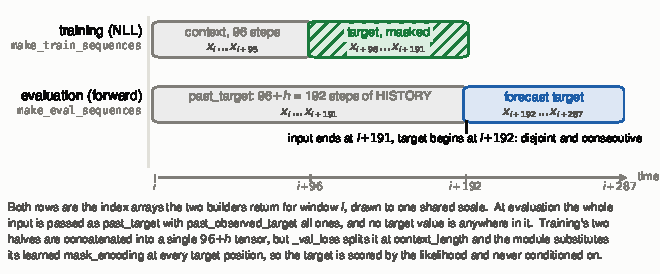
\includegraphics[width=\linewidth]{figA_window_layout.pdf}
\caption{\textbf{Which timesteps Moirai is given, and which it is asked to
predict}, at $h{=}96$; $h{=}192$ is the same layout with $h$ substituted.  Both
rows are the index arrays that \texttt{make\_train\_sequences} and
\texttt{make\_eval\_sequences} return for window~$i$, drawn to one shared scale.
At evaluation the model input is the $96{+}h$ steps \emph{preceding} the forecast
window and the target is the $h$ steps strictly after it: the two are disjoint and
consecutive, so no target value reaches the model.  The figure is generated from
those functions' output and asserts that disjointness at draw time.}
\label{fig:windowlayout}
\end{figure}

\textbf{Window construction, and exactly which values Moirai is given.}
The evaluation windows use an ``extended lookback'' of $96{+}h$ steps, which
could be read as though the forecast target were part of the model input.  It
is not, and because the training and evaluation window sets differ the
arithmetic is worth writing out.  Let $x_1,\dots,x_T$ be
the series and $h$ the horizon.  Both window sets are built by two
functions in \texttt{scripts/finetune\_forecasting.py}, named here so that
this paragraph and the code can be checked against each other.

\emph{Training} (\texttt{make\_train\_sequences}): window $i$ has context
$x_i,\dots,x_{i+95}$ and target $x_{i+96},\dots,x_{i+95+h}$.  The two are
concatenated into one $96{+}h$ tensor and passed to Moirai's
\texttt{\_val\_loss} with fixed patch size 32, which is the interface's
required calling convention: \texttt{\_val\_loss} splits the tensor at
\texttt{context\_length} and marks the latter part with
\texttt{prediction\_mask}, and the module then substitutes its learned
\texttt{mask\_encoding} at every masked position and zeroes the
corresponding observed flags.  The target values are therefore scored by
the likelihood and never conditioned on.

\emph{Evaluation} (\texttt{make\_eval\_sequences}): window $i$ has input
$x_i,\dots,x_{i+95+h}$ (that is, $96{+}h$ steps of \emph{history}),
and target $x_{i+96+h},\dots,x_{i+95+2h}$.  The input's last index is
$i+95+h$ and the target's first is $i+96+h$, so the two windows are
disjoint and consecutive and no target value appears anywhere in the model
input.  Only the input is passed, as \texttt{past\_target} with
\texttt{past\_observed\_target} all ones; the point prediction is the
median of 20 forecast samples with \texttt{patch\_size='auto'}.
``Extended lookback'' thus means a longer \emph{history}, not
history-plus-target.  Figure~\ref{fig:windowlayout} draws both layouts
from the index arrays those two functions actually return rather than from
this description, and asserts the disjointness at draw time, so the figure
cannot drift from the implementation.

The one asymmetry this does introduce is between models: Moirai is given
$96{+}h$ steps of history where the fitted baseline of
Appendix~\ref{app:gatecorrection} is given 96.  That direction favours the
pre-trained model (more context lowers $\text{MSE}_{\text{ZS}}$, raises
$\Vb{b}$ and so admits \emph{more} cells), and
Appendix~\ref{app:baselines:matchedlb} measures it rather than arguing it, by
giving the baseline the same $96{+}h$ history.

All data is fed to Moirai in raw scale (Moirai's internal
PackedStdScaler handles instance normalization); predictions and targets
are then normalized using training-set mean and standard deviation
for MSE/MAE computation, matching the standard time-series forecasting
evaluation protocol.

\textbf{Condition C's objective and its contrastive labels.}
Condition~B fine-tunes on NLL only; condition~C adds a supervised contrastive
term~\citep{khosla2020supcon},
$\mathcal{L}(\theta) = \mathcal{L}_{\text{NLL}}(\theta) +
\lambda\,\mathcal{L}_{\text{SupCon}}(\mathbf{z}, \mathbf{y};\, \tau)$, with
$\lambda = 0.5$ and $\tau = 0.07$.  Condition~C appears in this paper only as a
protocol variant of~B and carries no claim; the comparison every claim turns on
is B against~D.
For the contrastive labels we divide training sequences into
8 temporal clusters based on their position in the time series.
Sequences within the same cluster are positive pairs; sequences from
different clusters are negatives.
This encourages the encoder to maintain temporal-regime awareness.

\textbf{Horizon selection.}
We evaluate $h{=}96$ and $h{=}192$, the two horizons at which Moirai-Small on
ETTh2 clears the value gate: measured against the fitted lookback-96 baseline
the gate is defined with (Appendix~\ref{app:gatecorrection}),
$\Vb{\text{ridge}}{=}{+}0.400$ at $h{=}96$ and ${+}0.464$ at
$h{=}192$ on held-out windows.
Horizons $h{=}336$ and $h{=}720$ exceed Moirai-Small's
\texttt{max\_seq\_len}$=$512 constraint when combined with the
required extended lookback and are omitted.

% ============================================================
\section{ETTh2 Drift Diagnosis and Mitigation (Full Tables)}
\label{app:full_tables}
% ============================================================

This section contains the full tables referenced in \S\ref{sec:forecasting}.
Table~\ref{tab:mitigation_spectrum} shows the mitigation spectrum, conditions~B
through~H on Moirai-Small/ETTh2 at both horizons.

% GENERATED by scripts/emit_r2task.py from results/gate_val_side.json and results/gate_test_side.json -- do not hand-edit.
% The corrected fitted-baseline gate: scripts/gate_all_cells.py --baseline fitted, on both
% splits (300 matched selection windows, 300 matched held-out windows).
% Superseded trend-baseline values are preserved in
% results/gate_test_side_trend.json / results/gate_val_side_trend.json and are not read here.
\begin{table}[t]
\centering
\caption{Baseline-relative pre-trained advantage $\Vb{\text{ridge}} {=} 1 {-}
\text{MSE}_{\text{ZS}}/\text{MSE}_{\text{Linear}}$ for every Moirai cell, on both
splits. The \emph{selection} columns are the paper's primary gate: they are disjoint from
the held-out windows every intervention outcome is scored on, so cell inclusion is not a
judgement made after seeing the outcome. The \emph{held-out} columns are the retrospective
variant, reported as a sensitivity analysis. Bold marks a pass on the \emph{primary} split
in both columns of that row, so the bold set is the one the body's counts refer to.
\textbf{Not a linear probe}: this is a ratio of forecast MSEs computed through
Moirai's own forecasting head, and shares no machinery with a
linear-probe $\Delta R^2$ axis.
\textbf{Estimator, exactly}: $\text{MSE}_{\text{ZS}}$ is the median of 20
Moirai forecast samples at extended lookback (context $+$ horizon);
$\text{MSE}_{\text{Linear}}$ is a single lookback-96 ridge-OLS linear map
$\mathbb{R}^{96 \times D} {\to} \mathbb{R}^{h \times D}$ \emph{fit on the
cell's training windows} and applied unchanged out of sample; both are computed
on the same matched windows within a split (300 selection, 300
held-out), train-normalised.
The gate involves no fine-tuning, so a cell has one value at every $n$: the
$n{=}500$ and $n{=}10$k (ES) operating points reported in
\S\ref{sec:forecasting} share the entry shown here.
Bold ${=}$ gate-pass at the $0.20$ threshold on the primary split. ``---'' ${=}$ not run.}
\label{tab:r2task}
\small
\begin{tabular}{ll cc cc}
\toprule
& & \multicolumn{2}{c}{Selection (primary)} & \multicolumn{2}{c}{Held-out (retrosp.)} \\
\cmidrule(lr){3-4}\cmidrule(lr){5-6}
Backbone & Dataset & $h{=}96$ & $h{=}192$ & $h{=}96$ & $h{=}192$ \\
\midrule
\multicolumn{6}{l}{\textit{Moirai-Small}} \\
 & ETTh1                  & $-$0.177 & $-$0.347 & $-$0.243 & $-$0.331 \\
 & ETTh2                  & $\mathbf{+0.874}$ & $\mathbf{+0.932}$ & $\mathbf{+0.400}$ & $\mathbf{+0.464}$ \\
 & ETTm2                  & $-$0.164 & $\mathbf{+0.352}$ & $-$0.110 & $\mathbf{+0.108}$ \\
 & Weather                & $-$0.546 & $-$0.506 & $-$0.867 & $-$0.639 \\
 & \texttt{Electricity7}  & $-$0.650 & $-$0.455 & $-$0.085 & $-$0.047 \\
\midrule
\multicolumn{6}{l}{\textit{Moirai-Base}} \\
 & ETTh1                  & $-$0.312 & $-$0.600 & $-$0.458 & $-$0.501 \\
 & ETTh2                  & $\mathbf{+0.777}$ & $\mathbf{+0.925}$ & $\mathbf{+0.361}$ & $\mathbf{+0.275}$ \\
 & ETTm2                  & $-$0.257 & $\mathbf{+0.211}$ & $-$0.057 & $\mathbf{+0.083}$ \\
 & Weather                & $-$0.823 & $-$0.633 & $-$1.029 & $-$1.324 \\
\midrule
\multicolumn{6}{l}{\textit{Moirai-Large}} \\
 & ETTh1                  & $-$0.248 & --- & $-$0.454 & --- \\
 & ETTh2                  & $\mathbf{+0.875}$ & --- & $\mathbf{+0.219}$ & --- \\
 & Weather                & $-$0.638 & --- & $-$0.621 & --- \\
\bottomrule
\end{tabular}
\vspace{1pt}

{\footnotesize
\textbf{Reading:} seven of these 21 cells clear the $0.20$ threshold on the selection windows and five on the held-out windows.
The selection set contains the held-out set and adds two (ETTm2, ETTm2), so the retrospective variant is the stricter of the two here.
The primary survivors span two datasets: ETTh2, ETTm2.
$\Vb{\text{ridge}}{<}0$ means the linear baseline wins outright.
Appendix~\ref{app:gatecorrection} compares these against an unfitted
per-window trend baseline.
\texttt{Electricity7} is Electricity restricted to 7 of its 370 series (six
\texttt{MT} series plus \texttt{OT}), a deliberate protocol deviation that
keeps the cell dimensionality-matched to ETT/Weather.}
\end{table}


Table~\ref{tab:sample_sweep} gives the sample-size sweep on ETTh2
($h{=}96$, condition~B) referenced in \S\ref{sec:exp3}.

% GENERATED by scripts/emit_sample_sweep.py -- do not edit by hand.
\begin{table}[t]
\centering
\caption{\textbf{Sample-size sweep on Moirai-Small/ETTh2} ($h{=}96$, condition~B).
On held-out windows drift grows (CKA$\downarrow$ as $n\uparrow$) while forgetting
\emph{falls}: more data moves the encoder further and leaves the model further ahead
of zero-shot ($10/10$ seeds negative at $n{=}10{,}000$, Wilson CI
$[0.72, 1.00]$).  \textbf{If drift magnitude predicted harm the two columns
would rise together; they move in opposite directions.}  Scored on the selection
windows instead (\emph{sel.}), forgetting is non-monotonic in $n$, the
selection-split effect of \S\ref{sec:analysis:heldout}.
Dispersion here is the sample standard deviation over seeds
($\text{ddof}{=}1$), not the standard error the rest of the paper reports,
because the table is about how the spread across seeds moves with $n$.}
\label{tab:sample_sweep}
\small
\begin{tabular}{@{}rrcccc@{}}
\toprule
Samples & $k$ & held-out MSE & Forg.\% & Forg.\% (sel.) & CKA \\
\midrule
500 & 3 & .518{\tiny$\pm$.096} & +5.2{\tiny$\pm$19.5} & +14.0{\tiny$\pm$6.7} & .949{\tiny$\pm$.010} \\
1{,}000 & 3 & .461{\tiny$\pm$.019} & $-$6.4{\tiny$\pm$3.8} & +13.4{\tiny$\pm$9.1} & .936{\tiny$\pm$.025} \\
2{,}000 & 3 & .429{\tiny$\pm$.019} & $-$12.8{\tiny$\pm$3.8} & $-$2.9{\tiny$\pm$5.9} & .814{\tiny$\pm$.042} \\
5{,}000 & 7 & .401{\tiny$\pm$.015} & $-$18.5{\tiny$\pm$3.0} & +6.6{\tiny$\pm$10.0} & .546{\tiny$\pm$.082} \\
10{,}000$^{\mathrm{cuda}}$ & 10 & .401{\tiny$\pm$.044} & $-$18.5{\tiny$\pm$8.8} & $-$5.3{\tiny$\pm$6.6} & .518{\tiny$\pm$.199} \\
\bottomrule
\end{tabular}

\smallskip
{\footnotesize
$^{\mathrm{cuda}}$The $n{=}10{,}000$ row is the CUDA arm (A10G): 10 deterministic seeds, 10 epochs \emph{with} early
stopping (mean best epoch $4.2{\pm}1.3$).  Every
smaller $n$ is MPS, 20 epochs \emph{without} early stopping.  That is the
protocol difference Table~\ref{tab:trainers} lists;
Appendix~\ref{app:limitations}~(2) gives the $n{=}10{,}000$ seeds and the
matched MPS comparisons.
Rows read \texttt{test\_mse}, \texttt{forgetting\_pct} and
\texttt{final\_cka} from the per-run records in
\texttt{results/v8\_final/n\{500,1000,2000,5000\}},
\texttt{results/v9\_n5k\_seeds} and
\texttt{results/v19\_cuda\_etth2\_n10k}.}
\end{table}


\paragraph{The full 31-cell intervention evidence base.}
Table~\ref{tab:heldout_all} lists every cell carrying a paired B/D
intervention behind the headline claim of \S\ref{sec:intro}: 31 of the 32
screened cells, the screen itself being a gate value and needing no
intervention run: three backbones, six datasets, three Moirai capacities and
two horizons, each with its selection-split gate and the intervention contrast
B$-$D (positive ${=}$ the frozen encoder was better). It is generated by
\texttt{scripts/cell\_matrix.py --latex} directly from the committed run
JSON; no value in it is transcribed by hand. The two protocol arms
(\S\ref{sec:forecasting} at $h{=}96/192$, \S\ref{sec:forecasting:nonmoirai}
at $h{=}24$) are listed together for completeness but are never pooled into a
single statistic.

\begin{table}[ht]
\centering
\caption{All 31 intervention cells (the 31 of 32 screened cells with a paired
B/D run): \textbf{selection-split} gate $\Vb{\text{ridge}}$ (the primary gate of
\S\ref{sec:forecasting:gate}, scored on windows disjoint from the outcome columns
beside it), then
B$-$D on validation and on held-out windows (positive ${=}$ the frozen
encoder was better), and whether the validation and held-out readings
disagree in sign. Every row names its own $n$ because $n$ is \emph{not}
constant down the column: the ETTh2 spectrum cells ran at 500 while their
same-dataset neighbours ran at 1{,}000, and a row that stayed silent would read
as sharing its neighbour's. ILI is the one cell with no cap: it trains on its
whole 452-window split, since it is the only series small enough, so its
$n$ is a size rather than a subsample. Generated by
\texttt{scripts/cell\_matrix.py --latex}.}
\label{tab:heldout_all}
% GENERATED by scripts/cell_matrix.py --latex -- do not edit by hand.
\begin{center}
\small
\setlength{\tabcolsep}{4pt}
\begin{tabular}{@{}lccccc@{}}
\toprule
Cell & Seeds & Gate $\Vb{\text{ridge}}$ & B$-$D validation & B$-$D held-out & Reverses? \\
\midrule
Chronos / ETTh1 ($h{=}24$, $n{=}$8000) & 3 & $-0.116$\,\textsuperscript{f} & $+6.8{\pm}2.9$ & $\mathbf{-39.2{\pm}13.9}$ & yes \\
Moirai-S / ILI ($h{=}24$, $n{=}$452) & 10 & $-10.206$\,\textsuperscript{f} & $-62.6{\pm}1.4$ & $\mathbf{-38.6{\pm}1.3}$ & no \\
Chronos / ETTm2 ($h{=}24$, $n{=}$8000) & 3 & $-0.275$\,\textsuperscript{f} & $-24.1{\pm}9.8$ & $\mathbf{-29.5{\pm}6.4}$ & no \\
Moirai-B / ETTh2 ($h{=}96$, $n{=}$1000) & 3 & $+0.777$ & $+3.8{\pm}4.1$ & $\mathbf{-22.3{\pm}2.9}$ & yes \\
Chronos / Weather ($h{=}24$, $n{=}$8000) & 3 & $-0.203$\,\textsuperscript{f} & $-22.4{\pm}4.5$ & $\mathbf{-21.6{\pm}3.2}$ & no \\
Moirai-L / ETTh2 ($h{=}96$, $n{=}$500) & 3 & $+0.875$ & $+7.2{\pm}5.8$ & $\mathbf{-20.8{\pm}1.4}$ & yes \\
Moirai-B / ETTh2 ($h{=}192$, $n{=}$1000) & 3 & $+0.925$ & $-3.9{\pm}6.2$ & $\mathbf{-20.2{\pm}1.1}$ & no \\
Chronos / ETTh2 ($h{=}24$, $n{=}$8000) & 3 & $-0.184$\,\textsuperscript{f} & $-19.9{\pm}3.2$ & $\mathbf{-12.9{\pm}0.6}$ & no \\
TimesFM / ETTm2 ($h{=}24$, $n{=}$1000) & 3 & $+0.082$\,\textsuperscript{f} & $-12.2{\pm}12.4$ & $\mathbf{-7.7{\pm}2.6}$ & no \\
TimesFM / ETTh2 ($h{=}24$, $n{=}$1000) & 3 & $-0.208$\,\textsuperscript{f} & $+0.2{\pm}2.9$ & $\mathbf{-7.1{\pm}3.1}$ & yes \\
Moirai-S / Electricity7 ($h{=}96$, $n{=}$1000) & 3 & $-0.650$\,\textsuperscript{f} & $-10.4{\pm}1.1$ & $\mathbf{-3.2{\pm}1.5}$ & no \\
Chronos / Electricity ($h{=}24$, $n{=}$8000) & 3 & $-0.089$\,\textsuperscript{f} & $-10.3{\pm}3.2$ & $\mathbf{-2.7{\pm}1.9}$ & no \\
Moirai-S / Electricity7 ($h{=}192$, $n{=}$1000) & 3 & $-0.455$\,\textsuperscript{f} & $-8.2{\pm}1.9$ & $\mathbf{-2.6{\pm}2.1}$ & no \\
TimesFM / Weather ($h{=}24$, $n{=}$1000) & 3 & $-0.160$\,\textsuperscript{f} & $-4.8{\pm}0.6$ & $\mathbf{-1.6{\pm}1.5}$ & no \\
TimesFM / ETTh1 ($h{=}24$, $n{=}$1000) & 3 & $-0.101$\,\textsuperscript{f} & $-5.4{\pm}0.9$ & $\mathbf{-1.4{\pm}2.8}$ & no \\
Moirai-B / ETTm2 ($h{=}192$, $n{=}$1000) & 3 & $+0.211$ & $+3.5{\pm}1.5$ & $\mathbf{+1.3{\pm}3.4}$ & no \\
Moirai-S / ETTm2 ($h{=}96$, $n{=}$1000) & 5 & $-0.164$\,\textsuperscript{f} & $+6.5{\pm}2.9$ & $\mathbf{+2.6{\pm}3.4}$ & no \\
Moirai-S / ETTh2 ($h{=}96$, $n{=}$500) & 10 & $+0.874$ & $+10.6{\pm}2.8$ & $\mathbf{+2.8{\pm}3.7}$ & no \\
Moirai-S / ETTm2 ($h{=}192$, $n{=}$1000) & 5 & $+0.352$ & $+8.6{\pm}3.3$ & $\mathbf{+4.7{\pm}3.2}$ & no \\
Moirai-S / ETTh2 ($h{=}192$, $n{=}$500) & 10 & $+0.932$ & $+17.4{\pm}4.3$ & $\mathbf{+6.1{\pm}3.4}$ & no \\
Moirai-B / ETTm2 ($h{=}96$, $n{=}$1000) & 3 & $-0.257$\,\textsuperscript{f} & $+3.9{\pm}3.7$ & $\mathbf{+7.0{\pm}2.4}$ & no \\
Moirai-B / Weather ($h{=}96$, $n{=}$1000) & 3 & $-0.823$\,\textsuperscript{f} & $+19.3{\pm}0.8$ & $\mathbf{+9.4{\pm}2.0}$ & no \\
Moirai-L / Weather ($h{=}96$, $n{=}$1000) & 3 & $-0.638$\,\textsuperscript{f} & $+4.3{\pm}6.5$ & $\mathbf{+12.0{\pm}7.5}$ & no \\
Moirai-B / Weather ($h{=}192$, $n{=}$1000) & 3 & $-0.633$\,\textsuperscript{f} & $+30.6{\pm}12.0$ & $\mathbf{+12.5{\pm}8.7}$ & no \\
Moirai-S / ETTh1 ($h{=}192$, $n{=}$1000) & 5 & $-0.347$\,\textsuperscript{f} & $+14.8{\pm}1.9$ & $\mathbf{+13.5{\pm}1.7}$ & no \\
Moirai-S / ETTh1 ($h{=}96$, $n{=}$1000) & 5 & $-0.177$\,\textsuperscript{f} & $+16.1{\pm}1.5$ & $\mathbf{+22.1{\pm}2.3}$ & no \\
Moirai-L / ETTh1 ($h{=}96$, $n{=}$1000) & 3 & $-0.248$\,\textsuperscript{f} & $+13.4{\pm}2.1$ & $\mathbf{+28.2{\pm}4.9}$ & no \\
Moirai-B / ETTh1 ($h{=}96$, $n{=}$1000) & 3 & $-0.312$\,\textsuperscript{f} & $+15.8{\pm}4.6$ & $\mathbf{+37.5{\pm}8.2}$ & no \\
Moirai-B / ETTh1 ($h{=}192$, $n{=}$1000) & 3 & $-0.600$\,\textsuperscript{f} & $+15.6{\pm}2.3$ & $\mathbf{+47.0{\pm}13.8}$ & no \\
Moirai-S / Weather ($h{=}96$, $n{=}$1000) & 3 & $-0.546$\,\textsuperscript{f} & $+55.4{\pm}4.3$ & $\mathbf{+53.1{\pm}10.2}$ & no \\
Moirai-S / Weather ($h{=}192$, $n{=}$1000) & 3 & $-0.506$\,\textsuperscript{f} & $+70.2{\pm}12.3$ & $\mathbf{+62.1{\pm}13.6}$ & no \\
\bottomrule
\end{tabular}
\end{center}

\end{table}


\begin{table}[ht]
\centering
\caption{\textbf{The four sign reversals between selection and held-out
windows} (\S\ref{sec:analysis:heldout}). $\Delta$ adapted and $\Delta$ frozen
are the change in each arm's forgetting when scoring moves from the selection
split to the held-out split; $\text{zs}_\text{test}/\text{zs}_\text{val}$ is
the untrained checkpoint's error ratio between the two splits, an
exchangeability check that involves no fine-tuning. All four reversals run from
``frozen better'' to ``adapted better''. $n$ is per row and not constant
(Table~\ref{tab:heldout_all}), and is taken from the published row rather than
re-read here. Generated by \texttt{scripts/heldout\_decomposition.py}.}
\label{tab:heldout_decomp}
% GENERATED by scripts/heldout_decomposition.py -- do not edit by hand.
\begin{center}
\small
\setlength{\tabcolsep}{4pt}
\begin{tabular}{@{}lccccc@{}}
\toprule
Cell & B$-$D val & B$-$D held-out & $\Delta$ adapted (B) & $\Delta$ frozen (D) & $\text{zs}_\text{test}/\text{zs}_\text{val}$ \\
\midrule
Chronos / ETTh1 ($h{=}24$, $n{=}$8000) & $+6.8$ & $-39.2$ & $+8.0$ & $+53.9$ & $0.98$ \\
Moirai-B / ETTh2 ($h{=}96$, $n{=}$1000) & $+3.8$ & $-22.3$ & $+12.2$ & $+38.3$ & $2.31$ \\
Moirai-L / ETTh2 ($h{=}96$, $n{=}$500) & $+7.2$ & $-20.8$ & $-52.9$ & $-24.8$ & $5.07$ \\
TimesFM / ETTh2 ($h{=}24$, $n{=}$1000) & $+0.2$ & $-7.1$ & $-11.7$ & $-4.3$ & $1.09$ \\
\bottomrule
\end{tabular}
\end{center}

\end{table}

\paragraph{Why the four reverse in one direction, and the two mechanisms behind it.}
\textbf{The four reversals of \S\ref{sec:analysis:heldout} do not share one per-arm
story.}  Normalising each arm by the zero-shot error on its own split is an identity
rather than a model, so the two arms' held-out-minus-selection moves account for the
reversal exactly.  On \textbf{two of the four} the frozen arm collapses out of sample
and the selection-optimism reading holds: Chronos/ETTh1 is the largest reversal in the
matrix at $+6.8$ on the selection windows against $-39.2$ held out, a $46.0$-point
swing ($\Delta$ frozen $+53.9$ against $\Delta$ adapted $+8.0$ on Chronos/ETTh1, the
largest of the four).  On the \textbf{other two} both arms finish \emph{better} than
their own zero-shot out of sample and nothing degrades at all --- the adapted arm
merely gains more --- so half the reversals are a different phenomenon wearing the
same sign change.  What all four share is not a mechanism but a location:
they concentrate where the two splits are least exchangeable: the
\emph{untrained} checkpoint's held-out-to-selection error ratio spans $0.98$ to
$5.07$ across these four cells, a quantity that involves no fine-tuning at all.  A
frozen encoder cannot adapt to that shift and a fine-tuned one partly can, which is
exactly the asymmetry that makes same-split scoring flatter freezing, so the
direction of the four reversals is not a coincidence to be noted but a consequence
to be expected, and it is why scoring $\denc$ on selection windows is not a
defensible option rather than merely a less careful one.


\begin{table}[ht]
\centering
\caption{\textbf{Cross-backbone results ($h{=}24$)}
(\S\ref{sec:forecasting:nonmoirai}). Every non-Moirai cell with a paired
frozen-encoder run: \textbf{selection-split} gate $\Vb{\text{ridge}}$
(\textsuperscript{f}${=}$gate-fail at the $0.20$ operating point; all nine
fail, as does the screened-only TimesFM/Electricity cell, which has no paired run
and so no selection-split gate: it scores $+0.132$ on the held-out windows), CKA
after full fine-tuning, and the two outcome readings as \% change against
zero-shot (\emph{negative is better than zero-shot}). \textbf{Protocol note:}
this arm is univariate OT, lookback 96, $h{=}24$, 200 held-out windows,
per-window $z$-scored; the Moirai arm of \S\ref{sec:forecasting} is lookback
192, $h{=}96$, 300 windows, train-normalised. Gates for both arms come from one
source (\texttt{results/gate\_val\_side.json}, via
\texttt{scripts/cell\_matrix.py}); the two arms are never pooled.}
\label{tab:crossbackbone}
% GENERATED by scripts/emit_crossbackbone.py -- do not edit by hand.
\begin{center}
\small
\setlength{\tabcolsep}{5pt}
\begin{tabular}{@{}llcccc@{}}
\toprule
Backbone & Dataset & Gate $\Vb{\text{ridge}}$ & CKA & Full FT & Frozen \\
\midrule
Chronos-T5-S & ETTm2 & $-0.275$\,\textsuperscript{f} & $0.112$ & $-41.4\%$ & $-11.9\%$ \\
Chronos-T5-S & Weather & $-0.203$\,\textsuperscript{f} & $0.092$ & $-5.7\%$ & $+15.9\%$ \\
Chronos-T5-S & Electricity & $-0.089$\,\textsuperscript{f} & $0.232$ & $-2.3\%$ & $+0.4\%$ \\
Chronos-T5-S & ETTh2 & $-0.184$\,\textsuperscript{f} & $0.094$ & $-0.4\%$ & $+12.5\%$ \\
Chronos-T5-S & ETTh1 & $-0.116$\,\textsuperscript{f} & $0.169$ & $+20.6\%$ & $+59.8\%$ \\
\midrule
TimesFM-2.5 & ETTm2 & $+0.082$\,\textsuperscript{f} & $0.360$ & $-51.8\%$ & $-44.1\%$ \\
TimesFM-2.5 & ETTh2 & $-0.208$\,\textsuperscript{f} & $0.246$ & $-20.4\%$ & $-13.3\%$ \\
TimesFM-2.5 & Weather & $-0.160$\,\textsuperscript{f} & $0.335$ & $-7.8\%$ & $-6.1\%$ \\
TimesFM-2.5 & ETTh1 & $-0.101$\,\textsuperscript{f} & $0.561$ & $-3.0\%$ & $-1.6\%$ \\
\bottomrule
\end{tabular}
\end{center}

\end{table}


\paragraph{The mitigation spectrum, cell by cell.}
Table~\ref{tab:mitigation_spectrum} reports five strategies spanning
unconstrained fine-tuning to full freezing, all on Moirai/ETTh2. The body
(\S\ref{sec:exp3}) states only the conclusion; the per-method
readings are here. \textbf{LoRA} ($r{=}8$, $\alpha{=}16$) improves over
zero-shot at $h{=}96$ at CKA $0.979$, but is not uniformly safe: on
Moirai-Large it fails at the default learning rate ($+25.7\%$) and only a
$10\times$ LR reduction rescues it ($-8.5\%$, CKA $0.989$), so tune the
learning rate before the rank (Appendix~\ref{app:lora_rank}). \textbf{EWC and
L2-SP} reduce drift without buying utility: at $n{=}1{,}000$, $h{=}96$, each
scored against its own zero-shot, they land at $+13.4$ to $+16.0\%$, against the
$+11.1\%$ full fine-tuning reaches at $n{=}500$.  Those two figures are not
matched on training-set size (no full-fine-tuning arm at $n{=}1{,}000$ on this
cell has more than a single seed), so what we read off them is that anchoring
buys no utility, not an ordering between anchoring and full fine-tuning. \textbf{Freezing} eliminates drift but cannot adapt, and the
strict freeze of Appendix~\ref{app:strictfreeze} shows that even the residual
adaptation condition~D permits is doing work. The screen is what makes this
spectrum hard to act on: none of these methods has a demonstrated advantage to
protect on 27 of our 32 cells, and on three of the remaining five the
unconstrained condition beats both of the others run there: zero-shot by
$31$--$42\%$ and the frozen encoder by $20$--$22$ points.

\textbf{Condition coverage differs by cell, and we state it rather than let the
widest row imply it.} The full six-condition comparison exists only for
Moirai-Small/ETTh2, so ``best of six'' is not a claim available for any other
cell. Every intervention cell has B and D. Condition~H (strict freeze) adds 16
cells (Appendix~\ref{app:strictfreeze}) and condition~E (LoRA) adds 8
(Appendix~\ref{app:loravaluecells}), both on the seeds given in their own tables;
L2-SP and EWC exist on Moirai-Small/ETTh2 alone. A claim about a cell is
therefore a claim about the conditions that cell ran, and the per-cell seed
counts are printed in every table rather than summarised into one figure.

% GENERATED by scripts/emit_mitigation_spectrum.py -- do not edit by hand.
\begin{table}[t]
\centering
\caption{\textbf{Mitigation spectrum on Moirai-Small/ETTh2.}
Rows ordered by representation preservation (CKA at $h{=}96$).
On \emph{this} cell LoRA preserves representations (CKA${\approx}0.98$) while
\emph{improving} on zero-shot, and weight anchoring reduces drift without buying
utility.  \textbf{Neither reading generalises, and we checked rather than assumed:}
extending condition~E to 8 further value-cells
(Appendix~\ref{app:loravaluecells}) puts CKA$_\text{E}$ anywhere from $0.55$ to
$0.97$ and leaves full fine-tuning ahead of LoRA on 4 of the 8.
\textbf{Every row is scored against its own zero-shot.} Forgetting\% is the
mean over seeds of each run's $(\text{fine-tuned}-\text{zero-shot})/
\text{zero-shot}$, so no row borrows another's denominator.  MSE, CKA and $\ell_2$ drift are means over
seeds with population std (ddof${=}0$); the body's SEM convention
(\S\ref{sec:method}) does not apply here.
\textbf{The rows are not matched on training-set size.}
Conditions B, C and D use $n{=}500$ training samples (zero-shot MSE $.1256$ at $h{=}96$, $.1580$ at $h{=}192$);
E, F and G use $n{=}1{,}000$ (zero-shot MSE $.1274$ and $.1596$); the two rightmost
columns give the seed count and the training-set size separately.
We therefore claim no ordering \emph{between} the two
groups: there is no full-fine-tuning arm at $n{=}1{,}000$ on this cell with more
than a single seed, so ``anchoring ties full fine-tuning'' is not a comparison
these runs support.  The dissociation the table is cited for (CKA not predicting
utility) is within-group and unaffected.
Condition~D reads CKA $0.99996$ rather than $1$: it leaves \texttt{in\_proj} and
\texttt{mask\_encoding} trainable, so it is a frozen-\emph{encoder} control and not
a strict freeze.  Only condition~H (Appendix~\ref{app:strictfreeze}) is $1.0000$ by
construction.}
\label{tab:mitigation_spectrum}
\small
\resizebox{\textwidth}{!}{%
\begin{tabular}{l cccc cccc cc}
\toprule
& \multicolumn{4}{c}{$h=96$} & \multicolumn{4}{c}{$h=192$} & & \\
\cmidrule(lr){2-5} \cmidrule(lr){6-9}
Method & MSE & Forg.\% & CKA & Drift & MSE & Forg.\% & CKA & Drift & seeds & $n$ \\
\midrule
B: Full fine-tune & .140{\tiny$\pm$.014} & $+$11.1 & .937{\tiny$\pm$.028} & 3.96{\tiny$\pm$.56} & .183{\tiny$\pm$.020} & $+$15.7 & .970{\tiny$\pm$.009} & 4.12{\tiny$\pm$.32} & 10 & 500 \\
F: L2-SP ($\lambda{=}0.01$) & .150{\tiny$\pm$.006} & $+$16.0 & .939{\tiny$\pm$.023} & 4.98{\tiny$\pm$.34} & .179{\tiny$\pm$.009} & $+$12.7 & .945{\tiny$\pm$.007} & 4.84{\tiny$\pm$.22} & 3 & 1{,}000 \\
C: NLL+SupCon & .138{\tiny$\pm$.010} & $+$10.1 & .949{\tiny$\pm$.014} & 3.72{\tiny$\pm$.43} & .178{\tiny$\pm$.011} & $+$12.9 & .964{\tiny$\pm$.015} & 3.97{\tiny$\pm$.34} & 10 & 500 \\
F: L2-SP ($\lambda{=}0.1$) & .147{\tiny$\pm$.003} & $+$13.4 & .965{\tiny$\pm$.006} & 2.94{\tiny$\pm$.08} & .181{\tiny$\pm$.003} & $+$13.6 & .980{\tiny$\pm$.002} & 2.84{\tiny$\pm$.02} & 3 & 1{,}000 \\
G: EWC ($\lambda{=}1000$) & .149{\tiny$\pm$.015} & $+$14.9 & .972{\tiny$\pm$.004} & 3.29{\tiny$\pm$.79} & .188{\tiny$\pm$.004} & $+$18.3 & .978{\tiny$\pm$.006} & 4.46{\tiny$\pm$.38} & 3 & 1{,}000 \\
E: LoRA ($r{=}8$)\textsuperscript{$\dagger$} & \textbf{.116}{\tiny$\pm$.001} & \textbf{$-$9.1} & .979{\tiny$\pm$.006} & 0.00{\tiny$\pm$.00} & \textbf{.157}{\tiny$\pm$.002} & \textbf{$-$1.8} & .986{\tiny$\pm$.005} & 0.00{\tiny$\pm$.00} & 5 & 1{,}000 \\
\midrule
D: Frozen encoder & .126{\tiny$\pm$.006} & $+$0.5 & .99996{\tiny$\pm$.00001} & 1.11{\tiny$\pm$.15} & .155{\tiny$\pm$.002} & $-$1.7 & .99995{\tiny$\pm$.00002} & 1.30{\tiny$\pm$.18} & 10 & 500 \\
\bottomrule
\end{tabular}%
}

\smallskip
{\footnotesize $\dagger$ LoRA ($\alpha{=}16$) adds low-rank updates that do not
modify base encoder parameters; $\ell_2$ drift is exactly zero by construction.}
\end{table}


\begin{figure}[t]
\centering
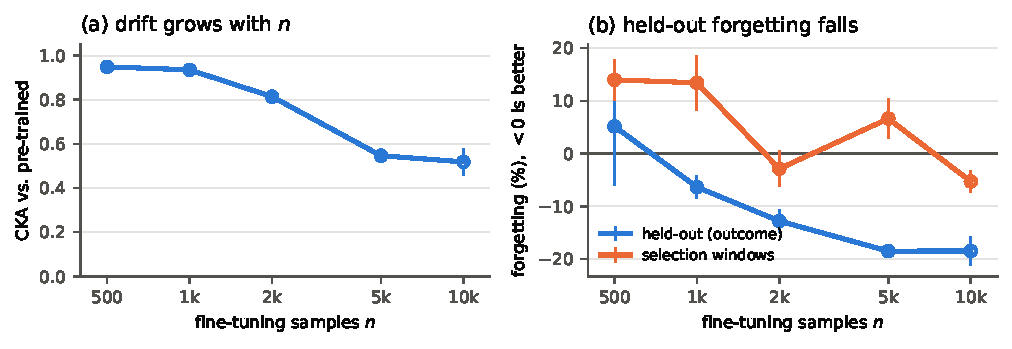
\includegraphics[width=\linewidth]{figures/dissociation_trajectory.pdf}
\caption{Sample-size sweep on Moirai-Small/ETTh2 (full fine-tuning, $h{=}96$),
read from the same records as Table~\ref{tab:sample_sweep}; error bars are
standard errors over seeds.  (a)~CKA against the pre-trained encoder falls as
$n$ grows.  (b)~Held-out forgetting falls with it, so more drift goes with a
better outcome; scored on the selection windows instead, forgetting is
non-monotonic.  Hollow markers at $n{=}10$k are the early-stopped arm.}
\label{fig:dissociation}
\end{figure}

% ============================================================
\section{The Strict-Freeze Control}
\label{app:strictfreeze}
% ============================================================

% Added 20 Sep 2026: a reviewer asked where exactly the freeze boundary falls, which the paragraph
% below states in words and four module names. The grid is transcribed from finetune_forecasting.py's
% requires_grad blocks by figA_freeze_boundary.py, which also asserts H's CKA is exactly 1 from the
% run records -- so the figure fails rather than misleads if the training code's freeze logic changes.
\begin{figure}[t]
\centering
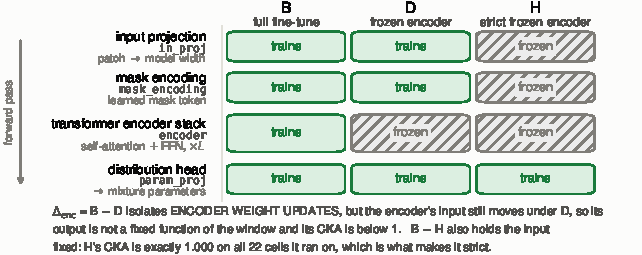
\includegraphics[width=\linewidth]{figA_freeze_boundary.pdf}
\caption{\textbf{Where the freeze boundary falls, module by module.} Green boxes are
parameters the optimiser may move; hatched boxes are held at their pre-trained
values.  The grid is transcribed from the \texttt{requires\_grad} assignments in
\texttt{scripts/finetune\_forecasting.py}.  Two of our seven survivors change the
sign of $\denc$ between~D and~H (Table~\ref{tab:strictfreeze}), so which of these
columns a paper means by ``we froze the encoder'' is not a detail.}
\label{fig:freezeboundary}
\end{figure}

Condition~D freezes the encoder's own weights but leaves the input projection
(\texttt{in\_proj}, $247{,}680$ parameters) and \texttt{mask\_encoding} ($384$)
trainable alongside the distribution head (\texttt{param\_proj},
$2{,}956{,}800$). What the encoder \emph{receives} therefore keeps changing, so
its output is not a fixed function of the input, which is why D's measured CKA
is $0.76$--$0.90$ on ILI and $0.97$--$0.99$ on Moirai-Base rather than
$1.000$. A reader can reasonably object that wherever ``freezing wins'', it
wins partly by re-fitting the input projection rather than by holding the
encoder still.

Condition~\textbf{H} removes the objection: \texttt{in\_proj} and
\texttt{mask\_encoding} are frozen too, so only \texttt{param\_proj} trains and
the encoder's output is pinned by construction (measured CKA $1.0000$ exactly,
as it must be). B$-$H is then a clean read of what allowing \emph{any}
encoder-side change was worth, and B$-$D versus B$-$H separates encoder
adaptation from input re-fitting. We fixed the reading rule before running: the
claim is that the sign and reading of B$-$D survive strict freezing, so B$-$H
is reported beside B$-$D on every cell, and divergence on any cell is reported
as that cell's gap being partly input re-fitting rather than being buried.

\textbf{Result} (Table~\ref{tab:strictfreeze}). The sixteen cells fall into
three groups. Seven were chosen before the gate was corrected: they are the six
that met the degradation
definition under the unfitted trend baseline
(Appendix~\ref{app:gatecorrection}), plus ILI. Nothing was dropped; two cells
the prospective arm later added (Moirai-Large on ETTh1 and on Weather) postdate
this control and carry no H run. That selection no longer picks out a privileged
class (against the fitted baseline no cell meets the definition), but it
remains the set chosen to be \emph{most} favourable to the degradation story,
which is the useful property here. Five are the gate-passing
survivors of \S\ref{sec:forecasting:results}, run afterwards precisely because
the first seven did not reach them: until they existed, the survivors' readings
rested on condition~D alone. The last four are the Moirai/ETTm2 cells that clear
the screen against a rung other than the fitted line
(Appendix~\ref{app:valueaxis}), added so that the control covers value-cells
outside ETTh2: all four of them, at three seeds each, so ETTm2 is covered
completely rather than partially. Measured CKA is
$1.0000$ everywhere, confirming the construction.

\textbf{On twelve of the sixteen the reading survives; on four it reverses, and
the four are the ones we added.} B$-$H keeps B$-$D's sign on the original seven
and on the five survivors. There the magnitude
changes by $-13.1$ to $+28.9$~pp, and on the original seven by $-5.8$ to
$+0.5$~pp, so at most $5.8$~pp of a gap as large as
$62$~pp is input-projection re-fitting. On ILI, where adaptation helps, strict
freezing makes adaptation look \emph{more} valuable ($-38.6 \to -43.6$), which
is the same direction: holding more of the model still costs more where the
encoder was earning its keep. B$-$D is averaged over the seeds condition H
ran, so Moirai-Small/ETTh1's entries here are 3-seed values against the 5-seed
values quoted in Table~\ref{tab:heldout_all}.

\textbf{All four ETTm2 cells diverge, and we said in advance how that would be
read.} On every one of them $\denc$ changes sign between the two controls:
Moirai-Small $h{=}96$ goes from B$-$D $+7.3{\pm}2.9$ to B$-$H $-6.8{\pm}2.0$,
Moirai-Base $h{=}96$ from $+7.0{\pm}2.4$ to $-9.2{\pm}3.1$, Moirai-Small
$h{=}192$ from $+4.2{\pm}5.8$ to $-2.7{\pm}6.1$ and Moirai-Base $h{=}192$ from
$+1.3{\pm}3.4$ to $-2.4{\pm}2.9$: shifts of $-14.2$, $-16.2$, $-6.9$ and
$-3.7$~pp. The last of those is the weakest of the four and we do not lean on it:
both of its intervals straddle zero, so what that cell shows is a shift in the
mean and not a resolved reversal. The pattern is carried by the two $h{=}96$
cells, where the shift is four to five times the SEM. The consistency of the
\emph{direction} across all four is what the reading rests on: four cells, one
dataset, four shifts, all negative. The rule fixed before the runs was that divergence means part of
that cell's gap is input re-fitting, and that is what these say: on ETTm2,
condition~D's apparent ``freezing wins'' was carried \emph{entirely} by the
input projection adapting to the target, and once it is held fixed too,
allowing the encoder to adapt is the better choice. Two readings follow, and
they point the same way as the rest of the paper rather than against it. First,
the direction of the correction is towards adaptation on every diverging cell,
so nothing here recovers a degradation case; ETTm2 joins ETTh2 in the column
where full fine-tuning wins under the strict control. Second, and more
important for \S\ref{sec:exp2}, it is direct evidence that
\textbf{condition~D does not measure encoder adaptation alone}: on four of the
sixteen cells where we can separate the two, the loose control's sign is set by
the projections rather than by the encoder. That is a limit on B$-$D as an
estimand, and it is why \S\ref{sec:method} defines $\denc$ against the control
actually used and reports H beside it rather than substituting one for the
other.

\textbf{On the five survivors the control cuts against freezing, not for it.}
These are the cells the objection mattered most for, and on the three where full
fine-tuning already won, strict freezing \emph{widens} its margin rather than
narrowing it: B$-$D of $-22.3$, $-20.2$ and $-20.8$ becomes B$-$H of $-28.0$,
$-31.8$ and $-33.9$ on Moirai-Base $h{=}96$, Base $h{=}192$ and Large $h{=}96$,
a move of $-5.6$ to $-13.1$~pp. Part of what condition~D was scoring on these
cells was therefore the input projection re-fitting to the target data, and
removing it makes encoder adaptation look \emph{more} valuable, not less. On
Moirai-Small $h{=}192$ (the cell that comes closest to degradation), B$-$H is
$+1.2{\pm}8.5$ against B$-$D's $+4.1{\pm}8.6$: freezing still reads as better,
by less, with a standard error several times the mean either way. Condition~H
also improves on the un-tuned model in every seed of all five
(forg$_\text{H}$ from $-0.2\%$ to $-8.5\%$), so on the survivors both parts of
the degradation definition behave the same way under the strict control as
under the loose one.

\textbf{The one large change is the diverged seed.} Moirai-Small/ETTh2 $h{=}96$ moves from B$-$D $+13.7$ to
B$-$H $+42.6{\pm}29.5$, the only cell whose magnitude shifts by more than
$13$~pp. It is seed 42, which \S\ref{sec:forecasting:results} reports as a
training failure rather than an encoder-drift effect: that seed diverges under
full fine-tuning ($+98.9\%$) \emph{and} under the frozen encoder ($+91.1\%$),
but it cannot diverge under condition~H, where only \texttt{param\_proj} trains
and the run therefore sits at zero-shot ($-0.1\%$). Over the other two seeds
B$-$H is $+14.4$ against B$-$D's $+16.7$. The strict control thus supplies
independent support for the seed-42 diagnosis: what fails on that seed is
optimisation, and holding the encoder's \emph{inputs} fixed as well as its
weights is what prevents it.

\begin{table}[ht]
\centering
\caption{The strict-freeze control (condition~H) beside condition~D on sixteen
cells: the six that met the degradation definition under the unfitted trend
baseline, plus ILI, plus the five gate-passing survivors of
\S\ref{sec:forecasting:results}, plus all four Moirai/ETTm2 value-cells.
\textbf{B$-$H keeps B$-$D's sign on twelve and reverses it on all four ETTm2
cells}, where condition~D's margin was the input projection re-fitting rather
than the encoder being held still. B$-$D is restricted to the seeds condition~H
ran, and a cell with fewer than three H seeds is excluded and named by the
emitter rather than printed thin. $n$ is shown on every row and is not constant
down the column; ILI's $452$ is its whole training split rather than a cap
(Table~\ref{tab:heldout_all}). Generated by
\texttt{scripts/cell\_matrix.py --latex}.}
\label{tab:strictfreeze}
% GENERATED by scripts/cell_matrix.py --latex -- do not edit by hand.
\begin{center}
\small
\setlength{\tabcolsep}{5pt}
\begin{tabular}{@{}lccccc@{}}
\toprule
Cell & Seeds & B$-$D & B$-$H & forg$_\text{H}$ & CKA$_\text{H}$ \\
\midrule
Moirai-S / Weather ($h{=}192$, $n{=}$1000) & 3 & $+62.1{\pm}13.6$ & $\mathbf{+56.7{\pm}13.5}$ & $-10.6{\pm}0.3$ & $1.0000$ \\
Moirai-S / Weather ($h{=}96$, $n{=}$1000) & 3 & $+53.1{\pm}10.2$ & $\mathbf{+50.1{\pm}6.6}$ & $-12.8{\pm}0.6$ & $1.0000$ \\
Moirai-B / ETTh1 ($h{=}192$, $n{=}$1000) & 3 & $+47.0{\pm}13.8$ & $\mathbf{+47.5{\pm}13.7}$ & $-8.0{\pm}0.4$ & $1.0000$ \\
Moirai-B / ETTh1 ($h{=}96$, $n{=}$1000) & 3 & $+37.5{\pm}8.2$ & $\mathbf{+32.5{\pm}8.2}$ & $-9.7{\pm}0.4$ & $1.0000$ \\
Moirai-L / ETTh1 ($h{=}96$, $n{=}$1000) & 3 & $+28.2{\pm}4.9$ & $\mathbf{+24.9{\pm}5.0}$ & $-10.9{\pm}0.7$ & $1.0000$ \\
Moirai-S / ETTh1 ($h{=}96$, $n{=}$1000) & 3 & $+23.2{\pm}3.6$ & $\mathbf{+20.4{\pm}3.6}$ & $-0.6{\pm}0.2$ & $1.0000$ \\
Moirai-S / ETTh1 ($h{=}192$, $n{=}$1000) & 3 & $+14.5{\pm}1.4$ & $\mathbf{+8.7{\pm}1.5}$ & $+1.2{\pm}0.4$ & $1.0000$ \\
Moirai-S / ETTh2 ($h{=}96$, $n{=}$500) & 3 & $+13.7{\pm}9.0$ & $\mathbf{+42.6{\pm}29.5}$ & $-0.2{\pm}0.1$ & $1.0000$ \\
Moirai-B / Weather ($h{=}192$, $n{=}$1000) & 3 & $+12.5{\pm}8.7$ & $\mathbf{+4.1{\pm}7.2}$ & $-22.2{\pm}0.4$ & $1.0000$ \\
Moirai-L / Weather ($h{=}96$, $n{=}$1000) & 3 & $+12.0{\pm}7.5$ & $\mathbf{+11.0{\pm}6.4}$ & $-3.1{\pm}0.0$ & $1.0000$ \\
Moirai-B / Weather ($h{=}96$, $n{=}$1000) & 3 & $+9.4{\pm}2.0$ & $\mathbf{+0.5{\pm}2.5}$ & $-12.1{\pm}0.1$ & $1.0000$ \\
Moirai-S / ETTm2 ($h{=}96$, $n{=}$1000) & 3 & $+7.3{\pm}2.9$ & $\mathbf{-6.8{\pm}2.0}$ & $-2.9{\pm}0.4$ & $1.0000$ \\
Moirai-B / ETTm2 ($h{=}96$, $n{=}$1000) & 3 & $+7.0{\pm}2.4$ & $\mathbf{-9.2{\pm}3.1}$ & $-3.9{\pm}1.8$ & $1.0000$ \\
Moirai-S / ETTm2 ($h{=}192$, $n{=}$1000) & 3 & $+4.2{\pm}5.8$ & $\mathbf{-2.7{\pm}6.1}$ & $+1.3{\pm}0.3$ & $1.0000$ \\
Moirai-S / ETTh2 ($h{=}192$, $n{=}$500) & 3 & $+4.1{\pm}8.6$ & $\mathbf{+1.2{\pm}8.5}$ & $-1.4{\pm}0.2$ & $1.0000$ \\
Moirai-B / ETTm2 ($h{=}192$, $n{=}$1000) & 3 & $+1.3{\pm}3.4$ & $\mathbf{-2.4{\pm}2.9}$ & $-6.0{\pm}0.4$ & $1.0000$ \\
Moirai-S / Electricity7 ($h{=}192$, $n{=}$1000) & 3 & $-2.6{\pm}2.1$ & $\mathbf{-5.4{\pm}2.2}$ & $-13.2{\pm}0.1$ & $1.0000$ \\
Moirai-S / Electricity7 ($h{=}96$, $n{=}$1000) & 3 & $-3.2{\pm}1.5$ & $\mathbf{-5.2{\pm}2.0}$ & $-10.9{\pm}0.3$ & $1.0000$ \\
Moirai-B / ETTh2 ($h{=}192$, $n{=}$1000) & 3 & $-20.2{\pm}1.1$ & $\mathbf{-31.8{\pm}1.0}$ & $-4.5{\pm}2.0$ & $1.0000$ \\
Moirai-L / ETTh2 ($h{=}96$, $n{=}$500) & 3 & $-20.8{\pm}1.4$ & $\mathbf{-33.9{\pm}0.1}$ & $-8.5{\pm}0.5$ & $1.0000$ \\
Moirai-B / ETTh2 ($h{=}96$, $n{=}$1000) & 3 & $-22.3{\pm}2.9$ & $\mathbf{-28.0{\pm}3.3}$ & $-3.5{\pm}0.4$ & $1.0000$ \\
Moirai-S / ILI ($h{=}24$, $n{=}$452) & 10 & $-38.6{\pm}1.3$ & $\mathbf{-43.6{\pm}0.7}$ & $-7.1{\pm}0.5$ & $1.0000$ \\
\bottomrule
\end{tabular}
\end{center}

\end{table}

\textbf{One clause does not survive, and it is not the headline one.}
``Degradation'' has two parts: fine-tuning ends up worse than the un-tuned
model, \emph{and} freezing improves on it. The first part is a property of
condition B and is untouched by this control. The second is condition~D's, and
on two cells the strictly-frozen model does \emph{not} beat the un-tuned model:
Moirai-Small/ETTh1 $h{=}192$ at forg$_\text{H}={+}1.2{\pm}0.4\%$, positive in
all 3 seeds where forg$_\text{D}$ is $-4.8\%$, and Moirai-Small/ETTm2 $h{=}192$
at ${+}1.3{\pm}0.3\%$, positive in all 3 seeds where forg$_\text{D}$ is
$-5.8\%$. On those cells the head alone cannot
recover the zero-shot forecast; D's improvement came partly from re-fitting the
input projection. The other fourteen cells keep both parts (forg$_\text{H}$ from
$-0.2\%$ to $-12.8\%$), so ``freezing also beats not fine-tuning'' holds
strictly on 14 of 16. The first part is unaffected in either direction: where
freezing wins it keeps winning under the strict control (B$-$H positive on all
six candidate cells), and where full fine-tuning wins it wins by more (the five
survivors above). We report the cells rather than re-defining the term around
them.

% ============================================================
\section{A Second and Third Backbone Where There Is Something to Protect}
\label{app:secondfamily}
% ============================================================

Every Chronos and TimesFM cell of the matrix fails the fitted screen, so off Moirai
the matrix shows drift without a capability to lose.  We screened three further
datasets with the matrix's non-Moirai protocol (univariate OT, lookback $96$,
$h{=}24$, per-window $z$-scored, 200 windows per split) and no training
(\texttt{scripts/screen\_second\_family.py}, \texttt{results/v60\_second\_family/screen.json}).
Exchange and ILI fail for both backbones on both splits; \textbf{Traffic passes for
both on both}, though only marginally on held-out windows.  On every one of the six
dataset-backbone pairs the fitted ridge beats the training-mean predictor, so each
screen value is admissible.

We then ran the intervention on the two Traffic cells under a registration committed
before the first outcome run (\texttt{results/v60\_second\_family/preregistration.json}):
each backbone's own matrix trainer and settings, unchanged (Table~\ref{tab:trainers}),
5 seeds per arm, held-out windows as the outcome.  On Chronos the frozen arm freezes
the encoder together with the shared token embedding, so it is a strict freeze by
construction; on TimesFM the strict freeze (H) trains only the output heads and the
trainer asserts that the stack and input tokenizer stay bit-identical.  Every frozen
run reads CKA $1.000$.  Chronos is read only through B$-$D, because its zero-shot
reference runs through the generative decoder and both trained arms through an MSE
head.  All 25 runs are fresh on one A10G and are not pooled with the matrix's
records: Chronos's sampled zero-shot differs across devices by about $1\%$.

\begin{table}[ht]
\centering\small
\caption{\textbf{The two Traffic cells} ($h{=}24$).  $\denc$ is held-out, paired on
seed, mean${\pm}$SEM over 5 seeds with a two-sided $t$-interval; positive would mean
freezing was better.  ``Freezing wins'' counts the seeds where it was.  Generated by
\texttt{scripts/score\_second\_family.py}.}
\label{tab:secondfamily}
% GENERATED by scripts/score_second_family.py -- do not edit by hand.
\begin{tabular}{@{}llcccccc@{}}
\toprule
Backbone & Contrast & Gate (sel.) & Gate (held-out) & $\denc$ (pp) & 95\% CI & Freeze wins & CKA$_\text{B}$ \\
\midrule
Chronos-T5-S & B$-$D (strict) & $+0.287$ & $+0.231$ & $-39.3{\pm}1.9$ & $[-44.5, -34.1]$ & 0/5 & $0.144$ \\
TimesFM-2.5 & B$-$H (strict) & $+0.444$ & $+0.207$ & $-10.2{\pm}0.6$ & $[-11.8, -8.6]$ & 0/5 & $0.242$ \\
TimesFM-2.5 & B$-$D & & & $-8.9{\pm}1.3$ & $[-12.5, -5.3]$ & 0/5 & \\
\bottomrule
\end{tabular}

\end{table}

\textbf{Result: registered outcome O3.}  On both backbones the interval lies wholly
below zero and no seed favours freezing (Table~\ref{tab:secondfamily}).  TimesFM is
scored through its own head on both sides, so its forgetting is readable directly:
full fine-tuning improves on the released checkpoint by $18.1\%$ in 5 of 5 seeds, the
frozen encoder by $9.3\%$ and the strict freeze by $8.0\%$, and no cell meets the
degradation definition.  These are also the largest representation changes in the
paper: Chronos ends at CKA $0.144$, below the random-initialisation floor of
Appendix~\ref{app:cka_calibration}, and full fine-tuning still beats the strict
freeze by $39$~pp in every seed.

\textbf{Pre-training exposure.}  Traffic is in Chronos's zero-shot benchmark, which
its authors held out of training \citep{ansari2024chronos}, and in TimesFM's
pre-training corpus \citep{das2024timeseries}.  The second matters less than it might:
the question is whether there is a capability to protect, not where it came from,
and pre-training exposure if anything makes one more likely.

\textbf{Scope.}  Two cells on one dataset replicate the per-cell finding (adaptation
is not harmful where a capability exists) on two further backbones.  They cannot
estimate a correlation between CKA and $\denc$.

% ============================================================
\section{LoRA on the Value-Cells: the Constrained Middle of the Adaptation Axis}
\label{app:loravaluecells}
% ============================================================

Conditions~B and~D bracket the adaptation axis: everything trains, or the
encoder body does not. Neither tells a practitioner whether a \emph{cheap
constrained} adaptation would have beaten the extreme their cell happened to
run. Condition~\textbf{E} (LoRA, $r{=}8$, $\alpha{=}16$) is that middle point.
Beyond Moirai-Small/ETTh2 we ran E on the eight Moirai value-cells that lacked it,
seeds $42/123/456$, each at its own arm's $n$ and epoch budget
(Table~\ref{tab:lora_valuecells}).

\textbf{What E can and cannot measure, fixed before the runs.} LoRA adds
trainable low-rank updates to the encoder's attention projections, so the
encoder's \emph{function} changes while its base weights do not: $\ell_2$ weight
drift is exactly $0.0$ on all 24 records by construction, and it is omitted from
the table rather than printed as a column of zeros that would invite the reading
that the encoder was held still. CKA is the measure that still reads on E. $\denc$
remains B$-$D; E is not a second estimate of it.

\textbf{The one-cell reading does not survive.} CKA$_\text{E}$ spans
$0.5482$ to $0.9674$ across these eight cells, against the ${\approx}0.98$ the
single-cell spectrum reports, so LoRA is not a representation-preserving method
in general; it is one on some cells. Full fine-tuning finishes ahead of LoRA
(B$-$E${}<0$) on \textbf{4 of the 8}. LoRA is itself worse than not fine-tuning
at all on two cells (forg$_\text{E}={+}11.9\%$, 2 of 3 seeds, on
Moirai-Base/ETTh2 $h{=}96$; ${+}11.2\%$, 3 of 3, on Moirai-Base/ETTm2
$h{=}192$).

\textbf{Against the frozen encoder, read as a paired contrast.} D$-$E is paired
per seed rather than taken as the difference of two means, which matters: on
Moirai-Small/ETTh1 the B$-$E and B$-$D means sit $0.2$~pp apart with a SEM of
$4.9$, and a difference of means there would read as ``LoRA beat freezing'' on
a cell that cannot separate them. Paired and requiring a unanimous sign,
\textbf{LoRA beats freezing on 3 of 8 cells, freezing beats LoRA on 2, and 3 are
inseparable}. Moirai-Base/ETTh2 $h{=}192$ is the one cell that orders all three
points cleanly (full fine-tuning, then LoRA, then frozen), and it is a
gate-passing cell, so the ordering is on a cell with something to preserve.

\textbf{Why this belongs in a paper about drift as a diagnostic.} It is a third
condition on which the paper's central claim holds. Across these eight cells
CKA$_\text{E}$ does not order the outcome of constraining adaptation
($\rho{=}{-}0.167$ against B$-$E; ${-}0.333$ against B$-$D on the same cells):
the highest-CKA cell here, Moirai-Large/ETTh2 at $0.9674$, is one where the
constrained option \emph{loses} to full fine-tuning by $27.8$~pp, and the
lowest, Moirai-Base/ETTm2 $h{=}96$ at $0.5482$, is one where it wins. As with
B$-$D, how much the representation moved does not tell you whether constraining
the move helped.

\textbf{Two limits of this arm.} The two Moirai-Small/ETTh2 cells already
carrying E are excluded here: their E arm ran at $n{=}1{,}000$ against B/D at
$n{=}500$, a mismatch disclosed in Table~\ref{tab:mitigation_spectrum}'s caption
and not improved by adding a third $n$. And $\alpha$ is not written into the run
records (only $r$ is), so $\alpha{=}16$ is traceable to
\texttt{scripts/run\_lora\_valuecells.sh} and its committed command line rather
than to the per-run JSONs, the same limitation the learning rate carries.

\begin{table}[t]
\centering
\caption{\textbf{Condition E (LoRA, $r{=}8$, $\alpha{=}16$) on the eight Moirai
value-cells that lacked it.} All contrasts are held-out test MSE, normalised by
the cell's zero-shot test MSE, in percentage points; $\pm$ is SEM over the seeds
in the Seeds column. Sign convention matches B$-$D and B$-$H throughout:
\textbf{positive means full fine-tuning did worse than the comparison arm}. B$-$D
is recomputed on E's seeds, so it is comparable to B$-$E within a row and may
differ from the same cell's row in Table~\ref{tab:heldout_all}, which averages
that cell's full seed set. Parenthesised counts are the seeds sharing the mean's
sign. $\ell_2$ weight drift is exactly $0.0$ for every run and is not shown:
LoRA leaves the base parameters untouched by construction, which is why CKA, not
drift, is the representation measure here. Rows ordered by D$-$E.}
\label{tab:lora_valuecells}
% GENERATED by scripts/cell_matrix.py --latex -- do not edit by hand.
\begin{center}
\scriptsize
\setlength{\tabcolsep}{3.5pt}
\begin{tabular}{@{}lcccccc@{}}
\toprule
Cell & Seeds & B$-$D & B$-$E & D$-$E & forg$_\text{E}$ & CKA$_\text{E}$ \\
\midrule
Moirai-S / ETTm2 ($h{=}96$, $n{=}$1000) & 3 & $+7.3{\pm}2.9$ & $+13.9{\pm}2.1$ & $\mathbf{+6.5{\pm}0.8}$ (3/3) & $-23.6{\pm}0.3$ (0/3) & $0.8438$ \\
Moirai-S / ETTm2 ($h{=}192$, $n{=}$1000) & 3 & $+4.2{\pm}5.8$ & $+7.3{\pm}6.8$ & $\mathbf{+3.1{\pm}1.0}$ (3/3) & $-8.6{\pm}0.9$ (0/3) & $0.9280$ \\
Moirai-B / ETTh2 ($h{=}192$, $n{=}$1000) & 3 & $-20.2{\pm}1.1$ & $-17.7{\pm}1.1$ & $\mathbf{+2.5{\pm}0.9}$ (3/3) & $-18.6{\pm}3.0$ (0/3) & $0.6944$ \\
Moirai-S / ETTh1 ($h{=}96$, $n{=}$1000) & 3 & $+23.2{\pm}3.6$ & $+23.4{\pm}4.9$ & $\mathbf{+0.2{\pm}1.3}$ (2/3) & $-3.6{\pm}1.1$ (0/3) & $0.9093$ \\
Moirai-B / ETTm2 ($h{=}96$, $n{=}$1000) & 3 & $+7.0{\pm}2.4$ & $+4.9{\pm}2.9$ & $\mathbf{-2.2{\pm}1.8}$ (1/3) & $-18.0{\pm}2.7$ (0/3) & $0.5482$ \\
Moirai-L / ETTh2 ($h{=}96$, $n{=}$500) & 3 & $-20.8{\pm}1.4$ & $-27.8{\pm}0.7$ & $\mathbf{-7.0{\pm}1.2}$ (0/3) & $-14.6{\pm}0.7$ (0/3) & $0.9674$ \\
Moirai-B / ETTm2 ($h{=}192$, $n{=}$1000) & 3 & $+1.3{\pm}3.4$ & $-19.6{\pm}7.0$ & $\mathbf{-20.9{\pm}5.3}$ (0/3) & $+11.2{\pm}5.3$ (3/3) & $0.6495$ \\
Moirai-B / ETTh2 ($h{=}96$, $n{=}$1000) & 3 & $-22.3{\pm}2.9$ & $-43.3{\pm}14.1$ & $\mathbf{-21.0{\pm}11.4}$ (1/3) & $+11.9{\pm}10.5$ (2/3) & $0.9173$ \\
\bottomrule
\end{tabular}
\end{center}

\end{table}

% ============================================================
\section{CKA Calibration: Random-Initialisation Baseline}
\label{app:cka_calibration}
% ============================================================

A CKA of $0.09$ is only interpretable against a floor: the value two
\emph{unrelated} encoders of this architecture score against each other.  We
measure it by re-initialising the Moirai-Small encoder randomly and comparing it
to the pre-trained one over the same 200 ETTh2 validation windows and the same
pooled-representation hook used for every other CKA in this paper
(\texttt{scripts/cka\_random\_init\_floor.py}, records in
\texttt{results/v50\_cka\_floor/}).  Restoring the pre-trained weights afterwards
returns CKA $1.000000$, so the comparison measures re-initialisation and nothing
else.

\textbf{The floor is not zero.}  The measured floor is \textbf{0.215}:

\begin{table}[ht]
\centering
\caption{CKA calibration, measured.  The floor is the CKA of a randomly
re-initialised encoder against the pre-trained one (5 seeds each, mean$\pm$std,
$\text{ddof}{=}1$); the two initialisation schemes agree.  Reference rows are
scoped to the cells they come from, since CKA at $n{=}500$ and at $n{=}10$k on the
same cell differ by more than the floor itself.}
\label{tab:cka_calibration}
\small
\begin{tabular}{lcc}
\toprule
Comparison & CKA & Source \\
\midrule
\textbf{Floor}: random re-init, library-default & $\mathbf{0.215{\pm}0.054}$ & \texttt{v50\_cka\_floor} \\
\textbf{Floor}: random re-init, Xavier weights & $\mathbf{0.219{\pm}0.047}$ & \texttt{v50\_cka\_floor} \\
\midrule
Moirai-S/ETTh2 $h{=}96$, cond.\ B, $n{=}500$ (10 seeds) & $0.937{\pm}0.029$ & \texttt{ff\_20ep} \\
Moirai-S/ETTh2 $h{=}96$, cond.\ B, $n{=}10$k (10 seeds) & $0.465{\pm}0.123$ & \texttt{v49} \\
Chronos, cond.\ B, 4 cells at $h{=}24$ & 0.092--0.169 & \texttt{v44} \\
Frozen encoder, cond.\ D, Moirai (134 runs) & 0.889--0.9999 & \texttt{v5--v57} \\
Strict freeze, cond.\ H (7/7 cells) & 1.0000 & \texttt{v45} \\
\bottomrule
\end{tabular}
\end{table}

Why a naive re-initialisation reads zero is worth recording: ``Xavier for weight tensors, zeros for
biases'' also zeroes LayerNorm's scale parameter, which annihilates the signal at
the first normalisation and drives the encoder to a \emph{constant} output.  CKA
is then $0$ because one side has no variance, not because the two share no
structure.  Our script asserts that the randomised encoder's output variance is
non-trivial, and reports $0.215$ once normalisation parameters are left at
$\gamma{=}1$; initialising every layer with its library default instead gives the
same answer to within one standard deviation.

\textbf{What this changes.}  ``ETT fine-tuning preserves most pre-trained
structure'' cannot be read off small-$n$ runs: the same cell at $n{=}10$k reads
$0.465$, and the range across all 31 cells is $0.092$ to $0.970$.  The condition-D row also
needs a scope: D is uniform only within Moirai, and its 134 runs exclude the
partial-unfreeze arm of Appendix~\ref{app:layerunfreeze}, whose runs are stored
under the same \texttt{condition\_D} filenames and reach down to CKA $0.317$
while three to five of six layers train.  Because D leaves \texttt{in\_proj}
and \texttt{mask\_encoding} trainable (\S\ref{sec:method}), TimesFM's D falls as
low as $0.376$, while Chronos's D and every condition-H run are exactly $1.0000$;
only H is $1.0000$ by construction.

\textbf{What it adds.}  Comparing the floor against all 31 cells,
\textbf{four fall below it} outright (the Chronos cells at
CKA $0.092$, $0.094$, $0.112$ and $0.169$), and two more (Chronos/Electricity
$0.232$, TimesFM/ETTh2 $0.246$) sit inside the floor's own seed-to-seed range
($0.132$ to $0.288$).  This is a measured basis for a claim
\S\ref{sec:forecasting:nonmoirai} otherwise has to assert: on those cells CKA is
at or beneath what an \emph{untrained} encoder scores, so it cannot order them,
and their outcomes span $-39.2$ to $-2.7$ in held-out $\text{B}{-}\text{D}$
regardless.  The remaining 25 cells, including all five gate-passing survivors and
both arms of the layer-unfreeze comparison ($0.716$ and $0.465$,
Appendix~\ref{app:layerunfreeze}), sit clear of the floor, so CKA differences
among them are readable.

% ============================================================
\section{Layer-Wise Unfreeze Localization}
\label{app:layerunfreeze}
% ============================================================

Moirai-Small has 6 transformer layers.  The \texttt{--unfreeze-top-n-layers} flag
of \texttt{finetune\_forecasting.py} leaves the top $N$ trainable, and we swept
$N$ on ETTh2 $n{=}10$k, $h{=}96$; $N{=}0$ is condition~D and $N{=}6$ is
condition~B.  $N{=}3$ and $N{=}6$ are 10 seeds each, and $N{=}4$ and $N{=}5$ are a
pre-registered 3-seed top-up
(\texttt{results/v49\_layerunfreeze\_10seed/preregistration\_ladder.json}), all in
one root, protocol and environment: Apple MPS, torch~2.14,
\texttt{PYTORCH\_ENABLE\_MPS\_FALLBACK=1}, early-stopped with the best
selection-window state restored.  (Below torch~2.5, \texttt{uni2ts}'s declared pin,
the NegativeBinomial component of Moirai's output mixture collapses to
\texttt{total\_count}${=}0$ on MPS and training dies in the first NLL step.)
$N{=}0$ is an older 5-seed record read at the final epoch, and is context rather
than part of the comparison.  At $N{=}1$ training diverged (NaN activations at
epoch~11) at the default learning rate despite gradient clipping, and left no
record.

% GENERATED by scripts/emit_layerunfreeze.py -- do not edit by hand.
\begin{table}[ht]
\centering
\caption{Layer-wise unfreeze ladder on Moirai-Small/ETTh2 ($h{=}96$, $n{=}10$k).
$N$ is the number of top transformer layers left trainable, so $N{=}0$ is condition~D
and $N{=}6$ is condition~B.  Held-out forgetting is against the held-out zero-shot MSE
and is the outcome; selection-window forgetting is shown for contrast.  Mean${\pm}$SEM
over seeds, with the count of seeds improving on zero-shot.  $N{=}3$--$6$ share one
root, protocol and environment and restore the best selection-window epoch;
$N{=}0$ is an older record read at the final epoch.  $N{=}1$ diverged (NaN at epoch
11) and is omitted.}
\label{tab:layerunfreeze}
\small
\begin{tabular}{@{}rccccc@{}}
\toprule
$N$ & $k$ & CKA & $\ell_2$ drift & Forg.\% (held-out) & Forg.\% (sel.) \\
\midrule
0$^{\dagger}$ & 5 & $0.999{\pm}0.000$ & $3.86{\pm}0.13$ & $-5.3{\pm}0.2$ (5/5) & $-6.6{\pm}0.7$ (5/5) \\
3 & 10 & $0.716{\pm}0.060$ & $9.42{\pm}1.25$ & $-9.5{\pm}2.6$ (8/10) & $-5.9{\pm}2.0$ (9/10) \\
4 & 3 & $0.741{\pm}0.058$ & $10.24{\pm}2.42$ & $-16.5{\pm}3.1$ (3/3) & $-9.5{\pm}3.8$ (3/3) \\
5 & 3 & $0.747{\pm}0.076$ & $9.76{\pm}2.46$ & $-17.7{\pm}0.6$ (3/3) & $-3.5{\pm}5.1$ (2/3) \\
6 & 10 & $0.465{\pm}0.039$ & $13.47{\pm}0.75$ & $-22.9{\pm}2.0$ (10/10) & $-7.9{\pm}2.1$ (8/10) \\
\bottomrule
\end{tabular}

\smallskip
{\footnotesize $^{\dagger}$Final epoch, no early stopping.  The registered statistic
for the $N{=}4,5$ top-up is selection-window forgetting, mean${\pm}$population std: $N{=}4$: $-9.5{\pm}5.3$; $N{=}5$: $-3.5{\pm}7.3$.
The held-out column is a post-hoc reading.  Rows read
\texttt{test\_mse}, \texttt{forgetting\_pct}, \texttt{final\_cka} and
\texttt{final\_weight\_drift} from \texttt{results/v49\_layerunfreeze\_10seed} and
\texttt{results/v18\_cond\_d\_probe}.}
\end{table}


\textbf{Finding: on held-out windows, more unfreezing is better, and drift grows
with it.}  Held-out forgetting falls with every rung, from $-5.3\%$ at $N{=}0$ to
$-22.9\%$ at $N{=}6$ (10/10 seeds improving), while CKA falls from $0.999$ to
$0.465$ and $\ell_2$ weight drift rises from $3.9$ to $13.5$
(Table~\ref{tab:layerunfreeze}).  The matched pair is separated by $13.3$ points
on a standard error of the difference of $3.3$ ($4.0$~SE): unfreezing all six
layers drifts further and forecasts better than unfreezing three.  This is the
sample-size sweep's pattern (Table~\ref{tab:sample_sweep}) inside a single
encoder, and the only claim we draw from the ladder.  The two 3-seed rungs sit
between the pair, in order, but are too imprecise to establish a shape.  The
held-out reading is post hoc: the top-up's registration fixed selection-window
forgetting as its statistic, and on that statistic its registered non-monotone
outcome fired, so the claim stays with the matched pair.

Scored on the selection windows the ladder has no order ($-5.9$, $-9.5$, $-3.5$,
$-7.9\%$ across $N{=}3$--$6$) and the matched pair is indistinguishable.  That is
the selection-window instability of \S\ref{sec:analysis:heldout} again: the
stopping rule picked each run's epoch on those windows, so their error is
optimistic in a way that compresses differences between arms.

\textbf{Per-layer CKA.}  CKA of each layer's mean-pooled output against the same
layer of the untrained checkpoint, over the same 200 selection windows, on the
$N{=}6$ set and on the CUDA set of Table~\ref{tab:sample_sweep}
(\texttt{scripts/layerwise\_cka\_from\_ckpt.py}, records in
\texttt{results/v49\_layerunfreeze\_10seed/per\_layer\_cka\_*.json}):

\begin{center}
\small
\begin{tabular}{lccc}
\toprule
Layer & Re-run $N{=}6$ (v49) & Older CUDA set (v19) & Group \\
\midrule
1 (bottom) & $0.998{\pm}0.001$ & $0.998{\pm}0.000$ & bottom 3 \\
2          & $0.969{\pm}0.011$ & $0.980{\pm}0.005$ & bottom 3 \\
3          & $0.783{\pm}0.081$ & $0.816{\pm}0.080$ & bottom 3 \\
4          & $0.589{\pm}0.127$ & $0.675{\pm}0.091$ & top 3 \\
5          & $0.939{\pm}0.044$ & $0.947{\pm}0.023$ & top 3 \\
6 (top)    & $0.937{\pm}0.047$ & $0.945{\pm}0.023$ & top 3 \\
\midrule
Bottom 3 mean & $0.917$ & $0.931$ & \\
Top 3 mean    & $0.821$ & $0.855$ & \\
\bottomrule
\end{tabular}
\end{center}

\noindent The drift is not monotone in depth: it concentrates in the middle of the
stack, with a trough at layer~4 and near-identity at layer~1, and the top 3 layers
drift more than the bottom 3.  The layers the ladder adds at $N{=}4$, $5$ and $6$
are layers 3, 2 and 1, the \emph{least} displaced under full unfreezing, so the
CKA drop at $N{=}6$ cannot be charged to the layer that rung adds.  Two scale
caveats: computed token-flattened instead of mean-pooled, every layer reads
${\geq}0.94$ and the profile is too compressed to order; and the per-layer mean is
not the global CKA of Table~\ref{tab:layerunfreeze} ($0.869$ against $0.465$),
because the global figure compares the encoder's final pooled representation.  We
offer no mechanism; that would need per-layer gradient norms.

% ============================================================
\section{Eight Denominators, One Numerator: Is the Screen a Property of the Estimator?}
\label{app:baselines}
% ============================================================

The screen's verdict barely moves when the $0.20$ threshold is swept, but moves
for 17 of 21 Moirai cells between the unfitted and fitted linear baselines
(Appendix~\ref{app:gatecorrection}).  The estimator is the parameter that
matters, so this appendix varies it across a family, on \emph{both} splits: the selection windows every
admission decision in the paper is made on (Table~\ref{tab:baselinefamilyval}, the
31 cells with a paired frozen-encoder run) and the held-out windows the
retrospective variant scored (Table~\ref{tab:baselinefamily}, all 32 screened
cells).  The body's counts are the selection-split ones.

\textbf{What is held identical.}  $\Vb{b}{=}1{-}\text{MSE}_\text{ZS} /
\text{MSE}_\text{base}$, and only the denominator depends on the estimator, so
the numerator is read from the published gate for that split
(\texttt{results/gate\_val\_side.json} or \texttt{gate\_test\_side.json}) and never
recomputed: each column differs from the published one in exactly one respect.
Before anything is reported, \texttt{scripts/gate\_baseline\_sensitivity.py}
recomputes the \texttt{fitted} column through the alternative-baseline code path
and checks it against both the published denominator \emph{and} the published
$\Vb{b}$; all 32 cells agree to a relative tolerance of $10^{-6}$, and
the script refuses to emit a table if any does not.  The two checks are not
redundant, and the ILI cell is why: its denominator matched while its
$\Vb{b}$ did not, because that cell aggregates as a mean over features
of per-feature ratios where every other cell is a ratio of means
(\texttt{gate\_all\_cells.ili\_gate}, matching \texttt{finetune\_ili}).  A
denominator check alone would have published one row of this table on a
convention no other number in the paper uses.

\textbf{The estimators.}  \emph{Persistence} repeats the last observed value for
all $h$ steps and is the bottom of the ladder.  \emph{Seasonal naive} repeats the
last seasonal period
and fits nothing; periods are declared per dataset (24 steps for the hourly ETT,
Weather and Electricity series, 96 for 15-minute ETTm2, 52 for weekly ILI) rather
than inferred, because inferring one from an autocorrelation peak returns 1 on
the flatter series and quietly substitutes a persistence baseline.
\emph{Per-feature AR} is the paper's map with the cross-channel terms removed, so
it isolates how much of the gate rests on multivariate information.
\emph{DLinear} is a single linear map on the trend/seasonal decomposition of the
lookback, shared across channels.  \emph{MLP} is one two-layer network per channel
(hidden 128) with the penalty selected per channel on a chronological holdout;
the channels that hit the 200-iteration budget are recorded per cell.  \emph{Tuned
ridge} is the paper's own estimator with $\lambda$ selected on a chronological
20\% holdout of the training windows rather than fixed at $10^{-4}$; the selected
values span $10^{-6}$ to $10^{4}$, and on all five ETTh2 cells the selection lands
at $10^{3}$ or $10^{4}$, so the fixed $10^{-4}$ the paper uses is badly
under-regularised there.  \emph{Boosted trees} is one
\texttt{HistGradientBoostingRegressor} per feature over that feature's lags plus
the horizon step as an input feature; one model per (feature, step) would be 672
fits on a 7-feature $h{=}96$ cell.  Its rows are windows${\times}$steps, capped at
$200{,}000$ per feature, which on the Moirai cells uses 1{,}041--2{,}083 of the
10{,}165--48{,}777 available windows.  Every cap and every selected penalty is
recorded per cell in \texttt{results/gate\_baselines.json} rather than only in the
source.

\textbf{Four columns coincide on the single-channel arms, and that is arithmetic
rather than a copy.}  On the Chronos and TimesFM cells, which score one target
channel, the fitted map, per-feature AR and DLinear are the \emph{same estimator}:
with $F{=}1$ there are no cross-channel terms for AR to drop, and DLinear's
trend/seasonal split is an invertible linear reparameterisation of the lookback, so
a shared linear head on it spans exactly the maps a lookback regression spans.
Their columns therefore agree to three decimals by construction, and tuned ridge
differs from them only through $\lambda$.  A reader who sees four identical entries
on those rows is seeing the ladder collapse where the data has one dimension, not
a transcription error.

\subsection{The ladder on the selection windows (the paper's primary)}
\label{app:baselines:val}

\begin{table}[ht]
\centering
\caption{\textbf{Gate $\Vb{b}$ under eight denominators and a floor, on the
\emph{selection} windows.}  Same conventions as
Table~\ref{tab:baselinefamily}; this is the split every admission decision in the
body is made on, and the numerator comes from
\texttt{results/gate\_val\_side.json}.  Generated by
\texttt{scripts/gate\_baseline\_sensitivity.py --split val}.}
\label{tab:baselinefamilyval}
% GENERATED by scripts/gate_baseline_sensitivity.py --latex -- do not edit by hand.
\begin{center}
\footnotesize
\setlength{\tabcolsep}{2pt}
\resizebox{\linewidth}{!}{%
\begin{tabular}{@{}lccccccccc@{}}
\toprule
Cell & \makecell{Fitted ridge \\ (ours)} & \makecell{Training \\ mean} & \makecell{Persist- \\ ence} & \makecell{Seasonal \\ naive} & \makecell{Per-feature \\ AR} & \makecell{DLinear \\ (shared)} & \makecell{Tuned \\ ridge} & \makecell{MLP \\ (128)} & \makecell{Boosted \\ trees} \\
\midrule
Moirai-S / ETTh2 ($h{=}192$) & $\mathbf{+0.932}$ & $\mathbf{+0.943}$ & $\mathbf{+0.267}$ & $+0.081$ & $\mathbf{+0.734}$ & $\mathbf{+0.331}$ & $\mathbf{+0.929}$ & $\mathbf{+0.889}$ & $+0.971^\dagger$ \\
Moirai-B / ETTh2 ($h{=}192$) & $\mathbf{+0.925}$ & $\mathbf{+0.937}$ & $+0.192$ & $-0.013$ & $\mathbf{+0.706}$ & $\mathbf{+0.263}$ & $\mathbf{+0.922}$ & $\mathbf{+0.878}$ & $+0.968^\dagger$ \\
Moirai-L / ETTh2 ($h{=}96$) & $\mathbf{+0.875}$ & $\mathbf{+0.953}$ & $\mathbf{+0.316}$ & $+0.134$ & $\mathbf{+0.677}$ & $\mathbf{+0.243}$ & $\mathbf{+0.877}$ & $\mathbf{+0.897}$ & $\mathbf{+0.953}$ \\
Moirai-S / ETTh2 ($h{=}96$) & $\mathbf{+0.874}$ & $\mathbf{+0.953}$ & $\mathbf{+0.308}$ & $+0.124$ & $\mathbf{+0.673}$ & $\mathbf{+0.234}$ & $\mathbf{+0.876}$ & $\mathbf{+0.896}$ & $\mathbf{+0.952}$ \\
Moirai-B / ETTh2 ($h{=}96$) & $\mathbf{+0.777}$ & $\mathbf{+0.917}$ & $-0.220$ & $-0.545$ & $\mathbf{+0.423}$ & $-0.350$ & $\mathbf{+0.781}$ & $\mathbf{+0.817}$ & $\mathbf{+0.916}$ \\
Moirai-S / ETTm2 ($h{=}192$) & $\mathbf{+0.352}$ & $\mathbf{+0.716}$ & $+0.092$ & $+0.128$ & $\mathbf{+0.228}$ & $+0.092$ & $\mathbf{+0.351}$ & $\mathbf{+0.497}$ & $+0.723^\dagger$ \\
Moirai-B / ETTm2 ($h{=}192$) & $\mathbf{+0.211}$ & $\mathbf{+0.654}$ & $-0.105$ & $-0.062$ & $+0.061$ & $-0.106$ & $\mathbf{+0.210}$ & $\mathbf{+0.387}$ & $+0.663^\dagger$ \\
TimesFM-2.5 / ETTm2 ($h{=}24$) & $+0.082$ & $\mathbf{+0.217}$ & $+0.041$ & $+0.263^\dagger$ & $+0.082$ & $+0.082$ & $-0.029$ & $+0.412^\dagger$ & $+0.598^\dagger$ \\
Chronos-T5-S / Electricity ($h{=}24$) & $-0.089$ & $+0.161$ & $+0.100$ & $+0.295^\dagger$ & $-0.089$ & $-0.089$ & $-0.089$ & $+0.102$ & $-0.069$ \\
TimesFM-2.5 / ETTh1 ($h{=}24$) & $-0.101$ & $\mathbf{+0.343}$ & $+0.154$ & $\mathbf{+0.294}$ & $-0.101$ & $-0.101$ & $-0.109$ & $-0.035$ & $-0.050$ \\
Chronos-T5-S / ETTh1 ($h{=}24$) & $-0.116$ & $\mathbf{+0.358}$ & $+0.157$ & $\mathbf{+0.322}$ & $-0.116$ & $-0.116$ & $-0.124$ & $-0.006$ & $-0.039$ \\
TimesFM-2.5 / Weather ($h{=}24$) & $-0.160$ & $\mathbf{+0.489}$ & $\mathbf{+0.437}$ & $\mathbf{+0.241}$ & $-0.160$ & $-0.160$ & $-0.161$ & $-0.071$ & $+0.014$ \\
Moirai-S / ETTm2 ($h{=}96$) & $-0.164$ & $\mathbf{+0.766}$ & $+0.069$ & $-0.252$ & $-0.372$ & $-0.394$ & $-0.175$ & $\mathbf{+0.614}$ & $+0.794^\dagger$ \\
Moirai-S / ETTh1 ($h{=}96$) & $-0.177$ & $\mathbf{+0.385}$ & $\mathbf{+0.356}$ & $+0.050$ & $-0.225$ & $-0.176$ & $-0.198$ & $-0.189$ & $+0.501^\dagger$ \\
Chronos-T5-S / ETTh2 ($h{=}24$) & $-0.184$ & $\mathbf{+0.461}$ & $+0.488^\dagger$ & $\mathbf{+0.223}$ & $-0.184$ & $-0.184$ & $-0.153$ & $-0.091$ & $-0.044$ \\
Chronos-T5-S / Weather ($h{=}24$) & $-0.203$ & $\mathbf{+0.454}$ & $\mathbf{+0.430}$ & $+0.165$ & $-0.203$ & $-0.203$ & $-0.204$ & $-0.145$ & $-0.058$ \\
TimesFM-2.5 / ETTh2 ($h{=}24$) & $-0.208$ & $\mathbf{+0.489}$ & $+0.492^\dagger$ & $\mathbf{+0.213}$ & $-0.208$ & $-0.208$ & $-0.182$ & $-0.121$ & $-0.051$ \\
Moirai-L / ETTh1 ($h{=}96$) & $-0.251$ & $\mathbf{+0.347}$ & $\mathbf{+0.315}$ & $-0.009$ & $-0.302$ & $-0.250$ & $-0.273$ & $-0.264$ & $+0.470^\dagger$ \\
Moirai-B / ETTm2 ($h{=}96$) & $-0.257$ & $\mathbf{+0.747}$ & $-0.006$ & $-0.352$ & $-0.482$ & $-0.505$ & $-0.269$ & $\mathbf{+0.583}$ & $+0.778^\dagger$ \\
Chronos-T5-S / ETTm2 ($h{=}24$) & $-0.275$ & $\mathbf{+0.477}$ & $+0.140$ & $+0.527^\dagger$ & $-0.275$ & $-0.275$ & $-0.293$ & $-0.019$ & $-0.295$ \\
Moirai-B / ETTh1 ($h{=}96$) & $-0.312$ & $\mathbf{+0.315}$ & $\mathbf{+0.282}$ & $-0.058$ & $-0.365$ & $-0.311$ & $-0.335$ & $-0.325$ & $+0.444^\dagger$ \\
Moirai-S / ETTh1 ($h{=}192$) & $-0.347$ & $+0.100$ & $+0.214^\dagger$ & $-0.028$ & $-0.443$ & $-0.369$ & $-0.347$ & $-0.344$ & $+0.633^\dagger$ \\
Moirai-S / Electricity7 ($h{=}192$) & $-0.457$ & $\mathbf{+0.785}$ & $+0.797^\dagger$ & $-0.144$ & $-0.809$ & $-0.748$ & $-0.485$ & $-0.832$ & $+0.868^\dagger$ \\
Moirai-S / Weather ($h{=}192$) & $-0.506$ & $\mathbf{+0.242}$ & $+0.339^\dagger$ & $+0.121$ & $-0.340$ & $-0.233$ & $-0.489$ & $-0.284$ & $+0.743^\dagger$ \\
Moirai-S / Weather ($h{=}96$) & $-0.546$ & $\mathbf{+0.239}$ & $+0.363^\dagger$ & $+0.127$ & $-0.436$ & $-0.409$ & $-0.537$ & $-0.207$ & $\mathbf{+0.234}$ \\
Moirai-B / ETTh1 ($h{=}192$) & $-0.600$ & $-0.070$ & $+0.066^\dagger$ & $-0.222$ & $-0.714$ & $-0.627$ & $-0.601$ & $-0.597$ & $+0.564^\dagger$ \\
Moirai-B / Weather ($h{=}192$) & $-0.632$ & $+0.178$ & $+0.284^\dagger$ & $+0.048$ & $-0.453$ & $-0.337$ & $-0.614$ & $-0.392$ & $+0.721^\dagger$ \\
Moirai-L / Weather ($h{=}96$) & $-0.639$ & $+0.193$ & $+0.325^\dagger$ & $+0.074$ & $-0.523$ & $-0.494$ & $-0.629$ & $-0.279$ & $+0.188$ \\
Moirai-S / Electricity7 ($h{=}96$) & $-0.651$ & $\mathbf{+0.810}$ & $+0.814^\dagger$ & $-0.142$ & $-0.789$ & $-0.732$ & $-0.669$ & $-1.004$ & $\mathbf{+0.797}$ \\
Moirai-B / Weather ($h{=}96$) & $-0.819$ & $+0.104$ & $+0.250^\dagger$ & $-0.027$ & $-0.690$ & $-0.658$ & $-0.808$ & $-0.420$ & $+0.099$ \\
Moirai-S / ILI ($h{=}24$) & $-10.206$ & $-0.518$ & $+0.015^\dagger$ & $-12.093$ & $-10.206$ & $-10.206$ & $-11.072$ & $-9.025$ & $-6.171$ \\
\midrule
\emph{Clearing $0.20$} & 7/31 & 24/31 & 18/31 & 8/31 & 6/31 & 4/31 & 7/31 & 10/31 & 20/31 \\
\emph{\quad and admissible} & 7/31 & 24/31 & 8/31 & 5/31 & 6/31 & 4/31 & 7/31 & 9/31 & 5/31 \\
\emph{Below the floor} & 0/31 & 0/31 & 12/31 & 3/31 & 0/31 & 0/31 & 0/31 & 1/31 & 15/31 \\
\emph{Degradation cells} & 0/31 & 5/31 & 3/31 & 0/31 & 0/31 & 0/31 & 0/31 & 0/31 & 1/31 \\
\bottomrule
\end{tabular}}
\end{center}

\end{table}

\textbf{The fitted map is admissible everywhere; the two rungs that are not are
the cheap ones.}  On the selection windows the fitted map clears the training-mean
floor on all 31 cells, per-feature AR, DLinear and tuned ridge on all 31, and the
MLP on 30.  Persistence falls below the floor on 12 cells, boosted trees on 15 and
seasonal naive on 3; for the trees the reason is the same as on the held-out
windows, that they cannot extrapolate past their training range.  Counting only
admissible passes, the eight rungs give
\textbf{7, 8, 5, 6, 4, 7, 9 and 5 of 31} on this split.

\textbf{Read as a graded axis, the union spans all three backbones.}  With
$\Vbest$ measured against the strongest admissible rival each cell
faces (a minimum over rungs), \textbf{no cell of the 31 clears $0.20$ against
every admissible rung}, and \textbf{20 clear it against at least one: 14 Moirai, 3
Chronos, 3 TimesFM}.  That union is what \S\ref{sec:exp3} uses as its analysis
scope, and it matters for a specific objection: the seven cells that clear the
fitted ridge are all Moirai on two series, so on the fitted rung alone the
gate-positive evidence looks confined to one backbone.  It is not: 13 of the 20
union cells \emph{fail} the fitted ridge and are admitted by some other admissible
rung, including every Chronos and TimesFM cell in the union.  The seven that do
clear the fitted ridge have $\Vbest$ between $-0.545$ and
$+0.134$, five of them set by seasonal naive and two by DLinear.

\textbf{On this split the definition does have positive instances, under two
weak rungs.}  With clause~(i) taken from each estimator and clauses~(ii)
and~(iii) unchanged, the count is zero under the fitted map, seasonal naive,
per-feature AR, DLinear, tuned ridge and the MLP; \textbf{three under persistence}
(Moirai-Small/ETTh1 $h{=}96$ at $n{=}1$k, Moirai-Base/ETTh1 $h{=}96$,
Moirai-Large/ETTh1 $h{=}96$, with forg.$_\text{B}{=}{+}18.5$, $+22.8$ and $+14.1$
unanimously and forg.$_\text{D}{=}{-}3.5$, $-14.7$ and $-14.1$ unanimously); and
\textbf{one under boosted trees} (Moirai-Small/Weather $h{=}96$,
forg.$_\text{B}{=}{+}37.3$ in 3/3, forg.$_\text{D}{=}{-}15.8$ in 3/3).  We report
these rather than absorbing them.  Three facts bound how much they carry.  All
four are ETTh1 or Weather cells, the same datasets as the eight instances the
unfitted baseline produces (Appendix~\ref{app:gatecorrection}).  Both admitting denominators sit just above the floor: persistence
scores $1.053$ against the training mean's $1.104$ on ETTh1, and the trees $0.5363$
against $0.5397$ on Weather, so each is within $5\%$ of a constant and roughly
twice the fitted ridge's error ($0.576$ and $0.266$) on the same windows.  And
every one of the four has \emph{no} demonstrated advantage against a rung that is
not near-constant: the fitted ridge puts them at $-0.18$ to $-0.55$ and the
strongest admissible rung each faces at $-0.23$ to $-0.55$.  The direction of
the sensitivity is therefore the same as between the unfitted and fitted
baselines: what manufactures a
degradation cell is a \emph{weaker} baseline, not a stronger one revealing damage
we missed.  Taking that trend to its limit confirms it from the other side: under
the training-mean floor itself the count is \textbf{five}, the four above plus
Moirai-Small/Weather $h{=}192$, and all five are among the eight the unfitted
baseline admits.

\section{Fitted Versus Unfitted Linear Baseline}
\label{app:gatecorrection}

\textbf{Two estimators that share a name.}  The capability screen is
$\Vb{\text{ridge}} = 1 - \text{MSE}_\text{ZS}/\text{MSE}_\text{ridge}$ with
threshold $0.20$, where $\text{MSE}_\text{ridge}$ is a lookback-96 linear map
\emph{fit on the cell's training windows}: a single ridge-OLS map from
$96{\times}D$ inputs to $h{\times}D$ outputs, applied unchanged out of sample
(\texttt{gate\_linear\_baseline.fit\_linear\_map}).  A common alternative that is
also called a ``linear baseline'' fits a slope and intercept to the last 96 steps
\emph{inside each evaluation window} and extrapolates them forward
(\texttt{linear\_forecast}), using no training data.  This appendix shows why the
choice matters: it is the first of the two measurement prerequisites in
\S\ref{sec:method}.

\textbf{The unfitted estimator is weaker than a constant.}
Table~\ref{tab:gate_baselines} measures four denominators on the same 300
matched test windows, on the train-normalised scale of the stored zero-shot MSE.
On ETTh1 $h{=}96$, predicting the training mean scores $0.9937$ against the
trend extrapolation's $1.2207$.  A baseline that a constant beats cannot support
the inference the screen exists to license, that there is a pre-trained
capability here worth preserving.  The fitted estimator is stronger by a factor
of about three on ETTh1 and $9.4$ on Weather.  Its ETTh1 $h{=}96$ MSE of $0.4145$
is in line with published multivariate Linear/DLinear results
\citep{zeng2023transformers}.  The screen keeps one asymmetry: Moirai sees
$\text{lookback}+h$ steps of context while the linear map sees $96$, so the
screen is a lower bound on the linear model's strength
(Appendix~\ref{app:baselines:matchedlb}).

\begin{table}[ht]
\centering\small
\caption{Baseline strength: train-normalised MSE on 300 matched test windows.
Row~1 is the unfitted per-window estimator; row~4 is the
denominator \S\ref{sec:method} defines. Row~1 is beaten by predicting the
training mean (row~3) on \emph{both} cells and is several times weaker than
row~4. On the train-normalised scale the constant-mean predictor's MSE is just
the mean squared normalised target, so row~3 needs no fitting; a value near
$1.0$ is what an on-distribution test split should give.}
\label{tab:gate_baselines}
\begin{tabular}{@{}lcc@{}}
\toprule
Denominator estimator & ETTh1 $h{=}96$ & Weather $h{=}192$ \\
\midrule
Per-window trend extrapolation (\texttt{linear\_forecast}) & 1.2207 & 5.0707 \\
Persistence (last observed value held) & 1.1984 & 1.2227 \\
Constant training mean & 0.9937 & 0.8619 \\
Fitted lookback-96 regression (\texttt{fit\_linear\_map}) & \textbf{0.4145} & \textbf{0.5403} \\
\bottomrule
\end{tabular}
\end{table}

\textbf{What the choice moves, cell by cell}
(\texttt{gate\_all\_cells.py --baseline \{fitted,trend\}}, held-out windows):

\begin{itemize}\itemsep1pt
\item \textbf{Moirai:} \textbf{5 of 21} cells clear $0.20$ under the fitted
  baseline, against 20 of 21 under the unfitted one. Seventeen cells change
  status: 16 flip pass${\to}$fail, and one (Moirai-Large/ETTh2 $h{=}96$) flips
  fail${\to}$pass at $+0.219$.
\item \textbf{Chronos:} \textbf{0 of 5}, against 4 of 5: ETTh1 $-0.123$, ETTh2
  $-0.325$, Weather $-0.103$, ETTm2 $-1.281$, Electricity $+0.048$.
\item \textbf{TimesFM:} \textbf{0 of 5}, against 5 of 5: ETTh1 $-0.101$, ETTh2
  $-0.287$, Weather $-0.077$, ETTm2 $-0.945$, Electricity $+0.132$.
\item \textbf{ILI} (Moirai-Small): $\mathbf{-1.625}$ (Appendix~\ref{app:ili_gate}).
\end{itemize}

\noindent Across arms, \textbf{7 of 31 cells pass on the selection split (the
paper's primary), and 5 of 32 on the held-out variant}. Every survivor under
either is Moirai; the selection split adds two ETTm2 cells to the five ETTh2
ones.  Per-cell Moirai values are in Table~\ref{tab:r2task}, and the held-out
survivors are in Table~\ref{tab:gate_survivors}.  Four of the seven survivors
\emph{improve} on the released checkpoint under full fine-tuning \emph{in every
seed}, three of them by 31--42\% and the ETTm2/Base cell by $8.4\%$.  The two
whose mean is harmful have only 4/10 and 5/10 seeds in that direction.  The
seventh, Moirai-Small/ETTm2 $h{=}192$, is the mirror image: its mean is a
$1.10\%$ \emph{improvement} but 3 of its 5 seeds are harmful.  We count
unanimity rather than means throughout, because a cell whose sign depends on
which seeds were drawn supports no statement in either direction.

\textbf{The $h{=}96$ cell's mean is one seed.}  Seed 42 of
Moirai-Small/ETTh2 $h{=}96$ diverges to $+98.9\%$ under full fine-tuning
\emph{and} to $+91.1\%$ under the frozen encoder, so it is an optimisation
failure rather than an encoder-drift effect; under the strict freeze it cannot
diverge at all (Appendix~\ref{app:strictfreeze}).  Dropping it leaves
forg.$_\text{B}{=}{-}0.20{\pm}4.15$ over 9 seeds (3 positive) and
forg.$_\text{D}{=}{-}2.45{\pm}0.16$.  We nonetheless report every cell mean
including seed 42, because a rule that discards runs after seeing their outcome
is not one we are willing to apply.

\begin{table}[ht]
\centering\footnotesize
\caption{The five cells that still clear $\Vb{\text{ridge}}{\geq}0.20$ on
held-out windows under the fitted baseline. Forg.\% is percent change against
zero-shot, so a \emph{negative} entry means fine-tuning improved on the
released checkpoint. The bracketed counts are the seeds whose sign matches the
degradation direction: positive for B, negative for D. B$-$D positive means
the frozen encoder was better.}
\label{tab:gate_survivors}
\begin{tabular}{@{}lccccc@{}}
\toprule
Cell & Gate & B Forg.\% ($+$) & D Forg.\% ($-$) & B$-$D val & B$-$D held-out \\
\midrule
Small/ETTh2 $h{=}192$, $n{=}500$  & $+0.464$ & $+1.99$ (5/10)  & $-4.16$ (10/10) & $+17.4$ & $+6.1$ \\
Small/ETTh2 $h{=}96$, $n{=}500$   & $+0.400$ & $+9.71$ (4/10)  & $+6.91$ (9/10)  & $+10.6$ & $+2.8$ \\
Base/ETTh2 $h{=}96$, $n{=}1000$   & $+0.361$ & $-31.44$ (0/3)  & $-9.11$ (3/3)   & $+3.8$  & $-22.3$ \\
Base/ETTh2 $h{=}192$, $n{=}1000$  & $+0.275$ & $-36.35$ (0/3)  & $-16.12$ (3/3)  & $-3.9$  & $-20.2$ \\
Large/ETTh2 $h{=}96$, $n{=}500$   & $+0.219$ & $-42.42$ (0/3)  & $-21.62$ (3/3)  & $+7.2$  & $-20.8$ \\
\bottomrule
\end{tabular}
\end{table}

\textbf{No cell meets the degradation definition.}  The definition (gate
${\geq}\,0.20$, \emph{and} condition-B forgetting positive in every seed,
\emph{and} condition-D forgetting negative in every seed) returns zero cells
under the fitted baseline.  There is one candidate, and the unanimity rule
excludes it:

\begin{quote}\small\ttfamily
excluded: Moirai-small/ETTh2 h192 n500 \quad gate=+0.464\\
\hspace*{2em}forg\_B=+1.99$\pm$3.32SEM (5/10 pos)\\
\hspace*{2em}forg\_D=$-$4.16$\pm$0.20SEM (10/10 neg) \quad B-D=+6.15\\
=> 1 excluded for seed disagreement
\end{quote}

\noindent Half its seeds go the other way on condition~B.
Appendix~\ref{app:defsensitivity} shows that weakening the rule, in seven
directions and at both gate thresholds, does not recover a cell either.  Under
the unfitted baseline the same definition returns eight cells, all on ETTh1 or
Weather at $h{\in}\{96,192\}$, and all eight fail the screen once it is fitted:
the measurement choice alone produces the degradation instances.

\textbf{Prospective arm and threshold sweep.}  With no positive instances, the
pre-registered prospective test has nothing for the gate to find: on the eight
pre-registered cells it scores \textbf{TP~0, FP~8, precision~0.00}, and recall is
undefined.  The threshold sweep (Table~\ref{tab:gate_sensitivity}) gives
precision~$0.00$ at \emph{every} threshold in $\{0.10, 0.20, 0.30, 0.40, 0.50,
0.60\}$, with $8/8/6/5/3/2$ cells flagged, so the failure is not a badly chosen
operating point.

Within Moirai ($n{=}22$ cells), the gate correlates with held-out B$-$D at
Spearman $\rho = -0.518$: higher gate goes with adapting the encoder having been
the better choice.  The interval excludes zero when cells are resampled,
$[-0.840, -0.040]$, and includes it when the six $(\text{backbone},
\text{dataset})$ clusters are, $[-0.810, +0.500]$; we report the latter and read
only the direction (Appendix~\ref{app:clustered}).  The CKA comparison is
gate-independent: $\rho = +0.168$, clustered CI $[-0.469, +0.717]$ within Moirai.

\textbf{Reproducing either screen.}  \texttt{gate\_all\_cells.py} takes
\texttt{--baseline \{fitted,trend\}} with \texttt{fitted} as the default, and the
unfitted values are kept in \texttt{results/gate\_test\_side\_trend.json} and
\texttt{results/gate\_val\_side\_trend.json}.  The evaluation windows are built
with $\texttt{ext\_lb} = \text{lookback} + h$, matching the extended lookback the
fine-tuning script evaluates with.

% ============================================================
\section{The ILI Cell}
\label{app:ili_gate}

The cell is Moirai-1.0-R-Small on national influenza-like illness: 966 weekly
observations, 7~features, $h{=}24$, lookback$=$104, split 579/193/194
chronologically, 10 seeds, early-stopped with patience~3 (Table~\ref{tab:trainers}).
At ${\approx}450$ training windows it is a case study rather than a pillar.

\textbf{ILI fails the screen by a wide margin.}  Against the fitted baseline the
held-out gate is $\mathbf{-1.625}$, the value in Table~\ref{tab:heldout_all}.
On the selection split the mean is $-10.206$, but that mean is dominated by
\textsc{num.\ of providers}, whose near-straight validation segment the ridge map
fits to MSE~$0.034$ and which alone contributes $-44.0$.  The median per-feature
reading is $-3.40$ on selection windows and $-1.51$ held out, and \textbf{0 of 7
features clear $0.20$ on either split}, so the verdict is robust where the mean
is not.  ILI is therefore not a degradation cell, and no claim in
\S\ref{sec:exp3} rests on its gate.

\textbf{Adaptation helps, and most of the gain needs the encoder.}  Under full
fine-tuning the encoder restructures heavily (CKA $0.456{\pm}0.008$) and the
forecast improves by $-80.0{\pm}0.6\%$ on selection windows and
$-50.77{\pm}0.49\%$ held out (10/10 negative on both).  With the encoder frozen
(condition~D, the $3.2$M parameters outside it trained), the forecast improves by
$-12.18{\pm}1.28\%$ held out (10/10 negative), and the gap B$-$D is
$-62.6{\pm}1.4$ on selection windows and $-38.6{\pm}1.3$ held out (10/10
negative on both).  D reaches CKA $0.76$--$0.90$, not $1.000$, because the
projections feeding the encoder remain trainable (Appendix~\ref{app:strictfreeze}).
Table~\ref{tab:ili_perseed} gives the per-seed values.

\begin{table}[ht]
\centering\small
\caption{ILI per-seed results (Moirai-Small, $h{=}24$, lookback$=$104), both
conditions.}
\label{tab:ili_perseed}
\begin{tabular}{@{}lccc@{}}
\toprule
 & \multicolumn{2}{c}{B (full fine-tuning)} & D (frozen encoder) \\
\cmidrule(lr){2-3}\cmidrule(lr){4-4}
Seed & CKA & Forg.\% (val / held-out) & CKA \quad Forg.\% (val / held-out) \\
\midrule
42  & 0.458 & $-78.6$ / $-51.5$ & 0.804 \quad $-16.2$ / $-14.6$ \\
101 & 0.465 & $-81.4$ / $-50.1$ & 0.898 \quad $-13.5$ / $-6.7$ \\
123 & 0.476 & $-80.0$ / $-48.9$ & 0.756 \quad $-27.6$ / $-19.5$ \\
202 & 0.457 & $-81.4$ / $-52.1$ & 0.791 \quad $-19.7$ / $-13.6$ \\
303 & 0.409 & $-78.1$ / $-49.0$ & 0.823 \quad $-18.3$ / $-11.5$ \\
456 & 0.463 & $-75.5$ / $-50.0$ & 0.851 \quad $-15.4$ / $-13.2$ \\
777 & 0.437 & $-81.6$ / $-52.5$ & 0.822 \quad $-18.0$ / $-12.4$ \\
789 & 0.449 & $-80.3$ / $-49.5$ & 0.865 \quad $-12.7$ / $-4.9$ \\
888 & 0.505 & $-82.0$ / $-50.8$ & 0.848 \quad $-16.1$ / $-12.8$ \\
999 & 0.437 & $-80.8$ / $-53.4$ & 0.807 \quad $-16.1$ / $-12.7$ \\
\midrule
Mean & 0.456 & $-80.0$ / $-50.8$ & 0.827 \quad $-17.4$ / $-12.2$ \\
\bottomrule
\end{tabular}
\end{table}

\textbf{A falsified prediction.}  The pre-registered CKA prediction for this
cell, $0.90$--$0.95$ (intermediate restructuring), is \textbf{falsified}: CKA is
$0.456$.  What it establishes is narrow: screen strength does not linearly
predict drift magnitude.  ILI's low CKA is consistent with its small training set,
which permits aggressive restructuring within the stopping budget.

% ============================================================
\section{Paired Inference on Encoder Adaptation, and What These Seed Counts Can
Resolve}
\label{app:pairedinference}
% ============================================================

A unanimity count is not inference.  This appendix reports $\denc$ per cell as a
paired estimate with an interval, an effect size, two $p$-values and a
multiplicity-adjusted $q$; states the three-way call the body is built on; and
then says plainly what the matrix's seed counts can and cannot resolve.

% GENERATED by scripts/paired_inference.py -- do not edit by hand.
\begin{table}[t]
\centering
\caption{\textbf{Paired seed-level inference on encoder adaptation.}
$\Delta_\text{enc}={L_\text{full}}-{L_\text{frozen}}$ per seed, in percent of the cell's
zero-shot reference, so a positive value means allowing the encoder to adapt made the cell
\emph{worse}.  B and D share a seed, an initialisation and a window sample, so this
contrast is paired by construction.
$d$ is paired Cohen's $d$.  The SEM column was dropped when $q$ was added (nine columns
overrun the textwidth and the interval states the same dispersion), so \texttt{sem} lives
in \texttt{results/paired\_inference.json}, on the body's convention (\S\ref{sec:method}).
Each row names its own $n$, which is not constant down the column
(Table~\ref{tab:heldout_all}).
\textbf{$q$ is the decision column, adjusted for the 31 tests}:
Benjamini--Hochberg within this contrast, with the three-way call (freeze-decisive,
adapt-decisive, inconclusive) read off $q{<}0.05$ and the sign of $\denc$, and bolded
where decisive.  BH runs on $p_t$, not $p_\text{exact}$, because 24 cells have an
exact floor of $0.25$ and a step-up procedure there would reject nothing at any effect
size.
\textbf{Two tests, because neither alone is adequate at these seed counts.}
$p_\text{exact}$ assumes nothing, but its resolution is fixed by $N$: the 24 cells at
$N{=}3$ cannot reach $p<0.05$ at any effect size, their smallest attainable value being
$0.25$.  $p_t$ and the interval do resolve there, and pay for it with a normality
assumption on three points that cannot be checked.  Both are shown so that a reading
resting on that assumption is visible as one; the text states why no bootstrap interval
is reported.
In the two summary rows the last column is \emph{not} an effect size: it gives the number
of cells whose mean $\Delta_\text{enc}$ is positive, out of the cells in that row.
$\dagger$ marks cells clearing the gate threshold under at least one admissible baseline
of the ladder (Appendix~\ref{app:baselines}).
$\ddagger$ marks the Chronos cells, whose per-condition forgetting is confounded by the
head/decoder mismatch; their $\Delta_\text{enc}$ is unaffected.}
\label{tab:paired_inference}
\footnotesize
\setlength{\tabcolsep}{4pt}
\begin{tabular}{@{}l r r r rrr r@{}}
\toprule
Cell & $N$ & $\Delta_\text{enc}$ & $95\%$ CI ($t$) & $p_t$ & $q$ & $p_\text{exact}$ & $d$ \\
\midrule
Chronos / ETTh1 ($h{=}24$, $n{=}$8000)\textsuperscript{$\dagger$}\textsuperscript{$\ddagger$} & 3 & $-$39.2 & [$-$98.9, $+$20.5] & 0.106 & 0.173 & 0.250 & $-$1.63 \\
Chronos / ETTh2 ($h{=}24$, $n{=}$8000)\textsuperscript{$\dagger$}\textsuperscript{$\ddagger$} & 3 & $-$12.9 & [$-$15.5, $-$10.4] & 0.002 & \textbf{0.016} & 0.250 & $-$12.57 \\
Chronos / Weather ($h{=}24$, $n{=}$8000)\textsuperscript{$\dagger$}\textsuperscript{$\ddagger$} & 3 & $-$21.6 & [$-$35.5, $-$7.6] & 0.022 & 0.085 & 0.250 & $-$3.84 \\
Moirai-B / ETTh2 ($h{=}192$, $n{=}$1000)\textsuperscript{$\dagger$} & 3 & $-$20.2 & [$-$24.9, $-$15.5] & 0.003 & \textbf{0.018} & 0.250 & $-$10.66 \\
Moirai-B / ETTh2 ($h{=}96$, $n{=}$1000)\textsuperscript{$\dagger$} & 3 & $-$22.3 & [$-$34.7, $-$10.0] & 0.016 & 0.071 & 0.250 & $-$4.50 \\
Moirai-B / ETTh1 ($h{=}96$, $n{=}$1000)\textsuperscript{$\dagger$} & 3 & $+$37.5 & [$+$2.1, $+$72.9] & 0.045 & 0.099 & 0.250 & $+$2.63 \\
Moirai-B / ETTm2 ($h{=}192$, $n{=}$1000)\textsuperscript{$\dagger$} & 3 & $+$1.3 & [$-$13.4, $+$16.0] & 0.740 & 0.740 & 1.000 & $+$0.22 \\
Moirai-B / ETTm2 ($h{=}96$, $n{=}$1000)\textsuperscript{$\dagger$} & 3 & $+$7.0 & [$-$3.2, $+$17.3] & 0.098 & 0.173 & 0.250 & $+$1.70 \\
Moirai-L / ETTh2 ($h{=}96$, $n{=}$500)\textsuperscript{$\dagger$} & 3 & $-$20.8 & [$-$26.6, $-$15.0] & 0.004 & \textbf{0.022} & 0.250 & $-$8.87 \\
Moirai-L / ETTh1 ($h{=}96$, $n{=}$1000)\textsuperscript{$\dagger$} & 3 & $+$28.2 & [$+$7.3, $+$49.1] & 0.028 & 0.098 & 0.250 & $+$3.35 \\
Moirai-S / ETTh1 ($h{=}96$, $n{=}$1000)\textsuperscript{$\dagger$} & 5 & $+$22.1 & [$+$15.6, $+$28.6] & 0.001 & \textbf{0.011} & 0.062 & $+$4.21 \\
Moirai-S / ETTh2 ($h{=}192$, $n{=}$500)\textsuperscript{$\dagger$} & 10 & $+$6.1 & [$-$1.5, $+$13.7] & 0.101 & 0.173 & 0.100 & $+$0.58 \\
Moirai-S / ETTh2 ($h{=}96$, $n{=}$500)\textsuperscript{$\dagger$} & 10 & $+$2.8 & [$-$5.6, $+$11.2] & 0.472 & 0.522 & 0.557 & $+$0.24 \\
Moirai-S / ETTm2 ($h{=}192$, $n{=}$1000)\textsuperscript{$\dagger$} & 5 & $+$4.7 & [$-$4.2, $+$13.6] & 0.217 & 0.306 & 0.312 & $+$0.65 \\
Moirai-S / ETTm2 ($h{=}96$, $n{=}$1000)\textsuperscript{$\dagger$} & 5 & $+$2.6 & [$-$6.9, $+$12.1] & 0.495 & 0.529 & 0.562 & $+$0.34 \\
Moirai-S / Electricity7 ($h{=}96$, $n{=}$1000)\textsuperscript{$\dagger$} & 3 & $-$3.2 & [$-$9.9, $+$3.4] & 0.170 & 0.251 & 0.250 & $-$1.22 \\
Moirai-S / Weather ($h{=}96$, $n{=}$1000)\textsuperscript{$\dagger$} & 3 & $+$53.1 & [$+$9.2, $+$97.0] & 0.035 & 0.099 & 0.250 & $+$3.00 \\
TimesFM / ETTh1 ($h{=}24$, $n{=}$1000)\textsuperscript{$\dagger$} & 3 & $-$1.4 & [$-$13.5, $+$10.6] & 0.658 & 0.680 & 0.750 & $-$0.30 \\
TimesFM / ETTh2 ($h{=}24$, $n{=}$1000)\textsuperscript{$\dagger$} & 3 & $-$7.1 & [$-$20.5, $+$6.2] & 0.148 & 0.230 & 0.250 & $-$1.33 \\
TimesFM / Weather ($h{=}24$, $n{=}$1000)\textsuperscript{$\dagger$} & 3 & $-$1.6 & [$-$8.1, $+$4.8] & 0.387 & 0.445 & 0.500 & $-$0.63 \\
Chronos / Electricity ($h{=}24$, $n{=}$8000)\textsuperscript{$\ddagger$} & 3 & $-$2.7 & [$-$10.7, $+$5.4] & 0.287 & 0.358 & 0.500 & $-$0.83 \\
Chronos / ETTm2 ($h{=}24$, $n{=}$8000)\textsuperscript{$\ddagger$} & 3 & $-$29.5 & [$-$57.1, $-$1.9] & 0.044 & 0.099 & 0.250 & $-$2.66 \\
Moirai-B / ETTh1 ($h{=}192$, $n{=}$1000) & 3 & $+$47.0 & [$-$12.4, $+$106.3] & 0.077 & 0.158 & 0.250 & $+$1.97 \\
Moirai-B / Weather ($h{=}192$, $n{=}$1000) & 3 & $+$12.5 & [$-$25.1, $+$50.1] & 0.288 & 0.358 & 0.500 & $+$0.83 \\
Moirai-B / Weather ($h{=}96$, $n{=}$1000) & 3 & $+$9.4 & [$+$1.0, $+$17.8] & 0.040 & 0.099 & 0.250 & $+$2.78 \\
Moirai-L / Weather ($h{=}96$, $n{=}$1000) & 3 & $+$12.0 & [$-$20.3, $+$44.3] & 0.251 & 0.338 & 0.250 & $+$0.92 \\
Moirai-S / ETTh1 ($h{=}192$, $n{=}$1000) & 5 & $+$13.5 & [$+$8.8, $+$18.2] & 0.001 & \textbf{0.014} & 0.062 & $+$3.53 \\
Moirai-S / ILI ($h{=}24$, $n{=}$452) & 10 & $-$38.6 & [$-$41.6, $-$35.6] & 0.000 & \textbf{0.000} & 0.002 & $-$9.15 \\
Moirai-S / Electricity7 ($h{=}192$, $n{=}$1000) & 3 & $-$2.6 & [$-$11.7, $+$6.4] & 0.338 & 0.403 & 0.500 & $-$0.72 \\
Moirai-S / Weather ($h{=}192$, $n{=}$1000) & 3 & $+$62.1 & [$+$3.6, $+$120.6] & 0.045 & 0.099 & 0.250 & $+$2.64 \\
TimesFM / ETTm2 ($h{=}24$, $n{=}$1000) & 3 & $-$7.7 & [$-$18.9, $+$3.5] & 0.097 & 0.173 & 0.250 & $-$1.71 \\
\midrule
\multicolumn{8}{l}{\emph{Mean of cell means, $95\%$ CI from resampling (backbone, dataset) clusters:}} \\
\quad 20 value-cells / 11 clusters & & $+$0.7 & [$-$11.1, $+$14.1] & & & & 10/20 \\
\quad all 31 cells / 15 clusters & & $+$2.9 & [$-$12.7, $+$15.1] & & & & 16/31 \\
\bottomrule
\end{tabular}
\end{table}


\textbf{The call, and why it has three outcomes.}  Thirty-one cells are tested,
so we adjust: Benjamini--Hochberg across the cells within this contrast gives the
$q$ column, and a cell is called decisive only at $q{<}0.05$.  That yields
\textbf{2 cells where freezing is decisively better, 4 where adapting is
decisively better, and 25 inconclusive}.  The third category is the substantive
addition.  Our published criterion recorded a cell with no measurable effect and a
cell with a large effect its seeds disagreed about identically, as ``not
degrading''; under the interval rule the second says \emph{inconclusive}, which is
what it is, and the minimum detectable effect below is what separates the two.

\textbf{Where the decisive cells sit relative to the screen.}  Both cells where
freezing is decisively better, Moirai-Small/ETTh1 at $h{=}96$ ($\denc{=}{+}22.1$,
$q{=}0.011$) and $h{=}192$ ($+13.5$, $q{=}0.014$), \textbf{fail} the screen, at
$\Vb{\text{ridge}}$ of $-0.177$ and $-0.347$.  Two of the four cells where adapting
is decisively better, Moirai-Base/ETTh2 $h{=}192$ ($-20.2$, $q{=}0.018$) and
Moirai-Large/ETTh2 $h{=}96$ ($-20.8$, $q{=}0.022$), \textbf{pass} it.  So on this
matrix the screen admits cells where adaptation decisively wins and rejects the
only cells where preservation decisively wins.  That is a sharper statement against
the screen than the unanimity tally could make, and it is stated here because it
counts against our own instrument.  It also has exactly one exception at the augmented
seed counts of Table~\ref{tab:power_topup}, reported there rather than here because
every number in this paragraph is at the published $n$.

\textbf{Both degradation criteria are reported, and both return zero.}  Clause (i)
of the definition in \S\ref{sec:method} is unchanged.  Replacing the unanimity
clauses (ii) and (iii) with interval clauses (the CI on
$\Delta_\text{FT}{=}\text{B}{-}\text{ZS}$ entirely above zero, the CI on
$\Delta_\text{frz}{=}\text{D}{-}\text{ZS}$ entirely below) selects
\textbf{zero cells}, exactly as the pre-registered unanimity version does.  The two
rules can disagree in principle, in either direction, so the agreement is a result
and not a tautology; \texttt{scripts/paired\_inference.py} computes both and
cross-checks the unanimity list against \texttt{cell\_matrix.degradation\_cells},
which is the definition of record, rather than trusting two spellings of one rule
to stay in step.

\textbf{The zero-shot reference's own error is propagated, and only where it
belongs.}  On the 21 Moirai cells the zero-shot denominator is a per-cell mean over
condition-A seeds rather than each seed's own measurement, so the B$-$ZS and D$-$ZS
intervals above are widened by that mean's SEM,
$\text{se}{=}\sqrt{\text{se}_\text{within}^2+\text{se}_\text{ZS}^2}$.  $\denc$ is
\emph{not} widened and must not be: the reference cancels from its numerator and
survives only as a common scale factor.  That asymmetry is one of the reasons
$\denc$ is the estimand.  The widening is material on 13 cells and is nominally
zero on 8, where the reference ran a single condition-A seed; on those the
reference's error is \emph{unestimated}, not zero, and we say so rather than let a
$0.00$ read as a check that passed.

% GENERATED by scripts/paired_inference.py -- do not edit by hand.
% Every number is derived from the same per-seed lists as tables/paired_inference.tex.
\begin{table}[t]
\centering
\caption{\textbf{What each surviving cell's own seed budget could detect.}
The 7 cells clearing $\Vb{\text{ridge}}{\geq}0.20$, with the
minimum detectable effect implied by their own dispersion: MDE $=
t_{1-\alpha/2,n-1}\,\text{sd}/\sqrt{n}$, the smallest $|\denc|$ a two-sided paired $t$
would resolve at that $n$.  $n^\star$ is the paired seed count at which the \emph{observed}
effect would resolve, holding the observed sd fixed; it is therefore a post-hoc estimate
and not a design calculation.
\textbf{Two columns, because a single test and a decisive call cost different budgets.}
$n^\star$ is computed at an uncorrected $\alpha{=}0.05$; $n^\star_\text{adj}$ is computed
at $\alpha/m$ with $m{=}31$ tests, which bounds the
Benjamini--Hochberg threshold the call in Table~\ref{tab:paired_inference} actually uses
from below and so bounds the budget from above.  Reporting only $n^\star$ would say
Moirai-Base/ETTh2 $h{=}192$ is already resolved at $n{=}3$, which its own $q{=}0.018$
happens to agree with, and would say the same of $h{=}96$, whose $q$ is $0.071$.
\textbf{The 4 starred rows are the point of the table}: they need more
than our feasibility cap of 20 paired seeds ($\approx$20 GPU-hours per cell at
two fine-tunes per seed), so we report them as \emph{unresolvable under this design}, with
the number, rather than as effects that are absent.}
\label{tab:power_mde}
\small
\setlength{\tabcolsep}{5pt}
\begin{tabular}{@{}l r r r r r r r@{}}
\toprule
Cell & $\Vb{\text{ridge}}$ & $n$ & $\denc$ & sd & MDE & $n^\star$ & $n^\star_\text{adj}$ \\
\midrule
Moirai-S / ETTh2 ($h{=}192$, $n{=}$500) & $+$0.932 & 10 & $+$6.1 & 10.63 & 7.60 & 14 & 36$^\star$ \\
Moirai-B / ETTh2 ($h{=}192$, $n{=}$1000) & $+$0.925 & 3 & $-$20.2 & 1.90 & 4.71 & 2 & 4 \\
Moirai-L / ETTh2 ($h{=}96$, $n{=}$500) & $+$0.875 & 3 & $-$20.8 & 2.35 & 5.83 & 3 & 4 \\
Moirai-S / ETTh2 ($h{=}96$, $n{=}$500) & $+$0.874 & 10 & $+$2.8 & 11.78 & 8.43 & 71 & 182$^\star$ \\
Moirai-B / ETTh2 ($h{=}96$, $n{=}$1000) & $+$0.777 & 3 & $-$22.3 & 4.97 & 12.33 & 3 & 5 \\
Moirai-S / ETTm2 ($h{=}192$, $n{=}$1000) & $+$0.352 & 5 & $+$4.7 & 7.16 & 8.89 & 12 & 29$^\star$ \\
Moirai-B / ETTm2 ($h{=}192$, $n{=}$1000) & $+$0.211 & 3 & $+$1.3 & 5.90 & 14.66 & 83 & 212$^\star$ \\
\bottomrule
\end{tabular}
\end{table}


\textbf{What these seed counts could have detected.}  Table~\ref{tab:power_mde}
turns ``the interval is wide'' into a number for the seven cells the screen admits,
which are the only cells about which we make a preservation recommendation.  At the
multiplicity-adjusted level the call actually uses, \textbf{4 of the 7 are
unresolvable within our feasibility cap of 20 paired seeds}: they would need 29,
36, 182 and 212.  Two of the remaining three are already decisive.  So on the cells
where a practitioner would consult this screen, the honest summary is that our
design settles two of seven and cannot settle four of seven at any budget we could
run, which is a limitation of this matrix, not evidence that the effects are
absent, and it is the reason \S\ref{sec:method} reports an interval rather than a
sign count.

\textbf{The exact test's resolution is set by $N$ alone.} A sign-flip permutation
test on $N$ paired differences has $2^N$ assignments, so its smallest attainable
two-sided $p$ is $2/2^N$: $0.25$ at $N{=}3$, $0.0625$ at $N{=}5$, $0.002$ at
$N{=}10$.  The paired-$N$ histogram across the 31 cells is $\{3{:}24,\ 5{:}4,\
10{:}3\}$, so \textbf{only 3 of 31 cells can reach $p{<}0.05$ without a
distributional assumption}, and only one does (ILI, $p{=}0.002$).  Thirteen cells
have a $t$-interval excluding zero where the exact test cannot reject at any
effect size.  We report both columns rather than the more favourable one: the
$t$-test's rejections are real inferences under its normality assumption, and the
exact column is the price of not making that assumption.

\textbf{Why the reported interval is the $t$-interval, not the bootstrap.} At
$N{=}3$ every percentile-bootstrap resample mean lies inside $[\min, \max]$ of the
three differences, so a same-sign triple excludes zero \emph{by construction}.
Such an interval reports the sign of the data, not the uncertainty of the mean.
The bootstrap is computed and stored in \texttt{results/paired\_inference.json};
the table prints the paired $t$-interval beside the exact $p$.

\textbf{The aggregate straddles zero.} Averaging cell means and resampling
$(\text{backbone}, \text{dataset})$ clusters, the 20 value-cells give
$\denc{=}{+}0.7$ with CI $[-11.1, {+}14.1]$ and 10 of 20 positive; all 31 give
$+2.9$ with CI $[-12.7, {+}15.1]$ and 16 of 31 positive.  Neither excludes zero in
either direction.  This is the honest aggregate statement of the paper's central
contrast: across these benchmarks we cannot establish that allowing encoder
adaptation systematically helps \emph{or} hurts, which is a different and weaker
claim than either regime law the literature offers.

% ============================================================
% Phase F3, 25 Sep 2026. The top-up's whole point is that its budget was fixed before its seeds ran,
% so the reporting has to make the ordering visible rather than assert it: the registration file, the
% run count the emitter refuses to proceed without, and the ladder that names the n at which the one
% call moved. The paragraph after the table reports a FAILED registered prediction as a failure. The
% registration is not edited to match -- a registration that can be revised after the outcome is not
% a registration, and the only honest repair is to say in the paper what went wrong with the
% prediction and why.
% ============================================================
\section{Cross-Cell Statistics, and a Pooled Analysis We Do Not License}
\label{app:crosscell}
% ============================================================

Across the 31 intervention cells of Table~\ref{tab:heldout_all} we ask whether
either observational diagnostic (CKA, or $\ell_2$ weight drift) orders the
held-out intervention contrast B$-$D. Two predictors rather than one is
deliberate: if \emph{both} fail, the statement is about observational measures
of fine-tuning in general and not about CKA specifically. The statistic is
Spearman $\rho$ with a $10{,}000$-resample bootstrap CI (seed~$0$), reported at
two resampling levels: over cells, and over the $(\text{backbone},
\text{dataset})$ clusters that Appendix~\ref{app:clustered} argues is the correct
level, and emitted by \texttt{scripts/clustered\_inference.py}. Pooled over all
31 cells:

% GENERATED by scripts/clustered_inference.py --latex -- do not edit by hand.
\begin{center}\small
\setlength{\tabcolsep}{4pt}
\begin{tabular}{@{}lcccll@{}}
\toprule
Predictor & $n$ & Clusters & $\rho$ & 95\% CI over cells & 95\% CI over clusters \\
\midrule
CKA & 31 & 15 & $+0.567$ & $[+0.265, +0.759]$ excludes 0 & $[+0.239, +0.828]$ excludes 0 \\
$\ell_2$ weight drift & 25 & 9 & $+0.118$ & $[-0.300, +0.518]$ includes 0 & $[-0.489, +0.545]$ includes 0 \\
\bottomrule
\end{tabular}
\end{center}


\noindent The $\ell_2$ row covers 25 of the 31 cells because the five Chronos
cells and ILI retain no weight-drift measurement in their run records. No
$p$-values are reported in this appendix or the next: cell-level resampling
mis-states the dependence between cells, and this analysis is descriptive
(Appendix~\ref{app:clustered}).

\textbf{The pooled CKA row is not a licensed analysis, and it is the row that
would help us.} The three backbones occupy almost disjoint CKA ranges (Moirai
$0.36$--$0.97$, Chronos $0.09$--$0.23$, TimesFM $0.25$--$0.56$), \emph{and}
differ systematically in outcome: every Chronos and TimesFM cell favours
adaptation, and every large positive B$-$D is Moirai's. A rank
correlation pooled over 31 cells drawn from three such groups therefore
measures which backbone a cell came from at least as much as how far its
encoder moved: it is a textbook setting for a group-level artefact of the
Simpson's-paradox kind, and CKA magnitude is representation-dependent, which is
why this paper compares CKA only within a backbone
(\S\ref{sec:forecasting:nonmoirai}). We stress the direction of the incentive.
The pooled figure is the \emph{favourable} one (it is the only reading in this
appendix under which a diagnostic we introduced orders the intervention with an
interval excluding zero), and the body nevertheless leads with the
within-backbone figure. We decline to make the positive claim the pooled number
would support, because the restriction that forbids it was fixed before these
cells were run rather than chosen after seeing them.

\begin{table}[ht]
\centering\footnotesize
\caption{Is the pooled CKA correlation a backbone artefact? The same statistic
(Spearman $\rho$ of CKA against held-out B$-$D, $10{,}000$-resample bootstrap CI)
computed pooled and then stratified by backbone, at both resampling levels.
``Cl.'' is the number of $(\text{backbone}, \text{dataset})$ clusters, which is
the effective sample size for the clustered interval and is far below $n$. Values
are emitted by \texttt{scripts/clustered\_inference.py}. The pooled row is
reported for audit, not read as evidence; the two small arms carry essentially no
information at their cell counts, and for them the two levels coincide because
every cell is already its own cluster.}
\label{tab:crosscell}
% GENERATED by scripts/clustered_inference.py --latex -- do not edit by hand.
\setlength{\tabcolsep}{2pt}
\begin{tabular}{@{}lccccll@{}}
\toprule
Grouping & $n$ & Cl. & CKA range & $\rho$ & 95\% CI over cells & 95\% CI over clusters \\
\midrule
Pooled (against our rule) & 31 & 15 & $0.09$--$0.97$ & $+0.567$ & $[+0.265, +0.759]$ excl.~0 & $[+0.239, +0.828]$ excl.~0 \\
\midrule
Moirai only & 22 & 6 & $0.36$--$0.97$ & $+0.168$ & $[-0.328, +0.598]$ incl.~0 & $[-0.469, +0.717]$ incl.~0 \\
Chronos only & 5 & 5 & $0.09$--$0.23$ & $+0.100$ & $[-1.000, +1.000]$ incl.~0 & $[-1.000, +1.000]$ incl.~0 \\
TimesFM only & 4 & 4 & $0.25$--$0.56$ & $+0.400$ & $[-0.778, +1.000]$ incl.~0 & $[-0.778, +1.000]$ incl.~0 \\
\bottomrule
\end{tabular}

\end{table}

\textbf{Within Moirai the interval is wide, and we say so rather than round it
to zero.} On the 22 Moirai cells $\rho{=}{+}0.168$ with a cell-level CI
$[-0.328, +0.598]$, widening to $[-0.469, +0.717]$ over the six clusters, a
width of $0.93$ on a scale whose whole range is $2$, and $1.19$ once the
dependence is propagated, which is the honest bound this evidence supports. That
interval comfortably
admits a moderate positive relationship, and 22 cells cannot rule one out. The
claim we license is the one the body makes: \emph{CKA does not order our
cells}. It is not that CKA is uninformative in general, and a reader who
expects a real within-backbone relationship to exist will find nothing here
that contradicts them; what they will not find is a cell ordering they could
have acted on.

\textbf{The sharpest form of the dissociation, inside one capacity.} Restricting
further to Moirai-Base (eight cells, one backbone, one capacity, so neither
architecture nor parameter count varies), the ordering CKA gives is not merely
uninformative but \emph{reversed} (Table~\ref{tab:dissociation}). Sorted by CKA,
condition-B forgetting runs monotonically from $-36.3\%$ at the most drifted cell
to $+39.5\%$ and $+22.8\%$ at the two least drifted, and those two least drifted
cells are the only two in the arm that degrade at all. A practitioner reading
``CKA is low, the encoder has been restructured, intervene'' would have
intervened on exactly the six cells that did not need it and left alone the two
that did. Eight cells cannot establish the reverse relationship either (this is
the same interval as above, restricted), which is the point: the sign of the
association is not stable enough within a single backbone and capacity to carry a
decision.

\begin{table}[ht]
\centering\footnotesize
\caption{\textbf{The within-backbone dissociation, one capacity, eight cells.}
Every Moirai-Base cell, ordered by CKA (most drifted first). ``Full FT'' and
``Frozen'' are percent change in held-out MSE against zero-shot, so negative is
better and positive is task-level forgetting; $\denc$ is the manipulated contrast
between them. Gate values marked~\textsuperscript{f} fail the $0.20$ screen.
Reading down the CKA column, the outcome reverses sign: the two least drifted
cells are the only two that degrade. Emitted by
\texttt{scripts/emit\_dissociation.py}, which asserts both of those claims
against the run records and exits non-zero if they stop holding.}
\label{tab:dissociation}
% GENERATED by scripts/emit_dissociation.py -- do not edit by hand.
% Moirai-Base, ordered by CKA (most drifted first). Full FT and Frozen are
% percent change in held-out MSE against zero-shot; negative is better.
\begin{center}
\small
\setlength{\tabcolsep}{5pt}
\begin{tabular}{@{}lccccc@{}}
\toprule
Cell ($h$) & CKA & Gate & Full FT & Frozen & $\denc$ \\
\midrule
ETTh2 (192) & $0.396$ & $+0.925$ & $-36.3\%$ & $-16.1\%$ & $-20.2$ \\
ETTh2 (96) & $0.460$ & $+0.777$ & $-31.4\%$ & $-9.1\%$ & $-22.3$ \\
ETTm2 (192) & $0.488$ & $+0.211$ & $-8.4\%$ & $-9.7\%$ & $+1.3$ \\
Weather (192) & $0.509$ & $-0.633$\,\textsuperscript{f} & $-18.1\%$ & $-30.6\%$ & $+12.5$ \\
ETTm2 (96) & $0.510$ & $-0.257$\,\textsuperscript{f} & $-13.1\%$ & $-20.1\%$ & $+7.0$ \\
Weather (96) & $0.567$ & $-0.823$\,\textsuperscript{f} & $-11.7\%$ & $-21.1\%$ & $+9.4$ \\
ETTh1 (192) & $0.669$ & $-0.600$\,\textsuperscript{f} & $+39.5\%$ & $-7.5\%$ & $+47.0$ \\
ETTh1 (96) & $0.755$ & $-0.312$\,\textsuperscript{f} & $+22.8\%$ & $-14.7\%$ & $+37.5$ \\
\bottomrule
\end{tabular}
\end{center}

\end{table}

\textbf{Chronos and TimesFM cannot be asked at all.} With $n{=}5$ and $n{=}4$
the bootstrap resamples only a handful of distinct rank permutations and the
interval spans nearly the entire admissible range, $[-1.000, +1.000]$ and
$[-0.778, +1.000]$. Both rows are tabulated for completeness and neither
carries information. In particular the $+0.400$ on four TimesFM cells must not
be read as agreement with the pooled sign: it is one of very few values the
statistic can take on four cells, and its interval covers almost everything.

\textbf{$\ell_2$ weight drift does no better, and it is the second of the two
diagnostics we defined.} Pooled (already the reading most likely to manufacture
a correlation), weight drift gives $\rho{=}{+}0.118$ with a CI that includes
zero at both resampling levels, widening from $[-0.300, +0.518]$ over cells to
$[-0.489, +0.545]$ over its nine clusters. Since \S\ref{sec:method} defines
exactly these two representation
diagnostics, their joint failure is the more useful statement: it is not that we
picked the wrong summary of the encoder's movement, but that neither summary we
defined orders the outcome. The two are also not redundant and can move
independently: a stack whose weight drift is \emph{exactly} zero can read CKA
well below one when the projections feeding it are trainable, which is what
condition~D does on TimesFM, where $\ell_2$ drift over the transformer stack is
$0.00$ by construction while its measured CKA runs $0.38$--$0.89$
(\S\ref{sec:method}, \S\ref{sec:forecasting:nonmoirai}; the analogous Moirai
control is Appendix~\ref{app:strictfreeze}). A geometric battery (RBF CKA,
SVCCA, orthogonal Procrustes, mean cosine and effective-rank change, on the 59
encoders that retained checkpoints) is Appendix~\ref{app:driftmetrics}. None of
those measures orders the outcome either, and they do not order the
\emph{encoders} alike, so the failure is not a property of the summary we
happened to pick.

\textbf{A backbone fixed-effects reading, and its limits.} The natural
alternative to subsetting is to absorb backbone identity and let CKA enter as a
continuous regressor, which answers the objection that we adopted the split that
removes the significant relationship. We do fit it
(Table~\ref{tab:clustered_fe}, \texttt{scripts/cka\_fixed\_effects.py}): the
within-backbone slope of held-out B$-$D on CKA is $+39.1$~pp per unit CKA with
backbone fixed effects and $+39.9$ once CKA${\times}$backbone interactions are
added, against $+47.7$ with no backbone term at all. Both adjusted intervals
include zero once clusters rather than cells are resampled. So the reduction from
$+47.7$ to $+39.1$ shows that absorbing backbone identity does \emph{not} by
itself destroy the pooled slope (most of it survives adjustment), while the
interval shows that 31 cells drawn from 15 clusters cannot pin the surviving
slope down. What we do \emph{not} do is fit variance components: with $22$, $5$
and $4$ cells in the three groups there is no repeated-measures structure to
estimate them from, so a mixed model over three groups of that size is not
identified and any interval it produced would be an artefact of the
specification. Cells here are unequally powered and not independent, so every
cross-cell number in this appendix is descriptive.

% ============================================================
\section{Cells Are Not Independent: Clustered Intervals for Every Cross-Cell Statistic}
\label{app:clustered}
% ============================================================

Resampling \emph{cells} would treat each cell as an independent observation.
They are not. A cell is a (backbone, size, dataset,
horizon) combination, so the 31 cells draw on 3 backbones and 7 series: the
Moirai-Small, -Base and -Large runs on ETTh2 at $h{=}96$ and $h{=}192$ share the
series, the chronological split, the normalisation constants and (at fixed
size) the pretrained checkpoint. Resampling cells therefore counts shared facts
repeatedly and produces intervals that are too narrow, and a $p$-value computed
from that scheme is not conventional inferential evidence. This is a fair
objection to how the paper reported these numbers and it is answerable without
new runs.

\textbf{The resampling unit.} We take the cluster to be the
$(\text{backbone}, \text{dataset})$ pair: the level at which the pretraining
corpus, the series, the split and the checkpoint family are shared. Clusters are
drawn with replacement and all of a drawn cluster's cells enter together
(\texttt{scripts/cluster\_keys.py}, one definition shared by
\texttt{cell\_matrix.py} and \texttt{cka\_fixed\_effects.py} so the two cannot
drift apart). A draw spanning fewer than three distinct predictor values admits no
rank correlation and is discarded, which is why the draws kept are reported
alongside every interval; on the 31-cell and 22-cell analyses the discard rate is
under $0.1\%$, and it is material only on the four- and five-cell arms, which
carry no information anyway. The effective sample size falls sharply: 31 cells are
15 clusters, the 22 Moirai cells are 6, and the 25 cells with a weight-drift
record are 9.

\textbf{What changes, in full.} Of the eleven cross-cell correlations reported in
this paper, \textbf{exactly one changes verdict} when the interval is taken over
clusters instead of cells, and it changes against us. Both levels appear side by
side in Table~\ref{tab:crosscell} and in the two tables of
Appendices~\ref{app:crosscell} and~\ref{app:predictor}; the summary is:

\begin{itemize}
\item \textbf{Unchanged, and these carry the body's claims.} CKA does not order
  B$-$D within Moirai at either level ($\rho{=}{+}0.168$; cells
  $[-0.328, +0.598]$, clusters $[-0.469, +0.717]$). $\ell_2$ weight drift does not
  order it at either level, pooled ($\rho{=}{+}0.118$) or within Moirai
  ($\rho{=}{+}0.318$). forg$_\text{B}$ still orders it with an interval far from
  zero ($\rho{=}{+}0.894$; clusters $[+0.594, +0.965]$), which is expected,
  since that relationship is close to an identity
  (Appendix~\ref{app:predictor}). The unlicensed pooled CKA correlation still
  excludes zero, and we still decline to read it.
\item \textbf{Changed: the gate's anti-predictive interval.} On the retrospective
  test-side gate, $\rho{=}{-}0.518$ between the gate and B$-$D moves from
  $[-0.840, -0.040]$ over cells to $[-0.810, +0.500]$ over the six Moirai
  clusters, so we report only the direction, as a description of these 22
  cells. On the primary selection-split gate the correlation is
  $\rho{=}{-}0.293$ and no level excludes zero. The mechanism (the highest-gate
  cells are the ETTh2 and ETTm2 cells where adaptation pays best) remains visible
  cell by cell in Table~\ref{tab:heldout_all} and does not rest on the interval.
\end{itemize}

\textbf{Backbone fixed effects.} The cluster bootstrap also lets us report the
adjustment the previous version of this appendix declined to fit
(Table~\ref{tab:clustered_fe}).

\begin{table}[ht]
\centering\footnotesize
\caption{Within-backbone slope of held-out B$-$D on CKA, in percentage points per
unit of CKA, with backbone identity absorbed as a fixed effect rather than by
subsetting. Intervals are $10{,}000$ cluster-bootstrap draws over the 15
$(\text{backbone}, \text{dataset})$ clusters of 31 cells; draws in which the fixed
effects are unidentified or the design is rank-deficient are discarded, and the
kept count is reported. Emitted by \texttt{scripts/clustered\_inference.py} from
\texttt{scripts/cka\_fixed\_effects.py}.}
\label{tab:clustered_fe}
% GENERATED by scripts/clustered_inference.py --latex -- do not edit by hand.
\setlength{\tabcolsep}{3pt}
\begin{tabular}{@{}lccc@{}}
\toprule
Specification & $b_1$ (pp per unit CKA) & 95\% CI over clusters & Draws kept \\
\midrule
No backbone term & $+47.71$ & n/a & n/a \\
\midrule
CKA $+$ backbone FE & $+39.08$ & $[-15.37, +98.50]$ includes 0 & 9895 \\
CKA $+$ backbone FE $+$ CKA${\times}$backbone & $+39.91$ & $[-18.95, +109.71]$ includes 0 & 8522 \\
\bottomrule
\end{tabular}

\end{table}

Most of the unadjusted slope survives adjustment ($+47.7$ falls only to
$+39.1$), so it is not the case that absorbing backbone identity destroys the
pooled relationship, and we do not claim it. What the intervals say is that 15
clusters cannot pin the surviving slope down. \textbf{A wide interval is not
evidence of absence.} At this cluster count an interval including zero means the
design cannot resolve the sign, which is weaker than ``CKA carries no
information'' and is the only thing we assert.

% 2026-09-26 (C). THE ONE NEW NUMBER THIS ROUND, and it goes here because the paragraph above already
% says "at this cluster count an interval including zero means the design cannot resolve the sign" --
% which is a claim with a SIZE, stated without one. A reviewer put the objection this answers as the one
% they expected to decide the paper: "you haven't demonstrated that CKA fails, you've demonstrated that
% 22-ish Moirai observations cannot identify its correlation with adequate precision." That is not
% answerable by rewording, and it is answerable by reporting what the design could have resolved.
% NOT NEW MACHINERY, which the same reviewer asked us not to add: the paper already uses a minimum
% detectable effect as its absence-of-evidence device for the paired B-vs-D contrast (S5,
% app:pairedinference, preregister_power.py). This applies that device to the quantity under attack.
% Every digit is emitted by scripts/cka_correlation_mde.py --json and read from its JSON by
% check_paper_numbers.py, which also asserts the two things the prose below cannot carry in a capture
% group: that the observed rho stays BELOW the MDE (if it ever does not, this paragraph is wrong, not
% the number) and that the interval's size stays near nominal (if it does not, the MDE is optimistic by
% more than the sentence below admits).
\textbf{What this design could have resolved.} ``The design cannot resolve the
sign'' is a claim with a size, so we report the size. \emph{Post hoc} --- this
analysis was specified after seeing the interval it explains, and is not part of
the pre-registration --- we simulate this exact design and ask for the smallest
true Spearman correlation at which \emph{our own} clustered interval excludes zero
in $80\%$ of realisations: $\mathrm{MDE}_{80}{\gtrsim}0.5$. The observed
$\rho{=}{+}0.168$ is less than half of it.
% ONE DECIMAL, AND THE REASON IS MEASURED. --seedcheck runs the whole curve under master seeds 0/1/7/13
% and reports 0.500/0.543/0.538/0.524: the figure survives rounding to 0.1 and does NOT survive rounding
% to 0.05, so a two-decimal MDE here would be a digit no re-run reproduces. That is the same finding
% cka_decision_value.py --seedcheck produced for the decision interval, which is why S6 prints that one
% in whole percentage points. The checker reads the ONE-DECIMAL FLOOR of the committed run rather than
% its value, so the registered claim is the direction that cannot overstate what the design resolved.
Only one decimal is quoted: four master
seeds place the figure between $0.5$ and $0.6$ and do not agree on a second digit,
which \texttt{-{}-seedcheck} reports rather than leaving to be discovered. So the
reading this appendix asserts is \textbf{un-usability at this sample size, not
absence}: six clusters could not have resolved a correlation of the size CKA
appears to have, and a reader who believes CKA's true association with $\denc$ is
$0.3$ should conclude that we could not have seen it, which is a different
sentence from ours and is compatible with it.

\textbf{And more cells of the same kind would not fix it.} On normal scores the
intracluster correlation of CKA is $0.05$ while that of $\denc$ is $0.74$: within
Moirai, CKA varies almost entirely \emph{within} cluster (across model size and
horizon) while the outcome varies almost entirely \emph{between} clusters, across
series. \textbf{A predictor with no cluster-level signal cannot order an outcome
that is almost all cluster-level}, so the width of the interval is a property of
where the two quantities' variance sits and not only of $n$ --- and adding Moirai
sizes or horizons on the series we already have would add predictor variance in
the direction that carries no outcome signal. This is also the second, independent
reason this paper reads CKA within a backbone rather than pooled
(\S\ref{sec:exp3}, Appendix~\ref{app:crosscell}).

\textbf{How the number was obtained, and the three ways it cuts against us.} The
observed CKA is conditioned on rather than simulated, so the real cluster sizes,
spread and tie structure are used; only the outcome's latent is drawn, as
$r z + \sqrt{1-r^2}\,(\sqrt{t}\,C_\text{cluster} + \sqrt{1-t}\,W_\text{cell})$
with $z$ the normal scores of the observed CKA ranks. Because Spearman is
rank-invariant \textbf{no marginal for $\denc$ is assumed at all}, and the
assumption reduces to a monotone association with a Gaussian residual carrying an
exchangeable cluster effect; $r$ is calibrated to $\rho$ by simulation rather than
by the bivariate-normal inverse, which is measurably wrong on a fixed 22-point
score vector. Three things then work against our own claim and are reported rather
than buried. First, the headline residual cluster fraction is the \emph{estimated}
one, and it gives \textbf{the smallest MDE of the three settings we ran} at every
one of the four master seeds, so the figure we quote is the least favourable point
of the sensitivity range for our own claim --- which is the only answer we can give
to ``you tuned the simulation'' that is checkable rather than asserted, and the
emitter asserts it. Second, every analytic
cross-check is \emph{higher}: a Fisher-$z$ minimum detectable correlation with the
Bonett--Wright factor gives $0.58$ at $n{=}22$, $0.60$ at the Moulton effective
$n$ of $20.1$ and $0.93$ at the six clusters, and inverting the observed
half-width gives $0.59$. The simulation is authoritative where they disagree,
because it simulates the rule that produced our verdict and they describe a test
we never ran --- but the direction of the disagreement is a measured defect in our
own estimator, and we report it: the six-cluster percentile interval is mildly
anti-conservative, rejecting a true zero in $7\%$ of realisations against a
nominal $5\%$, and $10$--$11\%$ in the two sensitivity settings; these are
Monte-Carlo estimates on $300$ and $100$ realisations and reseeding moves them by
about a point, so what they establish is that the interval is mildly
anti-conservative and not by how much. \textbf{So the figure we quote is the
optimistic end}, and a correctly sized rule would put the MDE \emph{higher} and
this paragraph's claim on firmer ground rather than weaker. Third, an MDE bounds
what a \emph{rank}
statistic could have seen, and no rank statistic detects a non-monotone relation
at any $n$; the evidence bearing on that case is the pre-specified out-of-sample
ladder of Appendix~\ref{app:loco} and the decision pricing of
Appendix~\ref{app:decision}, neither of which is rank-based. We do not report
observed power at the observed $\rho$: conditioning power on the estimate it is
meant to judge is circular, and the emitter records it under
\texttt{not\_a\_claim} for that reason.

\textbf{Two things this appendix does not do.} It does not fit variance
components: with 22, 5 and 4 cells in the three backbone groups a mixed model is
not identified, and any interval it produced would be a property of the
specification. And it does not recompute $p$-values at the cluster level. A
$p$-value would need a null distribution for a rank correlation among dependent
observations at an effective sample size near 6, and the paper describes this
analysis as descriptive; printing $p{=}0.0136$ beside that sentence was a
contradiction, so the $p$-columns are removed rather than re-derived.

% ============================================================
\section{Does CKA Add Predictive Information Beyond Backbone Identity? A Pre-Specified
Out-of-Sample Test}
\label{app:loco}
% ============================================================

A wide interval on a within-backbone slope shows that a design cannot resolve a
sign; it does not show that the predictor is uninformative, and the previous
appendix says so in those words.  That leaves the reader with a genuine question
we had not answered: \emph{if you already know which backbone you are on, the
horizon and the training-set size, does measuring CKA improve your prediction of
the value of encoder adaptation?}  This appendix answers the decision-relevant
version of that question out of sample.

\textbf{The analysis was fixed before it was run, and the guarantee is weaker than
the prospective arm's.}  The model ladder, the covariate construction, the
deciding statistic and the sentence this paper would print under each of three
possible outcomes were all written to
\texttt{results/preregister\_loco.json} and committed before any of the models was
fitted.  That is a real guarantee against specification search, and it is
\emph{not} the guarantee of \S\ref{sec:analysis:prospective}: there the outcome runs did not
yet exist, whereas here the outcome (held-out B$-$D) was already computed and
already published in Table~\ref{tab:heldout_all}.  What is frozen is the
\emph{analysis}, not a prediction about unseen data, and the registration file says
so on its first page.  The registered prediction was
$\Delta R^2 \leq 0$.

\textbf{The ladder, and why dataset identity is absent from it.}
Table~\ref{tab:cka_loco} fits five nested models to $\denc$ over all 31 scored
cells, validated by leaving out one $(\text{backbone}, \text{dataset})$ cluster at
a time.  The review that prompted this analysis asked for dataset fixed effects
\emph{and} leave-one-cluster-out validation; those two requests are jointly
unsatisfiable, and satisfying them naively would have produced a table that looks
right and means nothing.  A cluster \emph{is} a (backbone, dataset) pair, so
holding one out removes the only cells that identify that dataset's fixed effect,
its column is all-zero in the training fold, and the fold silently scores a model
nobody specified.  Three of the seven series (Electricity, Electricity-7, ILI) are
covered by a single backbone each, so no other fold could identify them even in
principle.  We therefore run two schemes and label each for what it is.  The
leave-one-cluster-out ladder excludes dataset fixed effects and is genuinely
out-of-sample; it is where $\Delta R^2$ is computed.  The variant that
\emph{carries} dataset fixed effects is reported as an in-sample fit ($R^2$ rising
from $+0.642$ to $+0.711$, an incremental $+0.069$ from CKA, on 7 series and 31
cells with 12 parameters) and is explicitly not called validation.

\textbf{The result.}  The registered prediction fires.  Knowing the backbone buys
$R^2_\text{LOCO}{=}{+}0.137$; adding horizon and $\log n$ takes it to $+0.201$;
adding CKA \emph{lowers} it to $+0.176$.  $\Delta R^2{=}{-}0.025$, the median
bootstrap draw is $-0.083$, and adding CKA fails to help in $69\%$ of
cluster-bootstrap draws.  Two conventions in that sentence are worth stating.
First, out-of-sample $R^2$ is scored against the \textbf{training-fold mean},
never the held-out fold's own mean: against its own mean a fold with little
internal spread looks catastrophic and one with a lot looks good, so the aggregate
would report fold composition rather than model quality.  The intercept-only model
scores exactly $+0.000$, which is the check that this convention is implemented as
described.  Second, mean absolute error is reported beside $R^2$ because the folds
are unbalanced (cluster sizes run from 1 to 5 cells), and MAE moves in the same
direction ($+0.59$~pp worse with CKA in the model).

\textbf{One disclosed deviation from the registration, and it is a dispersion
measure, not the deciding statistic.}  The registration said the cluster bootstrap
would be reported on $\Delta R^2$ itself.  It cannot usefully be: an out-of-sample
$R^2$ is unbounded below, so a draw that duplicates clusters and leaves a one-cell
fold can score an arbitrarily large negative value, and the $2.5$th percentile of
$\Delta R^2$ came out at $-3.3$, $-1.7$ and $-32.5$ on bootstrap seeds 0, 1 and 7
while the point estimate, the median and the share of non-helping draws moved in
the third decimal.  Quoting that percentile would have put a number in this paper
that a reader re-running the script with another seed cannot reproduce; $\Delta$MAE's
upper bound is unstable for the same reason.  Both therefore carry a median and an
interquartile range, which are seed-stable, and the $95\%$ interval is quoted on the
one \emph{linear} coefficient in the analysis, CKA's slope in M3, $+43$~pp per unit
CKA with a cluster-bootstrap interval of $[-31, +107]$, whose bounds move by under
$5$~pp across seeds.  The registered \emph{deciding statistic}, the sign of
$\Delta R^2$, is unchanged.

% tables/cka_loco.tex carries its own table environment, caption and label.
% GENERATED by scripts/cka_fixed_effects.py --loco --json --latex -- do not edit by hand.
\begin{table}[t]
\centering
\caption{\textbf{Does CKA add out-of-sample predictive information about
$\denc$ beyond backbone identity?} Nested models over all
31 scored cells, validated by leave-one-cluster-out across the
15 (backbone, dataset) clusters. $R^2_\text{LOCO}$ is scored
\textbf{against the training-fold mean}, never the held-out fold's own mean, so
a positive value means the model beats predicting the other clusters' average;
MAE is in percentage points of zero-shot loss.
\textbf{The deciding statistic and this table's interpretation were fixed before
the models were fitted} (\texttt{results/preregister\_loco.json}):
$\Delta R^2 = R^2_\text{LOCO}(\text{M3}) - R^2_\text{LOCO}(\text{M2}) =
-0.025$, median bootstrap draw $-0.083$, IQR
$[-0.227, +0.043]$, and adding CKA fails to help in
69\% of draws; $\Delta\text{MAE} = +0.59$~pp,
IQR $[-0.37, +2.98]$.
\textbf{Interquartile ranges, not 95\% intervals, are quoted for both}: an
out-of-sample $R^2$ is unbounded below and a degenerate bootstrap fold can blow up
either statistic, so their extreme percentiles are not reproducible: $\Delta R^2$'s
2.5th percentile moved between $-1.7$ and $-32.5$ across bootstrap seeds, and
$\Delta$MAE's 97.5th between $+11$ and $+19$, while the point estimates, medians and
sign share moved in the third decimal. \textbf{The 95\% interval is carried instead
by the one linear coefficient here}, CKA's slope in M3:
$+43$~pp per unit CKA, cluster-bootstrap CI
$[-31, +107]$, which covers zero, so the slope's sign is not even
determined, let alone its size. That interval is quoted to whole percentage points
because its bounds move by under 5~pp across bootstrap seeds.
The pre-registered deciding statistic
(the \emph{sign} of $\Delta R^2$) is unchanged; only the dispersion measure beside
it differs from the registration, which says so.
Dataset identity is deliberately \emph{absent} from the ladder: a cluster is a
(backbone, dataset) pair, so holding one out removes the only cells that identify
that dataset's fixed effect and the fold would silently score a model nobody
specified: three of the 7 series are covered by a single backbone,
so no other fold could identify them even in principle. The in-sample fit
\emph{with} dataset fixed effects is reported in the text and is not validation.}
\label{tab:cka_loco}
\small
\begin{tabular}{llrr}
\toprule
Model & Predictors & $R^2_\text{LOCO}$ & MAE \\
\midrule
M0 & intercept only & $+0.000$ & $20.05$ \\
M1 & backbone FE & $+0.137$ & $18.77$ \\
M2 & backbone FE + horizon + $\log n$ & $+0.201$ & $18.78$ \\
M3 & M2 + CKA & $+0.176$ & $19.37$ \\
M4 & M2 + CKA $\times$ backbone & $+0.019$ & $20.78$ \\
\bottomrule
\end{tabular}
\end{table}


\textbf{What this does and does not establish.}  It does not establish that CKA is
uninformative about fine-tuning in general; it establishes that on these 31 cells,
CKA carries no incremental out-of-sample information about the value of encoder
adaptation once backbone identity, horizon and training-set size are known, and
that the part of $\denc$ that \emph{is} predictable is predictable from protocol
identity rather than from the representation-similarity measurement.  That is a
sharper statement than a wide slope interval, and it is the sense in which a
post-treatment similarity statistic fails to substitute for running the
intervention.  It is also worth naming what the ladder shows about the alternative:
the interaction model M4 collapses to $+0.019$, barely better than the intercept,
so ``CKA predicts $\denc$ but with a backbone-specific slope'' is the worst
performing account of these data, not a rescue of the pooled correlation.

% Added 26 Sep 2026. A reviewer of the previous build made the fair objection that every negative
% result in this paper is a statement about an INTERVAL -- a wide clustered CI, a dR2 whose sign is
% negative but whose dispersion is unquotable -- and that a reader is therefore being asked to accept
% a null. This subsection answers it in the one framing where "not actionable" is falsifiable rather
% than merely unproven: what the rule would have been WORTH. It is post-hoc and labelled so in three
% places (the emitter's docstring, the table caption and the first sentence below), and it is reported
% in the direction the numbers actually go, which is not uniformly the direction this paper argues.
\section{The Pre-Registered Positive Control, in Full}
\label{app:poscontrol}
% ============================================================
% The complete record of the arm S7.3 states in three paragraphs. Written so the arm can be read as a
% null without a reader having to trust us: the registration fixed all three outcome sentences and the
% destruction threshold before the first run, scripts/emit_positive_control.py quotes the sentence that
% fired rather than composing one, and Table \ref{tab:poscontrol} is generated from the 21 run records.

\textbf{What was registered, and when.}
% \allowbreak after the slash: the path is 45 characters of \texttt and TeX will not hyphenate it, so
% without a break point it overran \linewidth by 6.4pt and tripped the Overfull gate.
\texttt{results/positive\_control/\allowbreak preregistration.json} was committed at a named
revision before any run of this arm existed, and it fixed: task A, chosen from the
run records as $\arg\max\Vb{\text{ridge}}$ over the seven gate-passing cells
(Moirai-Small/ETTh2, $h{=}192$, $\Vb{\text{ridge}}{=}{+}0.932$); task B by
SHA-256, with its generator (\texttt{scripts/make\_conflicting\_series.py}); the
grid; the primary readout; \emph{which checkpoint is primary}; \emph{where CKA is
measured}; two falsifiable validity conditions; and all three outcome sentences.

\textbf{Task B, and why its construction matters.} $x_j(t) = a_j\,(-1)^{\lfloor
t/P\rfloor}\,s_j(t \bmod P) + \sigma_j\varepsilon$, with $s_j$ a three-harmonic
unit-variance periodic shape and $P{=}192{=}h$.  The correct forecast is
therefore the \emph{negation} of the previous period, so the seasonal-naive
prior (which is task A's own strongest admissible baseline rung) is maximally
wrong on task B: seasonal-naive loses to its own negation by $200.9\times$.  This
is what makes learning B a genuine conflict with A rather than the addition of an
unrelated skill, and it is the reason a null here is informative.

\textbf{Where CKA is measured, and why it differs from the main matrix.} On
\textbf{task A's} inputs, not task B's.  In the main matrix the two coincide,
because a cell trains and is evaluated on one series; here they cannot, and
measuring drift on the series being trained \emph{on} would answer a different
question than ``did the representation supporting A change''.  This was the
design choice we expected to be probed, so it is registered and stated rather
than buried.

\textbf{Both checkpoints, and the noise floor that makes them readable.} The
early-stopped state is primary, as registered; the final-epoch state is reported
beside it as the maximal-destruction bound, because the flag selects on task B's
validation loss and so can return a checkpoint from before damage to A has finished
developing.  \textbf{The registration's stated reason for that choice
(comparability with the main matrix, ``which early-stops the same way'') is
mistaken}: the 21 Moirai cells of the matrix pass no \texttt{-{}-early-stopping} flag and are read at their
final epoch (\S\ref{sec:method}).  We leave the registered choice and the
registration's wording as they are and report both states, so the error is in a
stated rationale and not in a result; the arm's own runs do restore the best
selection-split epoch, which is what the primary column is.  That epoch was
often the last one, so the two states are frequently \emph{identical}, and then the gap
between their two retention numbers is not redundancy but a direct read of the
evaluator's own sampling noise, since Moirai's forecast is the median of 20
samples.  Over the $17$ identical-state pairs that gap is at most $0.48$~pp and
$0.20$~pp on average.  \textbf{Every retention number in this arm should be read
against that floor}, which is why the emitter computes it across all such pairs
rather than asserting a tolerance.

\textbf{The validity conditions, both of which hold.} (i) Task B must actually be
learned; destruction without learning is weight thrashing, not forgetting. It
was, in \textbf{21 of 21} runs, by at least $+56.6\%$ against a registered $20\%$
threshold. (ii) The frozen encoder should preserve task A; if it does not, the
damage is not in the encoder. It does: retention stays inside $+5\%$ at all three
completed rungs ($+1.3\pm0.4$, $+4.2\pm2.2$, $+3.4\pm9.4$), against a destruction
threshold of $+50\%$.

\textbf{The outcome, quoted from the registration.} Destruction was not achieved:
the registered rule was retention$_A\!\geq\!50\%$ in a majority of seeds at some
rung under condition B, and no rung meets it: the per-rung maxima are $-7.1$,
$+26.7$, $+4.9$ and $-20.1$.  The registered sentence for this outcome reads:
``the positive control failed to construct\ldots deliberately adversarial
fine-tuning did not destroy the capability -- itself a finding about TSFM
robustness, and a reason the main matrix's null is unsurprising.''  Across all 21
runs Spearman $\rho$ between CKA on task A's inputs and retention is $+0.466$
($p{=}0.03$, $n{=}21$): a positive coefficient is the wrong sign for a
preservation heuristic, so the ordering fails here as it does retrospectively.

\textbf{The declared extension, and the three runs that diverged.} The stopping
rule permitted one extension to $\text{lr}{=}10^{-1}$ if destruction was not
achieved at $10^{-2}$, and then a stop.  Condition B completed all three seeds
and supplies the ladder's sharpest row.  Condition D diverged in 3 of 3: with the
encoder frozen every gradient lands on the decoder, and its likelihood head
leaves the domain its distribution requires: two seeds on the negative
binomial's \texttt{total\_count}, one on a categorical's \texttt{logits}.
\textbf{We do not re-run them.}  Guarding the evaluation call and retrying would
be re-running the declared extension after seeing its outcome, which is the thing
a pre-registration exists to prevent; the divergence is reported as the result
for that rung.  It is also not load-bearing: condition D's role is to localise
damage in the encoder, and there is no damage anywhere in the ladder to localise.

\textbf{What this arm cannot show}, as registered: that the capability at stake
was valuable against a strong baseline (task A beats seasonal-naive by only
$+0.081$, and does not clear the full admissible ladder, so this tests
\emph{detection} of a retention loss rather than the value of what is lost); that
anything here generalises beyond one backbone, one series and one synthetic task
B; or that a sign-inverting target task resembles a deployment scenario.  It also
cannot show that a retention loss is impossible on these benchmarks, only that
we could not construct one, having tried four learning-rate rungs spanning three
orders of magnitude with a task built to conflict.

\begin{table}[ht]
\centering
\caption{\textbf{The pre-registered positive control: 21 runs, no destruction.}
Task A is Moirai-Small/ETTh2 $h{=}192$; task B is the anti-persistent synthetic
series, fixed by SHA-256 before any run. ``task B learned'' is the MSE reduction
on B's own held-out windows (registered validity threshold $20\%$).
``retention on task A'' is $100(\text{MSE}_A(\theta_\text{FT}) -
\text{MSE}_A(\theta_\text{ZS}))/\text{MSE}_A(\theta_\text{ZS})$, so
\emph{positive is worse} and the registered destruction threshold is $+50\%$ in a
majority of seeds under full fine-tuning. CKA is measured on \textbf{task A's}
inputs. $\pm$ is the SEM over 3 seeds. $^{\dagger}$ marks the single declared
ladder extension. Read every retention number against the $0.48$~pp evaluator
noise floor derived in the text.}
\label{tab:poscontrol}
% GENERATED by scripts/emit_positive_control.py -- do not edit by hand.
% Every threshold, the grid and the outcome sentence come from
% results/positive_control/preregistration.json, committed before the first run.
\textbf{Diverged, not omitted: 3 run(s) at lr~$=0.1$, frozen encoder} did not complete; training diverged and the run is reported as a divergence rather than a number (see text).\\[3pt]
{\setlength{\tabcolsep}{4pt}
\begin{tabular}{@{}llrrrrr@{}}
\toprule
& & task B & \multicolumn{2}{c}{retention on task A (\%)} & CKA on & $\ell_2$ \\
\cmidrule(lr){4-5}
lr & encoder & learned (\%) & early-stopped & final epoch & task A & drift \\
\midrule
$0.0001$ & full fine-tune & $+$99.0{\scriptsize$\pm$0.0} & $-$10.8{\scriptsize$\pm$1.9} & $-$10.7{\scriptsize$\pm$1.8} & 0.796{\scriptsize$\pm$0.034} & 7.63{\scriptsize$\pm$0.02} \\
$0.0001$ & frozen encoder & $+$57.3{\scriptsize$\pm$0.6} & $+$1.3{\scriptsize$\pm$0.4} & $+$1.2{\scriptsize$\pm$0.3} & 0.999{\scriptsize$\pm$0.000} & 7.19{\scriptsize$\pm$0.06} \\
\addlinespace
$0.001$ & full fine-tune & $+$99.3{\scriptsize$\pm$0.0} & $+$8.6{\scriptsize$\pm$13.4} & $+$8.8{\scriptsize$\pm$13.6} & 0.234{\scriptsize$\pm$0.032} & 42.37{\scriptsize$\pm$0.85} \\
$0.001$ & frozen encoder & $+$79.6{\scriptsize$\pm$0.7} & $+$4.2{\scriptsize$\pm$2.2} & $+$4.3{\scriptsize$\pm$2.4} & 0.975{\scriptsize$\pm$0.003} & 25.87{\scriptsize$\pm$0.49} \\
\addlinespace
$0.01$ & full fine-tune & $+$95.8{\scriptsize$\pm$1.2} & $-$13.4{\scriptsize$\pm$9.7} & $-$13.2{\scriptsize$\pm$9.6} & 0.279{\scriptsize$\pm$0.101} & 456.22{\scriptsize$\pm$16.10} \\
$0.01$ & frozen encoder & $+$85.3{\scriptsize$\pm$1.0} & $+$3.4{\scriptsize$\pm$9.4} & $+$3.7{\scriptsize$\pm$9.3} & 0.900{\scriptsize$\pm$0.055} & 78.09{\scriptsize$\pm$3.38} \\
\addlinespace
$0.1$$^{\dagger}$ & full fine-tune & $+$84.1{\scriptsize$\pm$1.9} & $-$23.3{\scriptsize$\pm$2.0} & $-$23.3{\scriptsize$\pm$2.0} & 0.063{\scriptsize$\pm$0.016} & 2794.83{\scriptsize$\pm$40.24} \\
\bottomrule
\end{tabular}}

\end{table}


\end{document}
